\documentclass[10pt]{article}

\usepackage{blindtext}
\usepackage{etex}
\usepackage{makeidx}  % allows for indexgeneration
\usepackage{mathtools} %
\usepackage{booktabs} %
\usepackage{verbatim} %
\usepackage{graphicx} 
\usepackage{amsmath}
\usepackage{amssymb}
\usepackage{amsthm}
\usepackage{xspace}
\usepackage{pifont}%
\usepackage{tikz}
\usepackage{relsize}
\usepackage{multirow}
\usepackage{textcomp}
\usepackage{comment}
\usepackage{url}
\usepackage{float}
\usepackage{algorithm}
\usepackage{algpseudocode}
\usepackage{subfig}
\usepackage{framed}
\usepackage{empheq}
\usepackage{afterpage}
%\usepackage[nomarkers,figuresonly]{endfloat}

\linespread{1.3}

\newcommand{\cmark}{\ding{51}}%
\newcommand{\xmark}{\ding{55}}%
\newcommand{\vectornorm}[1]{\left|\left|#1\right|\right|}
\newcommand{\argmin}{\operatornamewithlimits{argmin}}
\newcommand{\argmax}{\operatornamewithlimits{argmax}}

\algdef{SE}[DOWHILE]{Do}{doWhile}{\algorithmicdo}[1]{\algorithmicwhile\ #1}%

\newtheorem{problem}{Problem}

\newcommand{\TPS}{\textit{TPS}\xspace}

\begin{document}

\title{Determining sampling rates for time series high throughput studies}
\date{}
\author{}

\maketitle

\tableofcontents
\listoffigures
\listoftables

\section{Supplementary Methods}

\subsection{\TPS Algorithm}

\TPS is summarized in Algorithm~\ref{alg:algo}.

\begin{algorithm}
\caption{\TPS: Iterative $k$-point selection}
\label{alg:algo}
\begin{algorithmic}[1]
\Procedure{Iterative\textendash Temporal\textendash Selection}{}
\State $C_{0} = $ select initial $k$ time points by absolute difference sorting
\State $e_{0} = $ error of remaining points by fitting splines to $C_{0}$
\State $i=0$
\Do 
\For{each pair $(t_{a}, t_{b}) \in (T^{-} \setminus C_{i}) \times C_{i}$}
\State $C^{*} = C_{i} \cup \{ t_{a} \} \setminus \{ t_{b}\}$ 
\State $e^{*} = $ estimate error by fitting smoothing spline to
$C^{*}$ where \par 
\hspace{1.62cm} regularization parameter is estimated by LOOCV
\If{$e^{*} < e_{i}$}
\State $C_{i+1} = C^{*}$ 
\State $e_{i+1} = e^{*}$
\EndIf
\State $i = i+1$
\EndFor
\doWhile{$e_{i+1} < e_{i}$}
\State Output $C_{i}$ and $e_{i}$
\EndProcedure
\end{algorithmic}
\end{algorithm}


\subsection{Fitting Smoothing Spline}

Regularized smoothing spline satisfies the piecewise cubic polynomial $\mu(t) = a_{i} + b_{i}(t-t_{i}) + c_{i}(t-t_{i})^{2} + d_{i}(t-t_{i})^{3}$ for $t \in [t_{i}, t_{i+1}),\, i \in 1, \ldots, T-1$ as shown in~\cite{wahba1990}. Then, according to~\cite{reinsch1967,deboor}, regularized smoothing spline objective can also be expressed as in:
%
\begin{equation}\label{eq:spline1}
\min\,(y-a)^{'}(y-a) + \lambda c^{'} R c
\end{equation}
%
%We assume that observations are ordered so that $t_{1} < t{2} < \ldots < %t_{T}$
where $a=(a_{1}, a_{2}, \ldots, a_{T})$, $c=(c_{2}, c_{3}, \ldots, c_{T-1})$, and $R$ is a $(n-2)^{2}$ tridiagonal symmetric matrix with entries $r_{i,i} = \frac{2(h_{i}+h_{i+1})}{3}$, $r_{i,i+1} = \frac{h_{i+1}}{3}$ where $h_{i} = t_{i+1} - t_{i}$. The continuity restrictions imply that:
%
\begin{equation}\label{eq:spline2}
R c= Q^{'}a
\end{equation}
%
where $Q$ is an $n \times (n-2)$ tridiagonal matrix with entries $q_{i,i+1} = \frac{1}{h_{i+1}}$, $q_{i+1,i} = \frac{1}{h_{i+1}}$ and  $q_{i,i} = - (\frac{1}{h_{i}} + \frac{1}{h_{i+1}})$. Thus, we may write Eq.~\ref{eq:spline1} as:
%
\begin{equation}
\min\,(y-a)^{'}(y-a) + \lambda a^{'} Q R^{-1} Q^{'} a
\end{equation}
%
where $a$ can be derived as in:
%
\begin{equation}
a = (I +  \lambda Q R^{-1} Q^{'})^{-1} y
\end{equation}
%
Once $a$ is estimated, $b$, $c$, $d$ are estimated by corresponding Equations in~\cite{reinsch1967}.


\section{Supplementary Results}

%extra supporting
% We find that best informed guess is to initialize using points that are sorted by increasing absolute
% differences. Using additional anchor points such as E16.5 and E18.5
% for analyses leads to similar results. We also enumerated top $10$ optimal solutions by running \TPS
% across many initial conditions. We find selected points and errors of
% these solutions to be quite similar to our solution above~(See
% Supplementary Table~\ref{tab:xxx}). This trend is also observed when
% we select fewer points, we find similar results when we enumerate all
% possible solutions of size $6$ to examine the optimality structure of the solution space. 

\subsection{Settings for \TPS testing}

To test \TPS, we perfromed the following analysis. First we fixed a set of points in advance (first~($0.5$'th day) and
last~($28$'th day), which are required for any setting and day $7$ which was
previously determined to be of importance to lung development (see
Supplementary Results for other settings). In addition, we have asked
\TPS to further select $10$ more points (for a total of $13$). For
this setting, the method selected the following points: $0.5$,
$1.0$, $1.5$, $2.5$, $4$, $5$, $7$, $10$, $13.5$, $15$, $19$, $23$,
$28$ out of $40$ points. While we do not know the ground truth, the larger focus on the
earlier time points determined by the method (with $7$ of the $13$
points for the first $7$ days) makes sense in this context as several
aspects of lung differentiation are determined in this early phase~\cite{guilliams2013}. The other $3$ weeks were more or less
uniformly sampled by our method. This highlights the usefulness of
an unbiased approach to sampling time points rather than just
uniformly sampling through the time window. 

\subsection{\TPS identifies subset of important time points across multiple genes}

To understand whether gene-expression profiles over time has a simple
trend, we also compare the reconstruction performance of \TPS
with fitting piecewise linear curves between initial and middle time points
and between middle and last time points. The reconstruction error by
\TPS is significantly better than the piecewise linear reconstruction for $102$ genes out of $126$ genes. We have plotted the
comparison of reconstruction for several of these genes as in Figure~\ref{fig:sup5}. The distribution of error difference between
these methods looks significantly different than normal distribution~($p < 0.0001$ by Shapiro-Wilk test).

\subsection{miRNA Clusters Are Enriched For Several Biological Processes}\label{sec:mirna}

Detailed analysis of miRNA dataset shows clustered expression profiles
of miRNAs as in Figure~\ref{fig:clustmirna}. We identified $8$ stable miRNA
clusters by k-means algorithm~\cite{kmeans} where the number of clusters is selected by
Bayesian Information Criteria~\cite{bic}. We find clusters to change more frequently
than mRNA data as miRNA is noisier than mRNA data which clusters are in Figure~\ref{fig:supclust}. After mapping each miRNA to
the set of corresponding genes by TargetScan~\cite{agarwal2015}, we run
gene-enrichment analysis by FuncAssociate~\cite{berriz2003}. We find clusters to be enriched
for several Gene Ontology biological processes~\cite{go}. For
instance, cluster $4$ is enriched for single-organism cellular
process, positive regulation of biological process, regulation of
metabolic process, etc.

\subsection{miRNA Reconstruction}

Figure~\ref{fig:mirnaplots_spec} presents the reconstructed and measured
expression values for a few miRNAs based on time points identified using the
mRNA dataset. Several of these miRNAs are known to be involved in regulation of lung development. For example,
mmu-miR-100 is known to regulate Fgfr3 and Igf1r, mmu-miR-136 targets Tgfb2, mmu-miR-152 targets Meox2,
Robo1, Fbn1, Nfya~\cite{popova2014}.

\subsection{Analysis of Methylation Data}

Methylation data has $3$ repeats for time points $0.5$, $1.5$,
$2.5$, $5$, $10$, $15$, $19$, $26$ for $266$ loci belonging to $13$
genes. Among these genes all of them except Zfp536 also exist in
mRNA dataset. Table~\ref{tab:sup1} summarizes the
number of loci for each gene in methylation dataset. We used shifted
percentage of methylation at each time point in our analysis which is
obtained by subtracting the median percentage of methylation at
initial time point~(baseline) from all data points for each gene.

\newpage

\section*{Supplementary Figures}

\begin{figure}[ht]
\centering
\includegraphics[scale=0.3]{{plots/mirnadata/centplot}.png}
\caption{$8$ stable clusters}
\label{fig:clustmirna}
\end{figure}
\clearpage

\begin{figure}
\centering
\begin{minipage}{1.0\textwidth}
\subfloat[6 stable clusters]{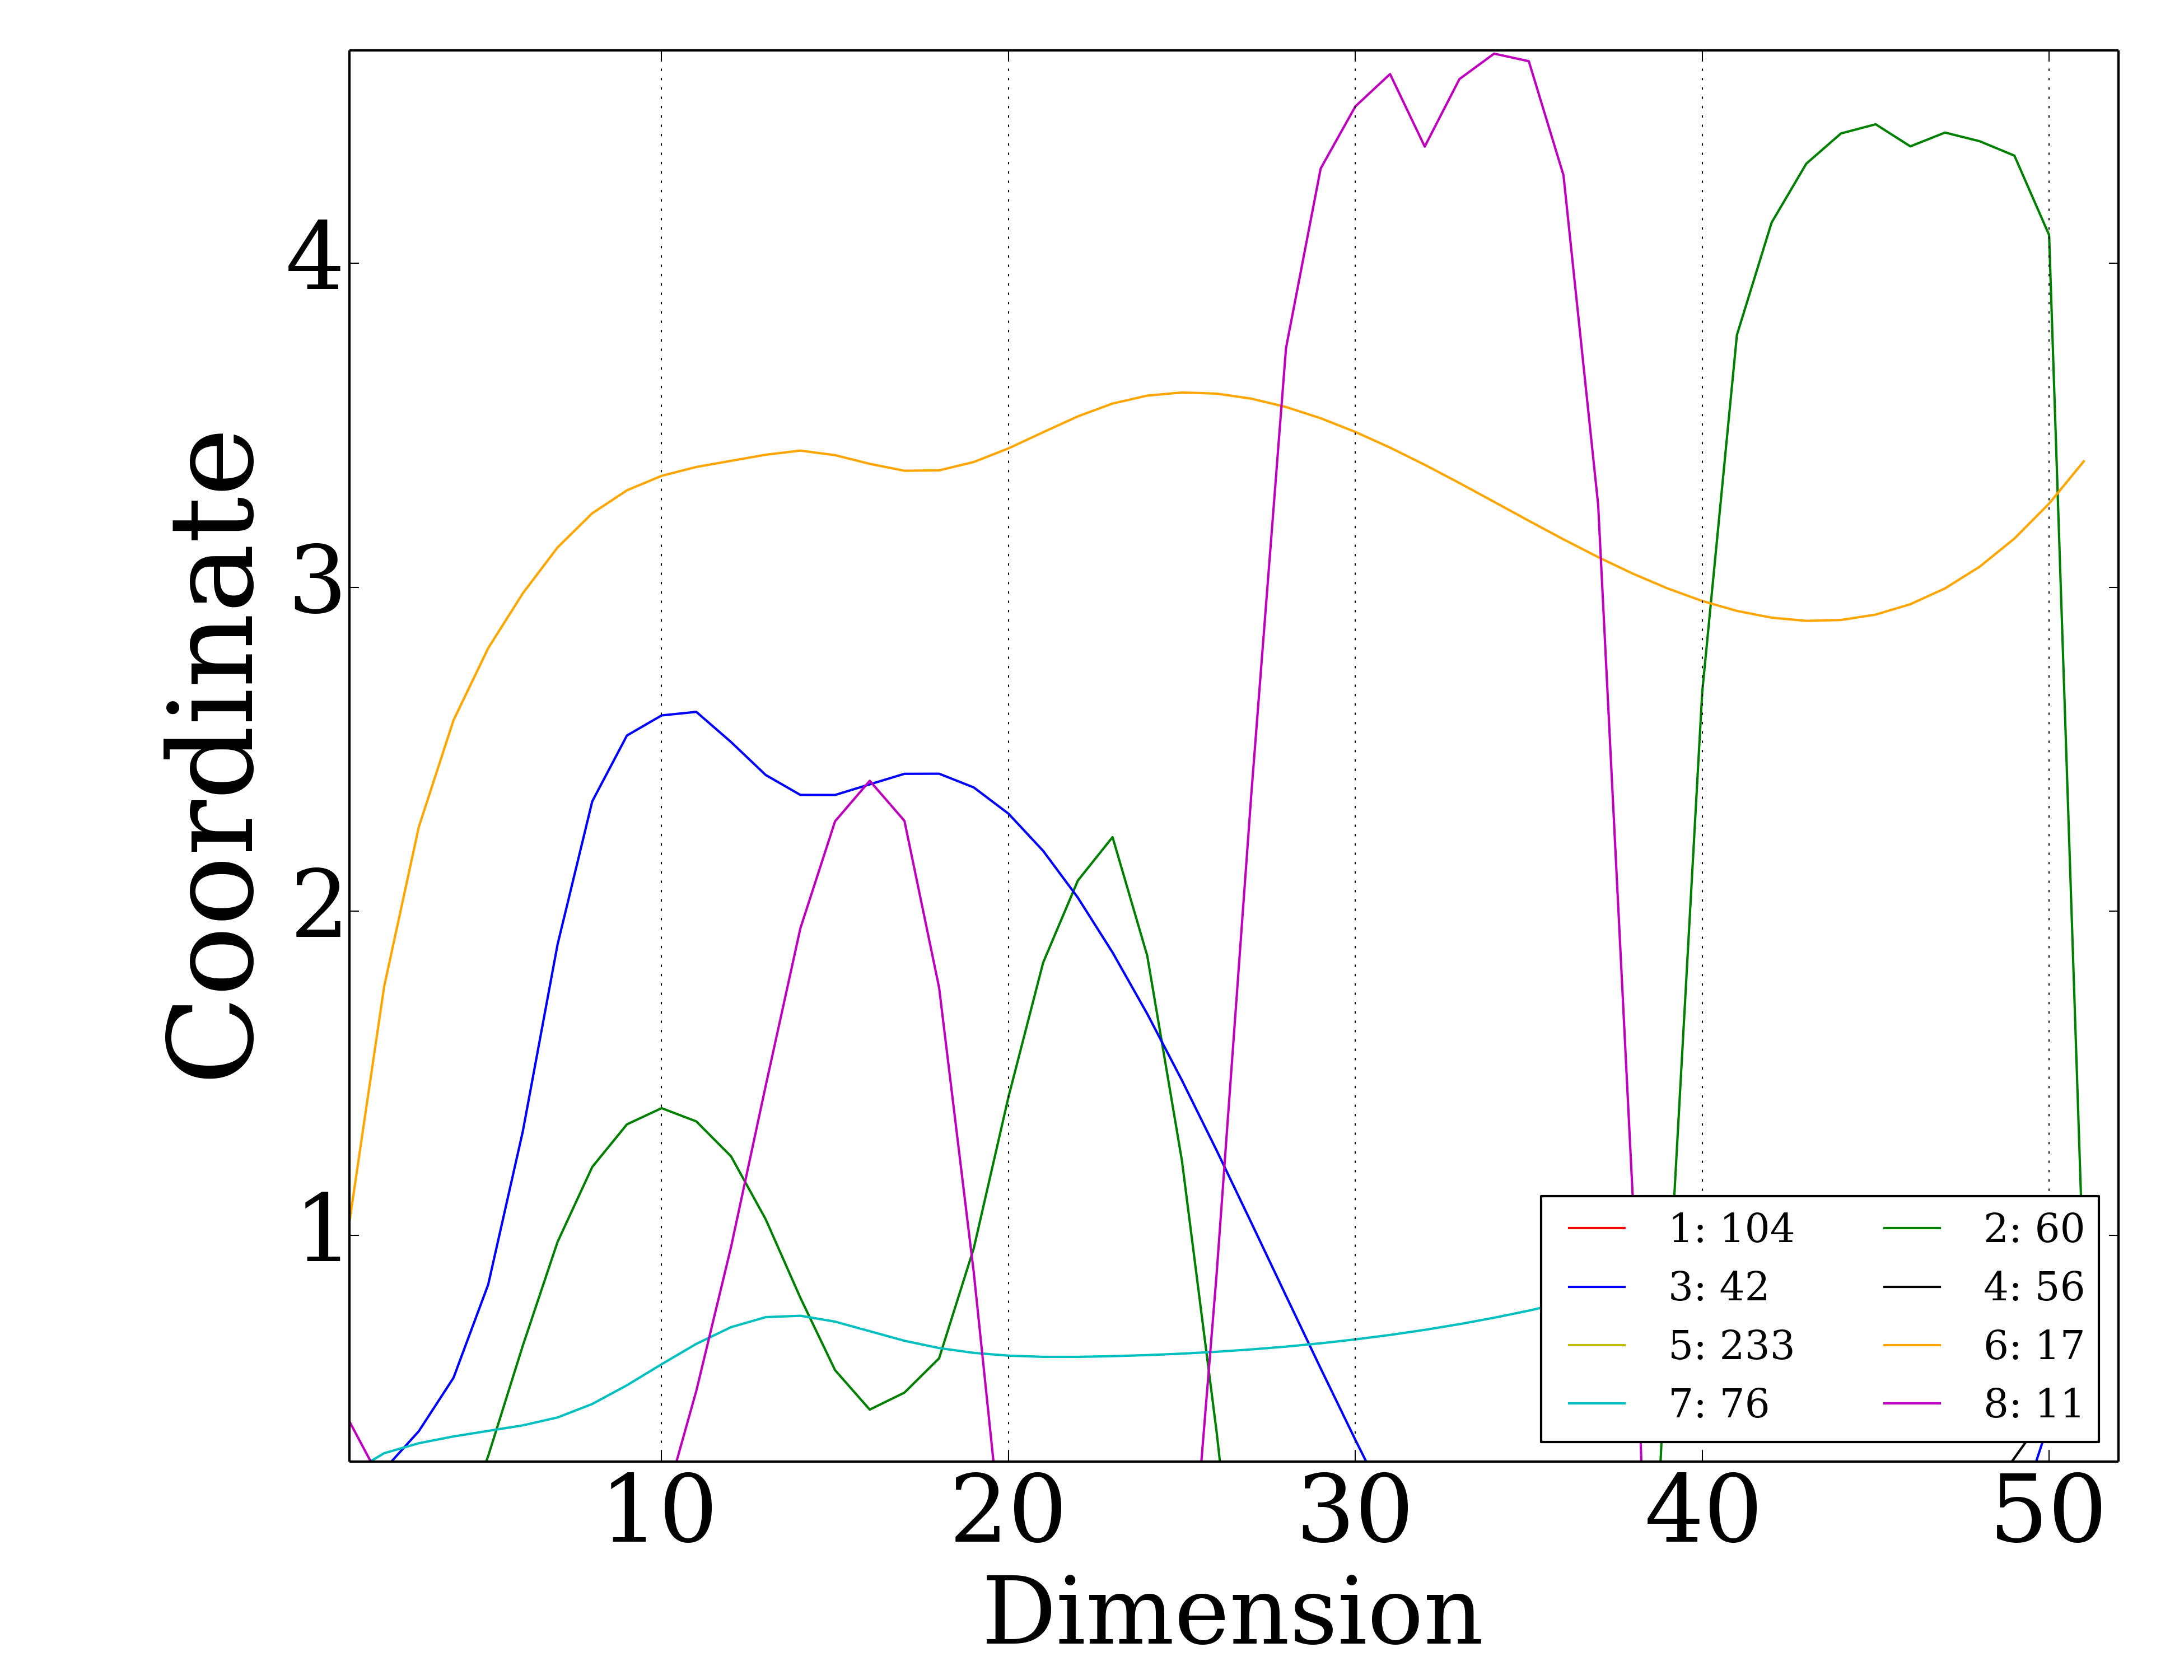
\includegraphics[scale=0.2]{{plots/newdata/centplotlimit}.png}}
\hfill
\subfloat[Centroids]{\includegraphics[scale=0.2]{{plots/newdata/centplot}.png}}
\end{minipage}
\caption{Cluster analysis of mRNA data}
\label{fig:supclust}
\end{figure}
\clearpage

\begin{figure}[ht]
\centering
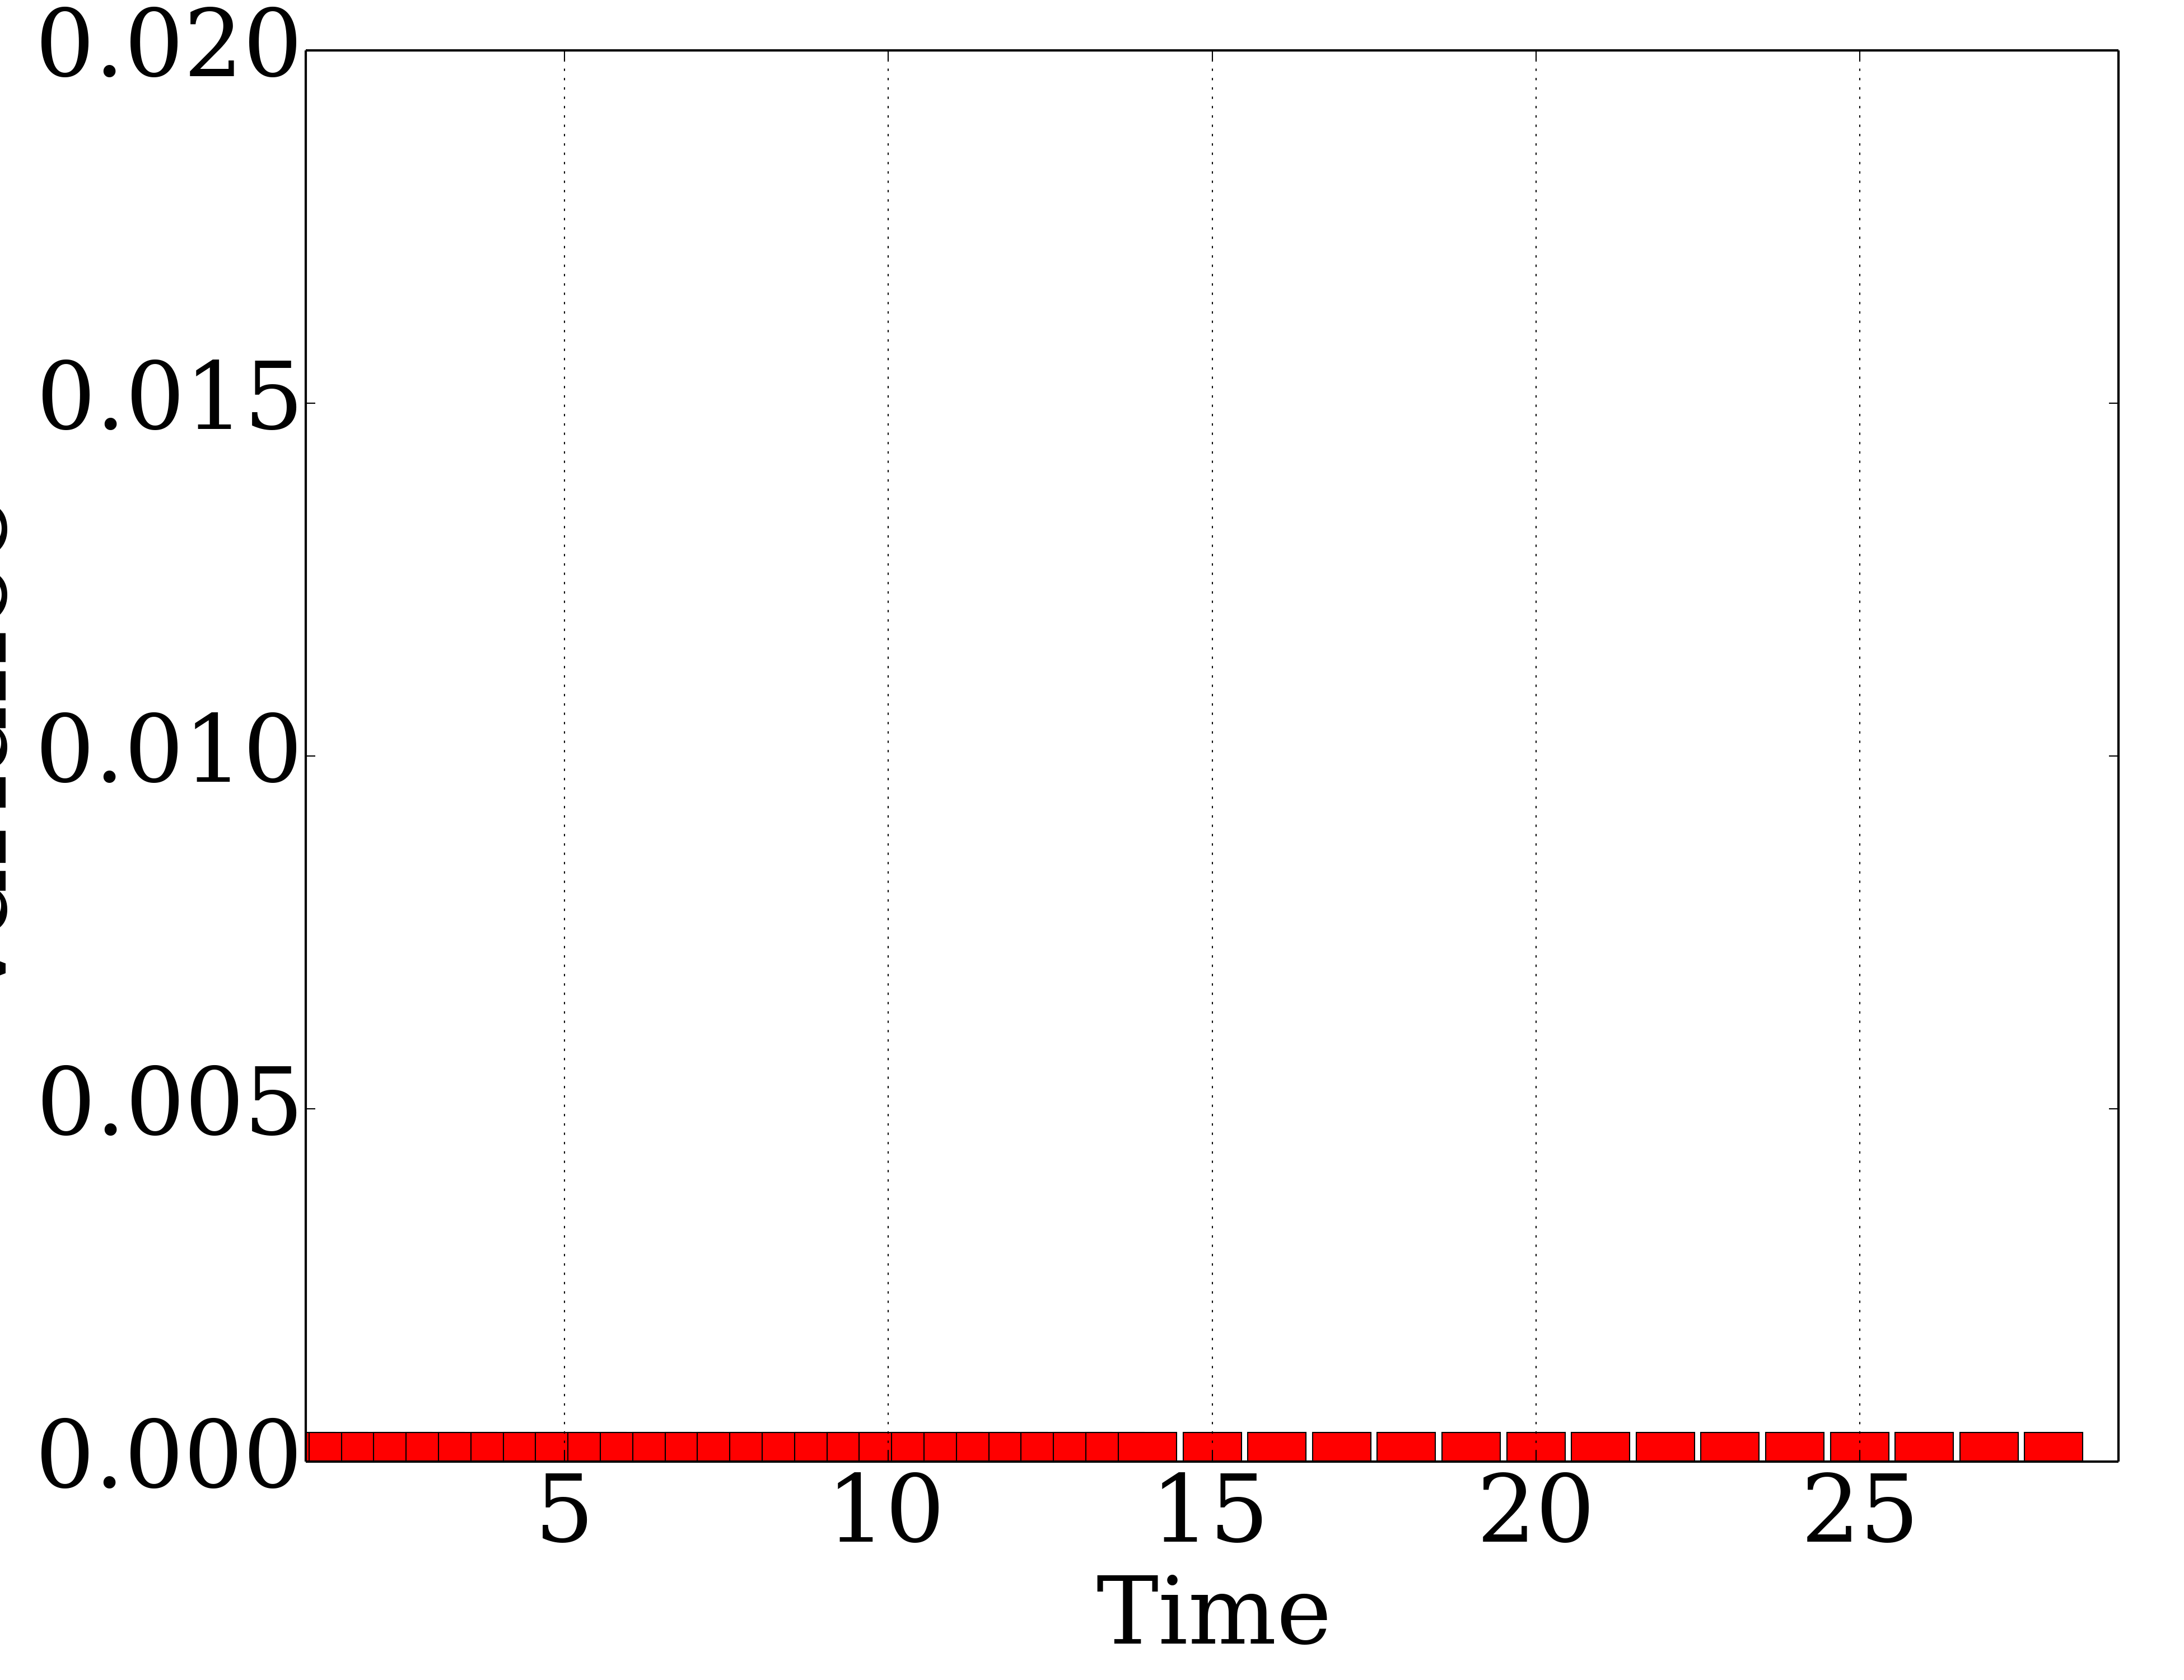
\includegraphics[scale=0.25]{{plots/newdata/timeerror}.png}
\caption{Average noise in each time point}
\label{fig:sup1}
\end{figure}
\clearpage

\begin{figure}
\centering
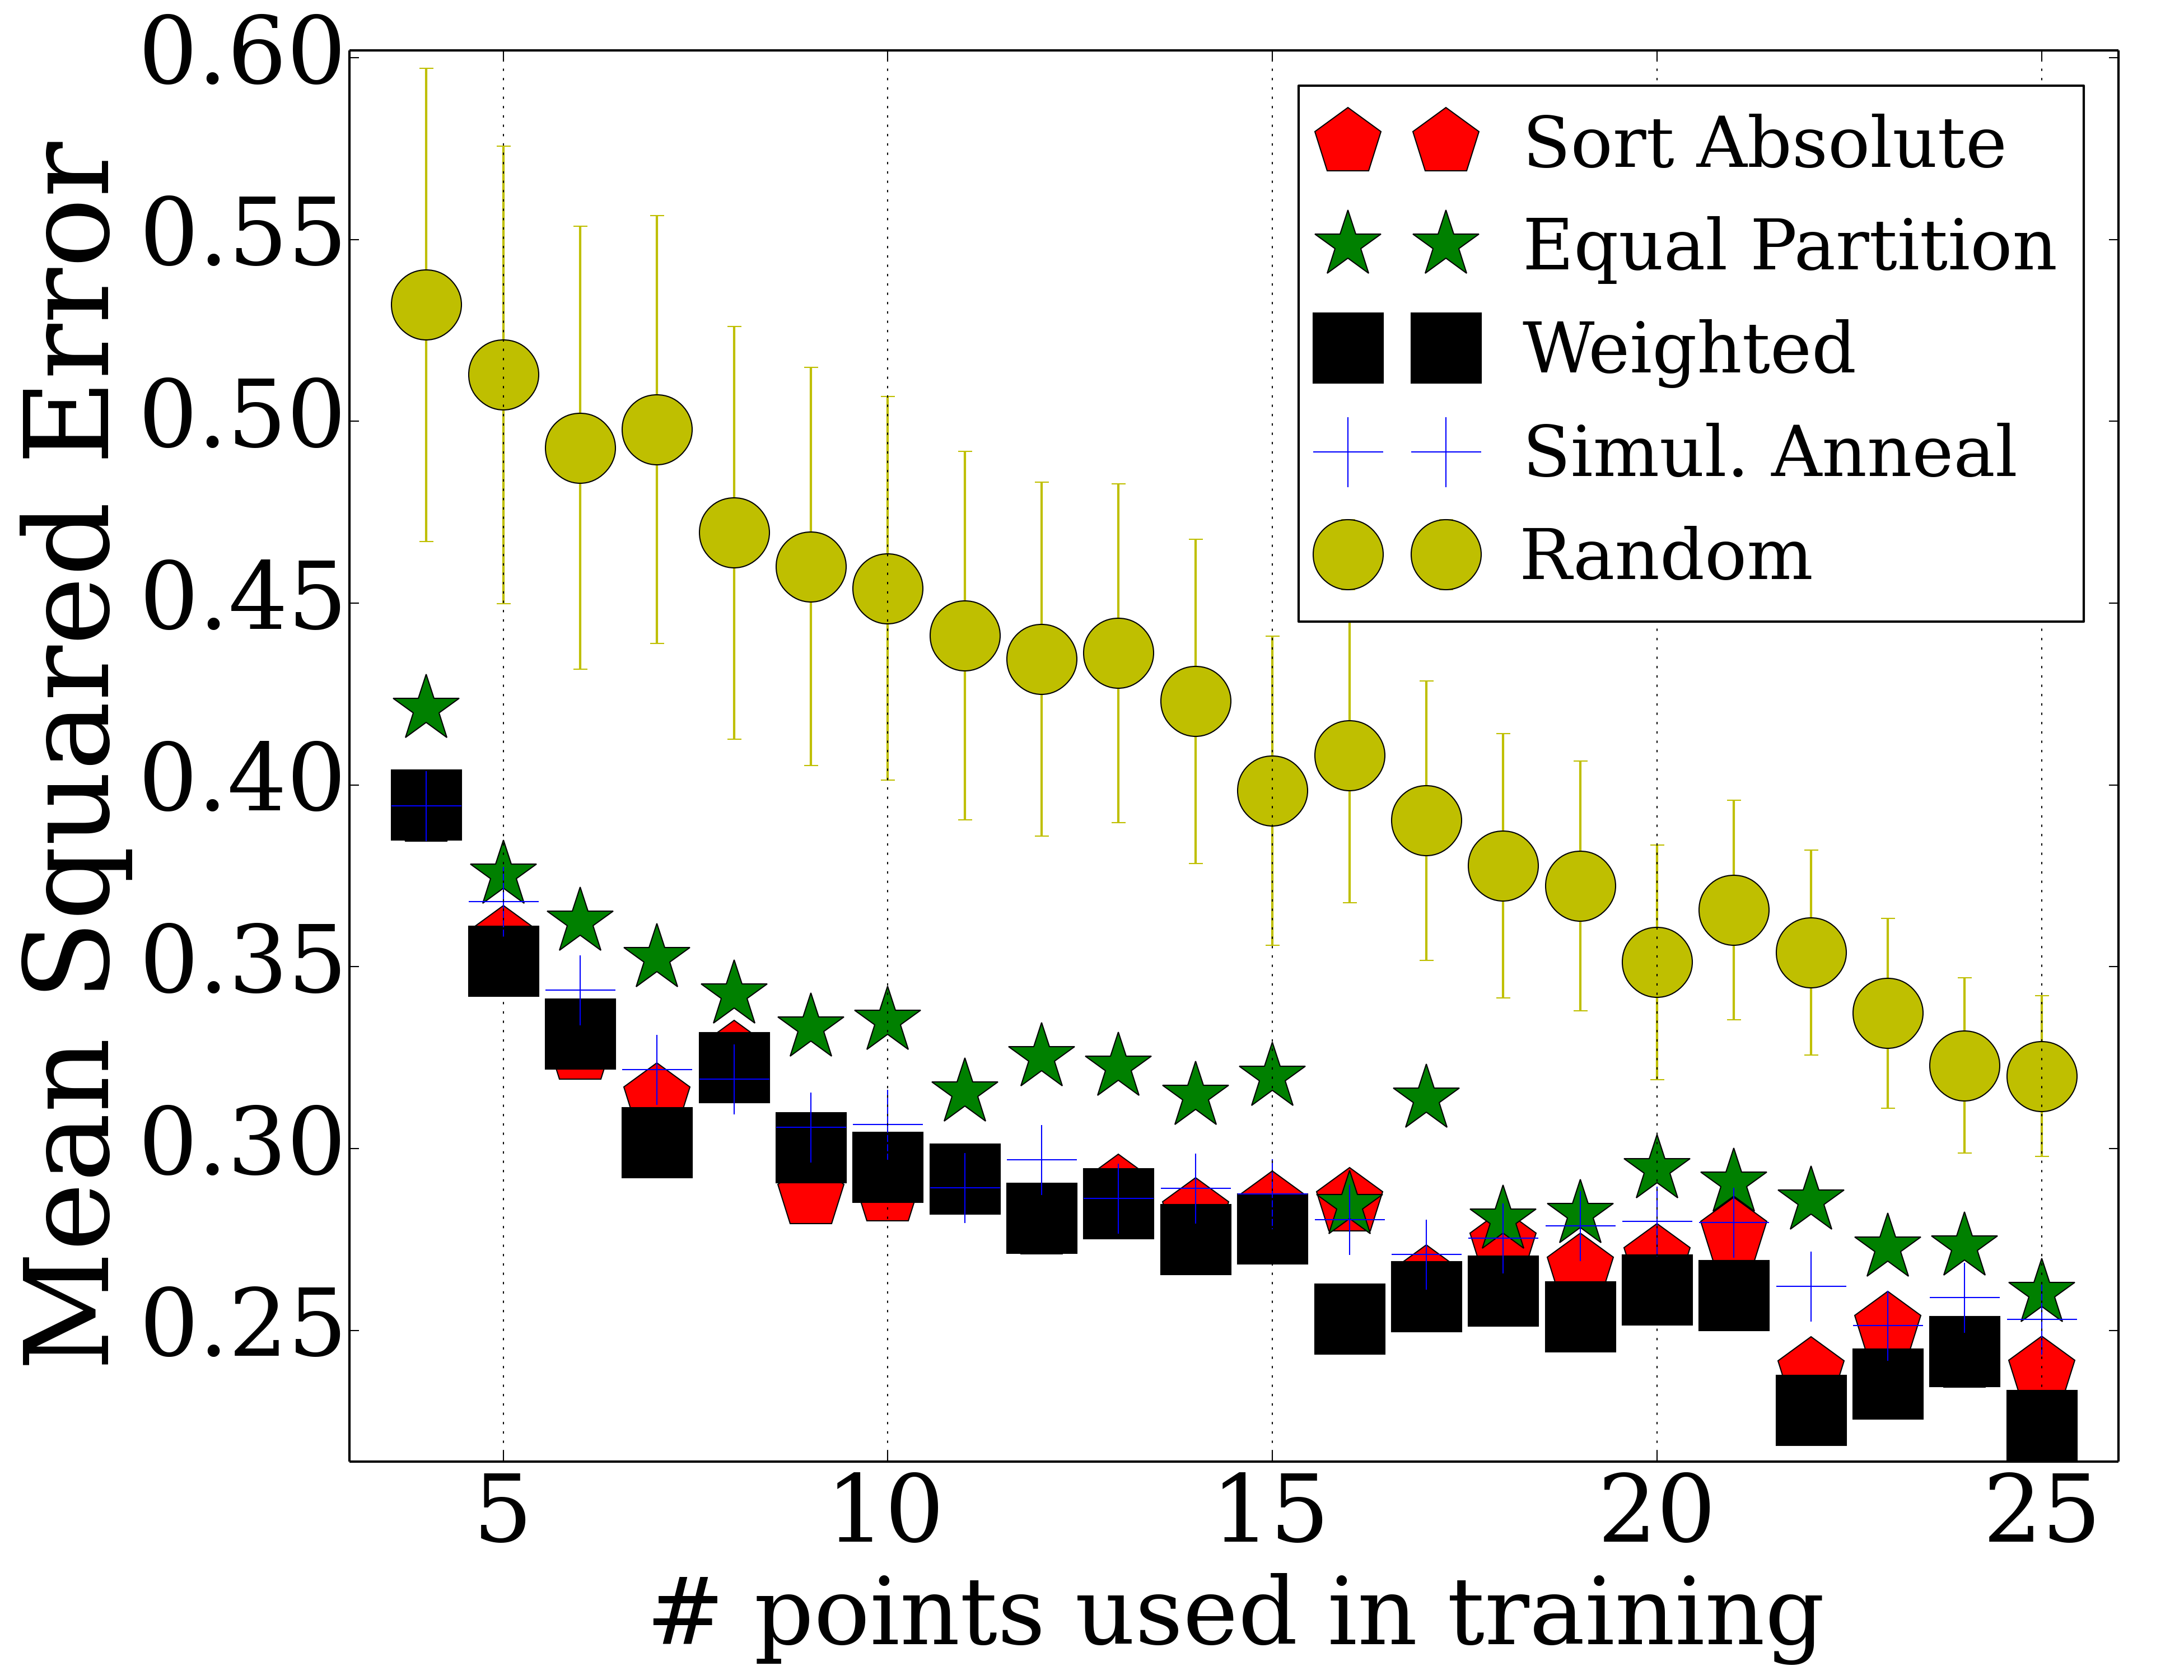
\includegraphics[scale=0.25]{{plots/newdata/performRL2}.png}
\caption{Performance of \TPS by increasing number of selected points}
\label{fig:sup2}
\end{figure}
\clearpage

\begin{figure}
\centering
\begin{minipage}{1.0\textwidth}
\subfloat[ERB]{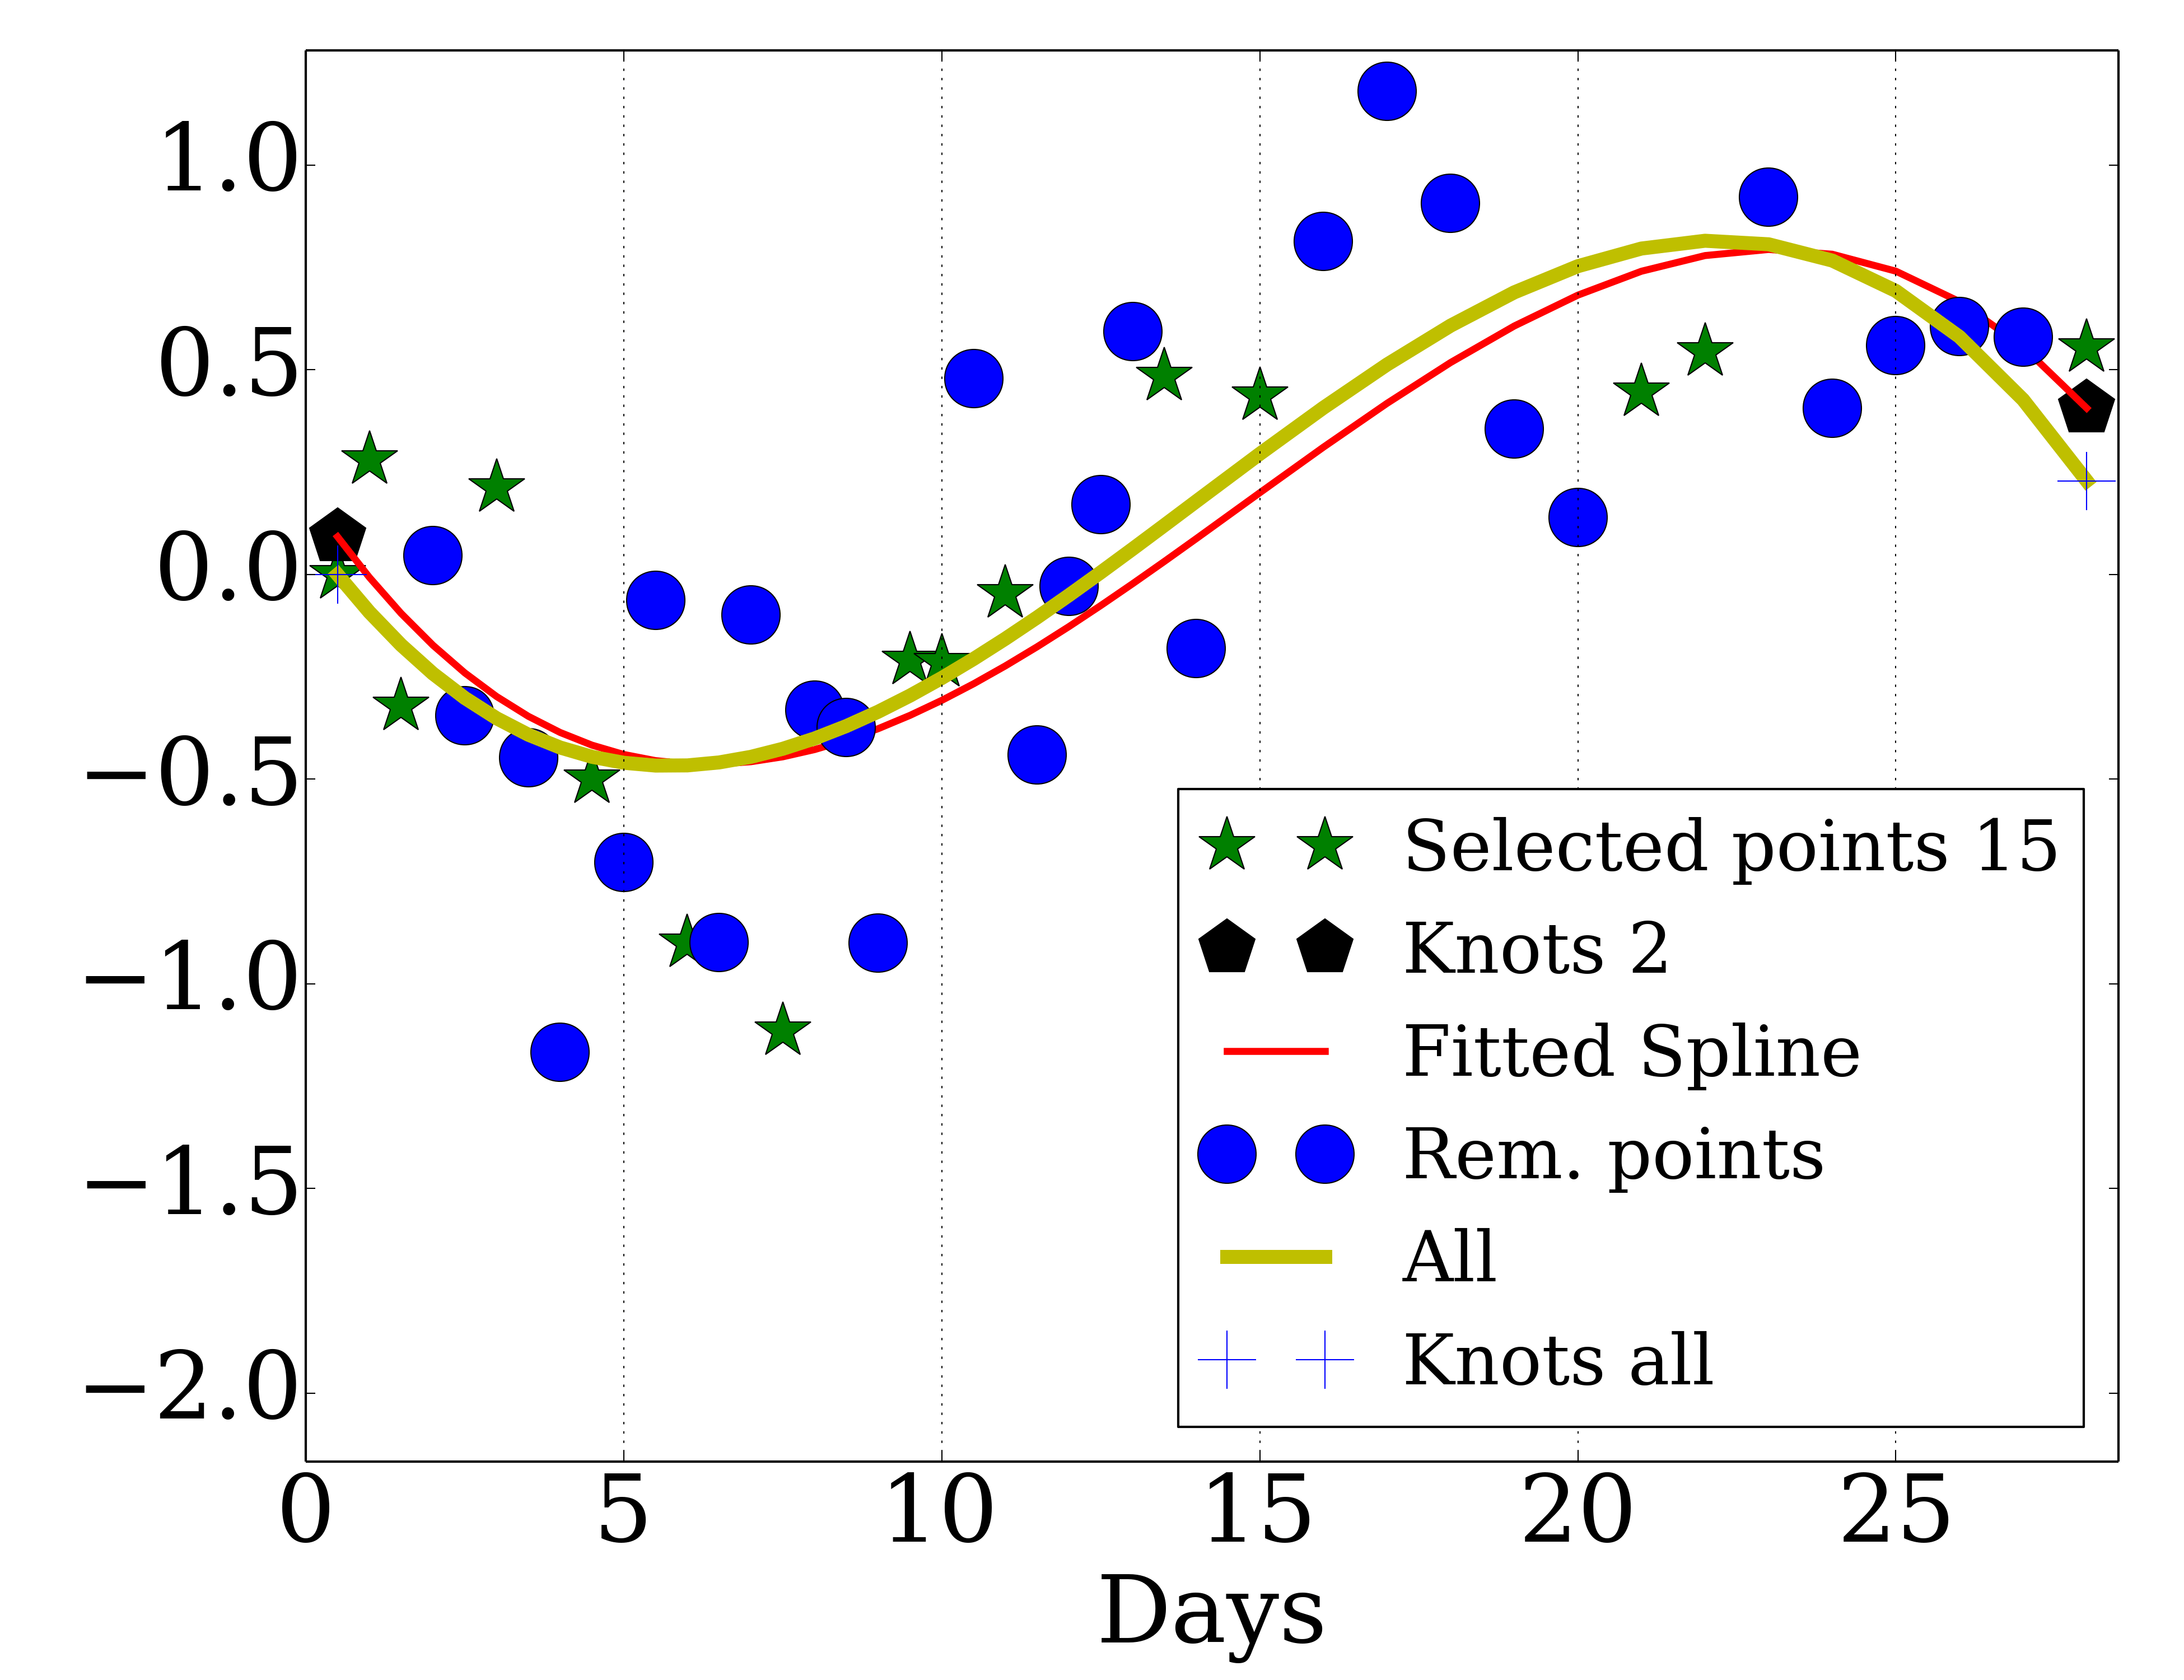
\includegraphics[scale=0.12]{{plots/newdata/splineplots15/ERB_15_all}.png}}
\hfill
\subfloat[NME3]{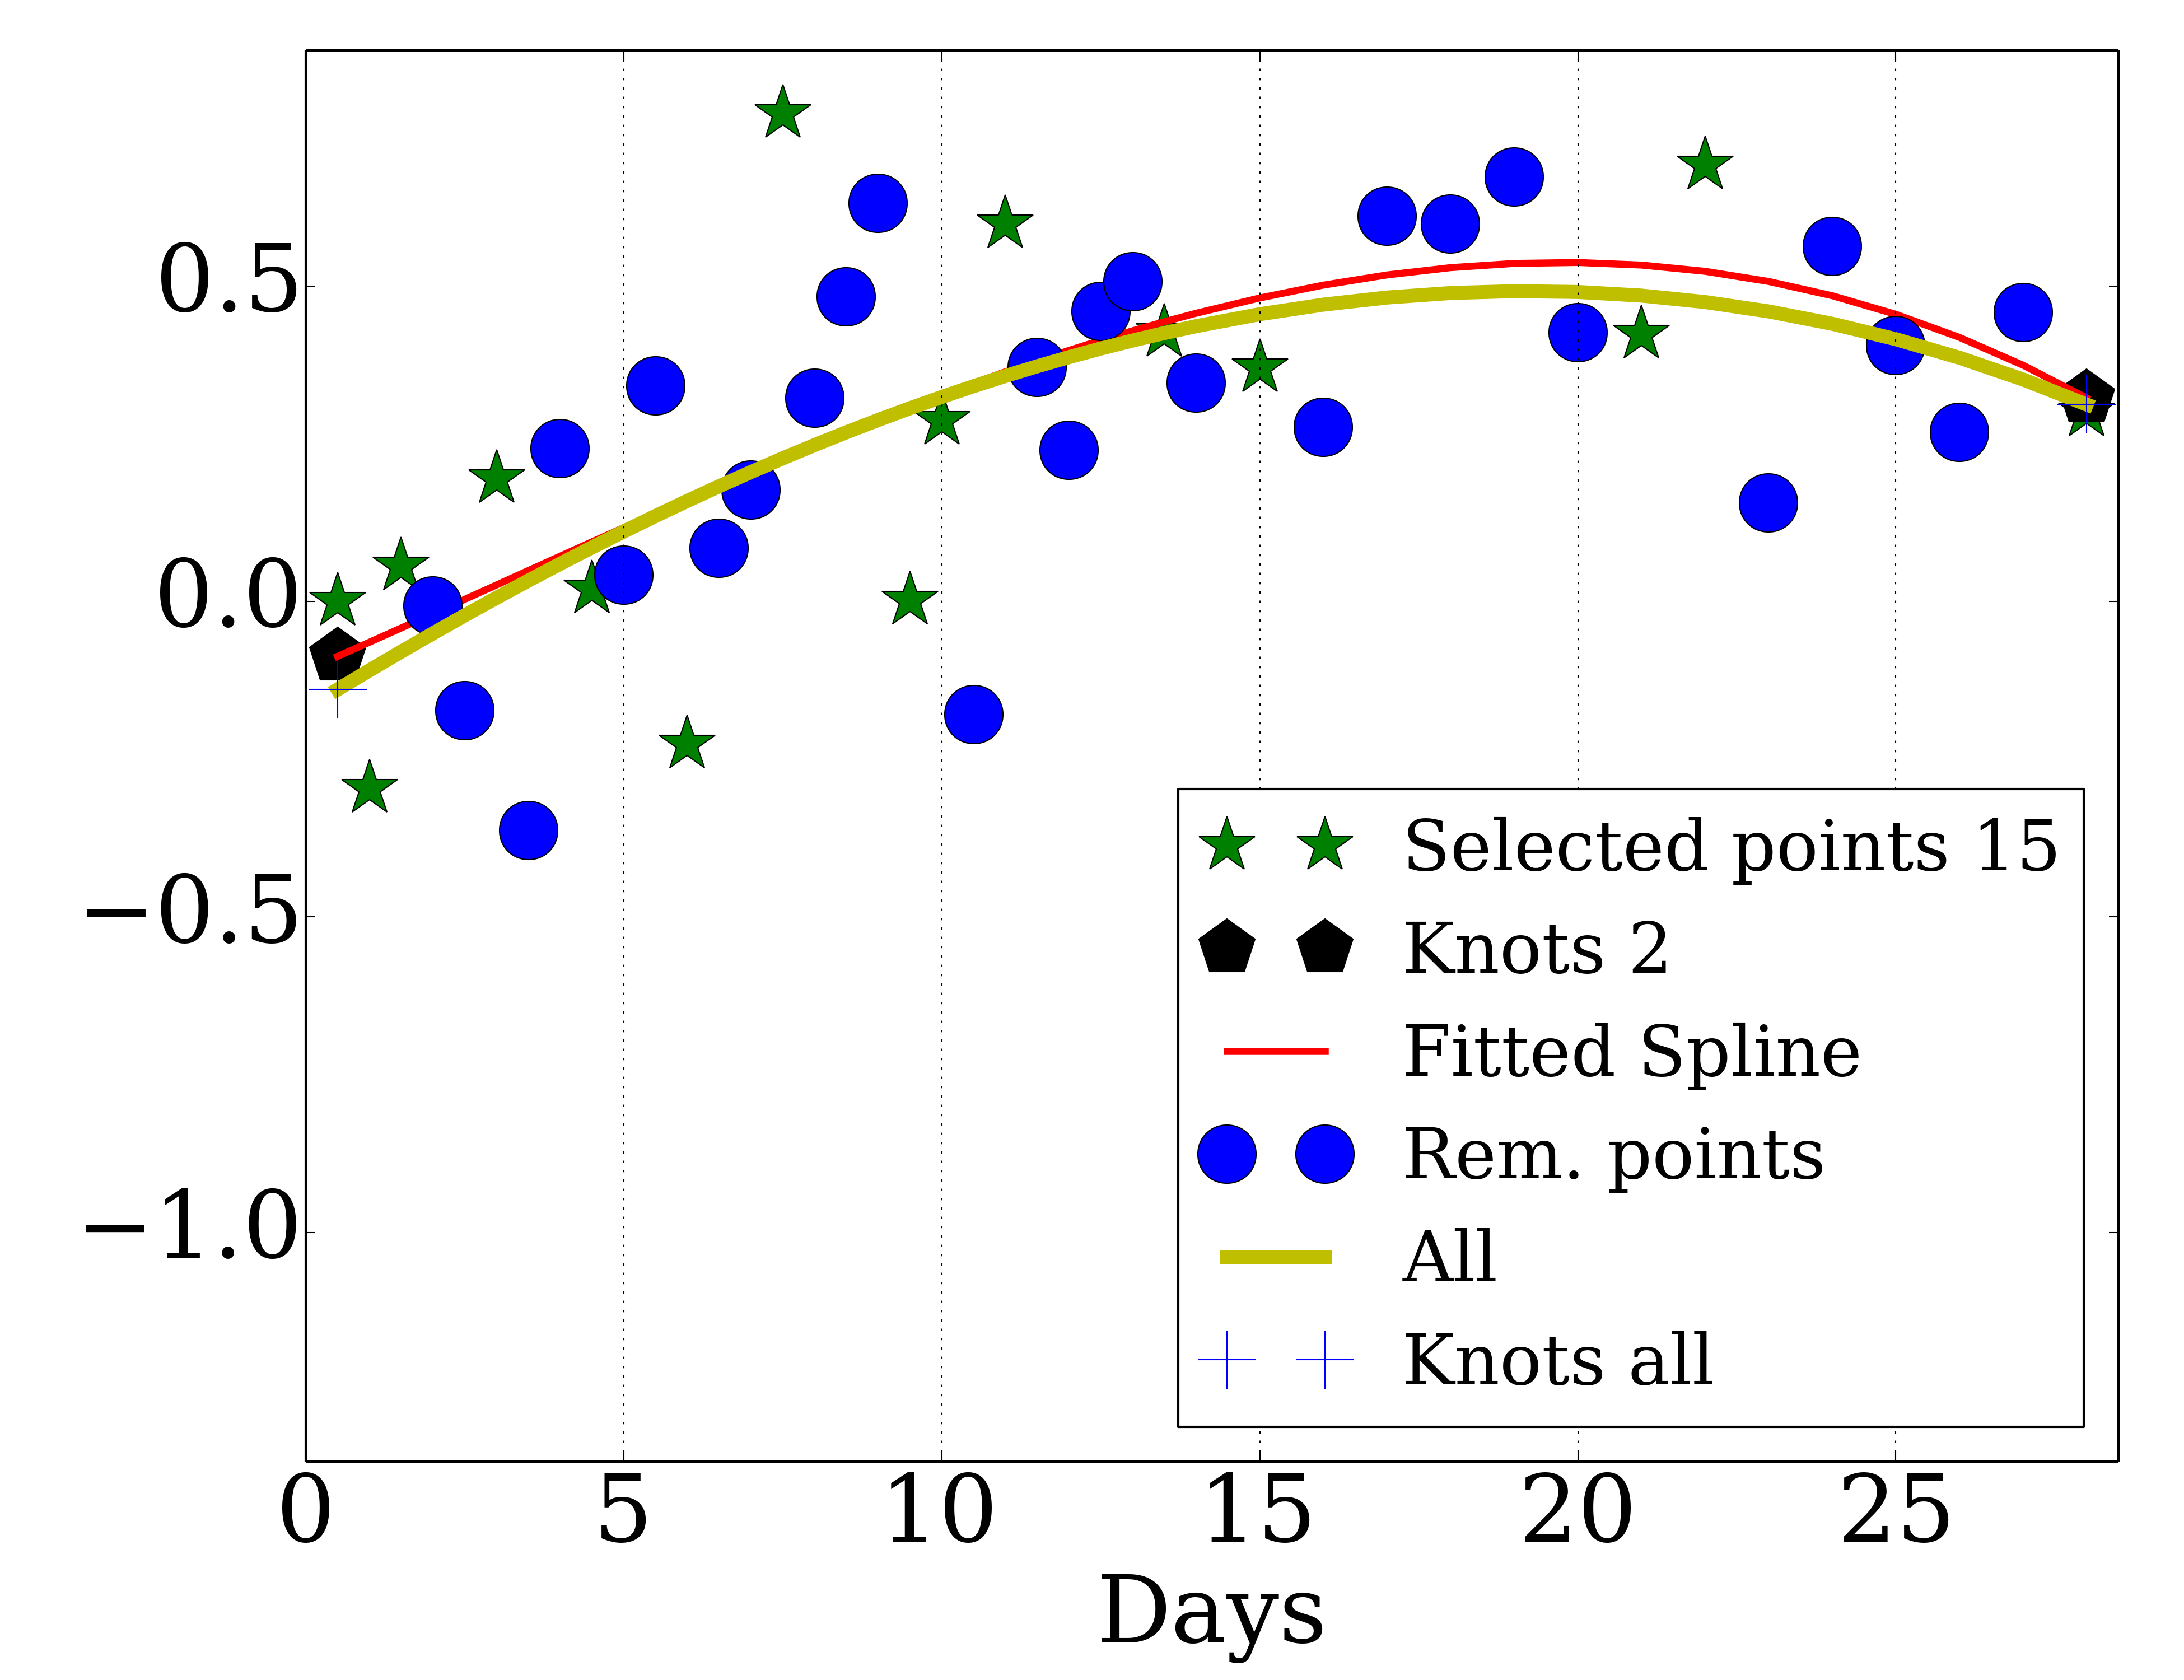
\includegraphics[scale=0.12]{{plots/newdata/splineplots15/NME3_15_all}.png}}
\hfill
\subfloat[POL2RA]{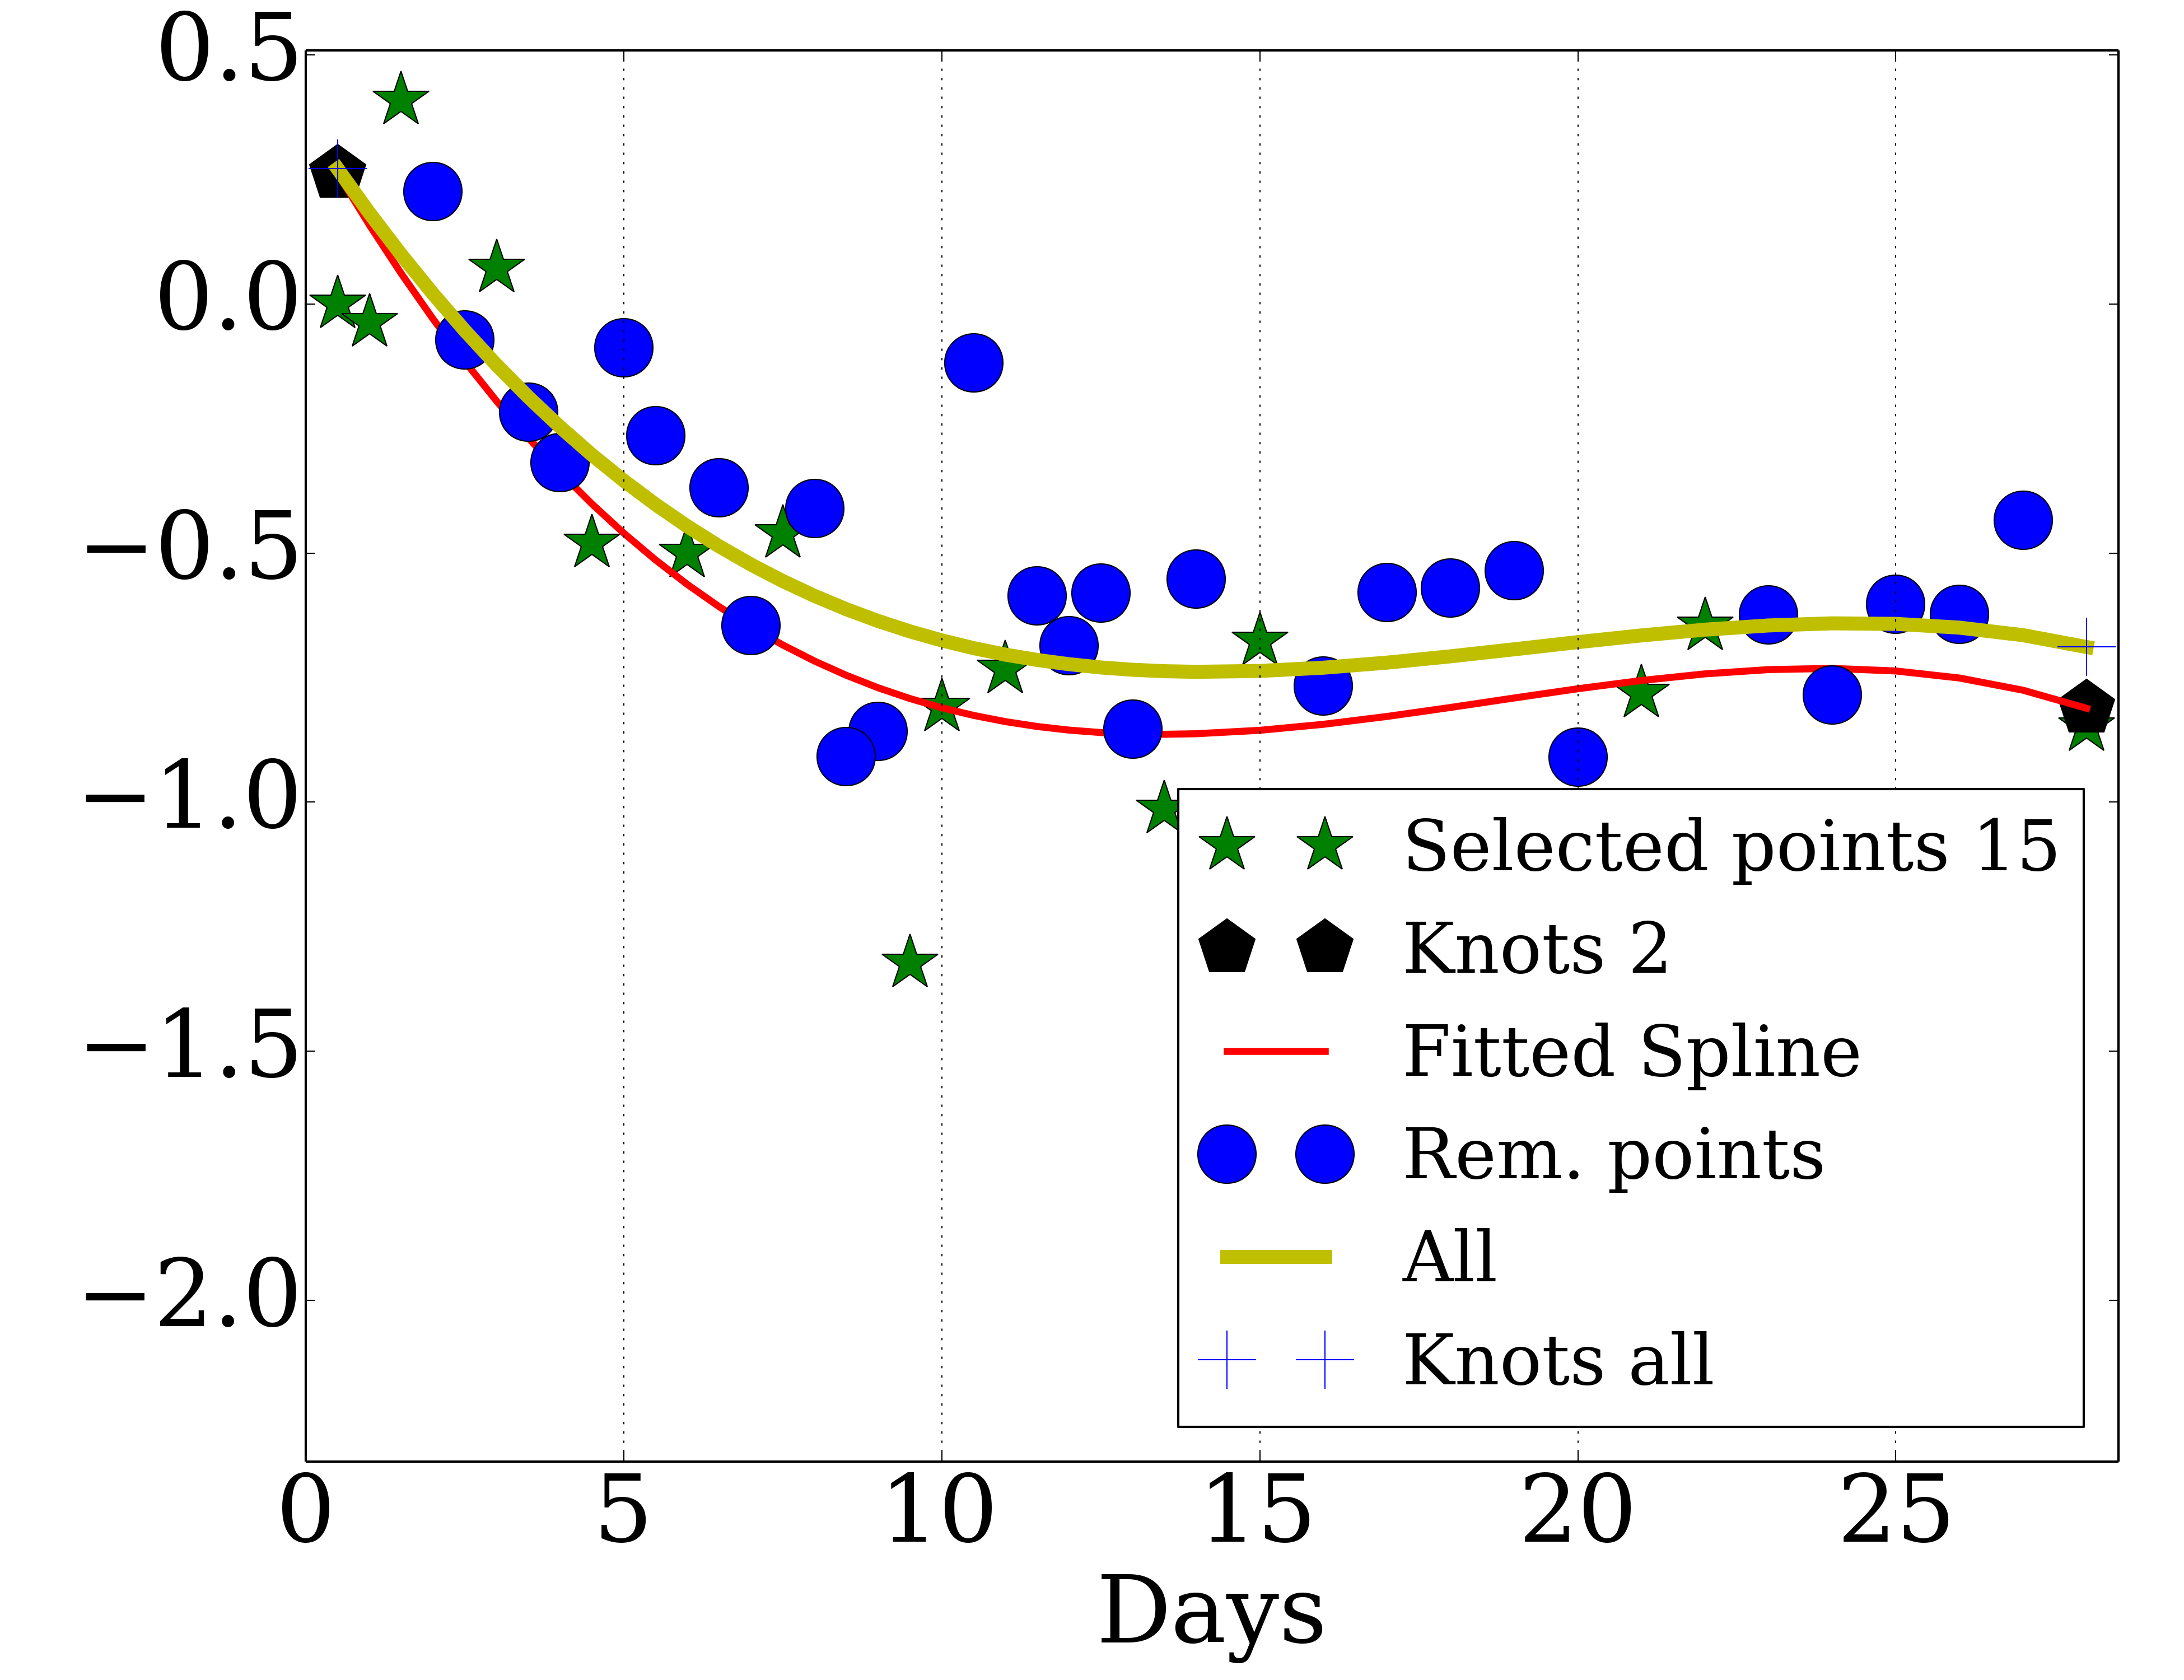
\includegraphics[scale=0.12]{{plots/newdata/splineplots15/polr2a_15_all}.png}}
\hfill
\end{minipage}
\caption{Expression profiles over several genes a) ERB, b) NME3, c) POL2RA}
\label{fig:sup3}
\end{figure}
\clearpage

\begin{figure}
\centering
\begin{minipage}{1.0\textwidth}
\subfloat[PDGFRA]{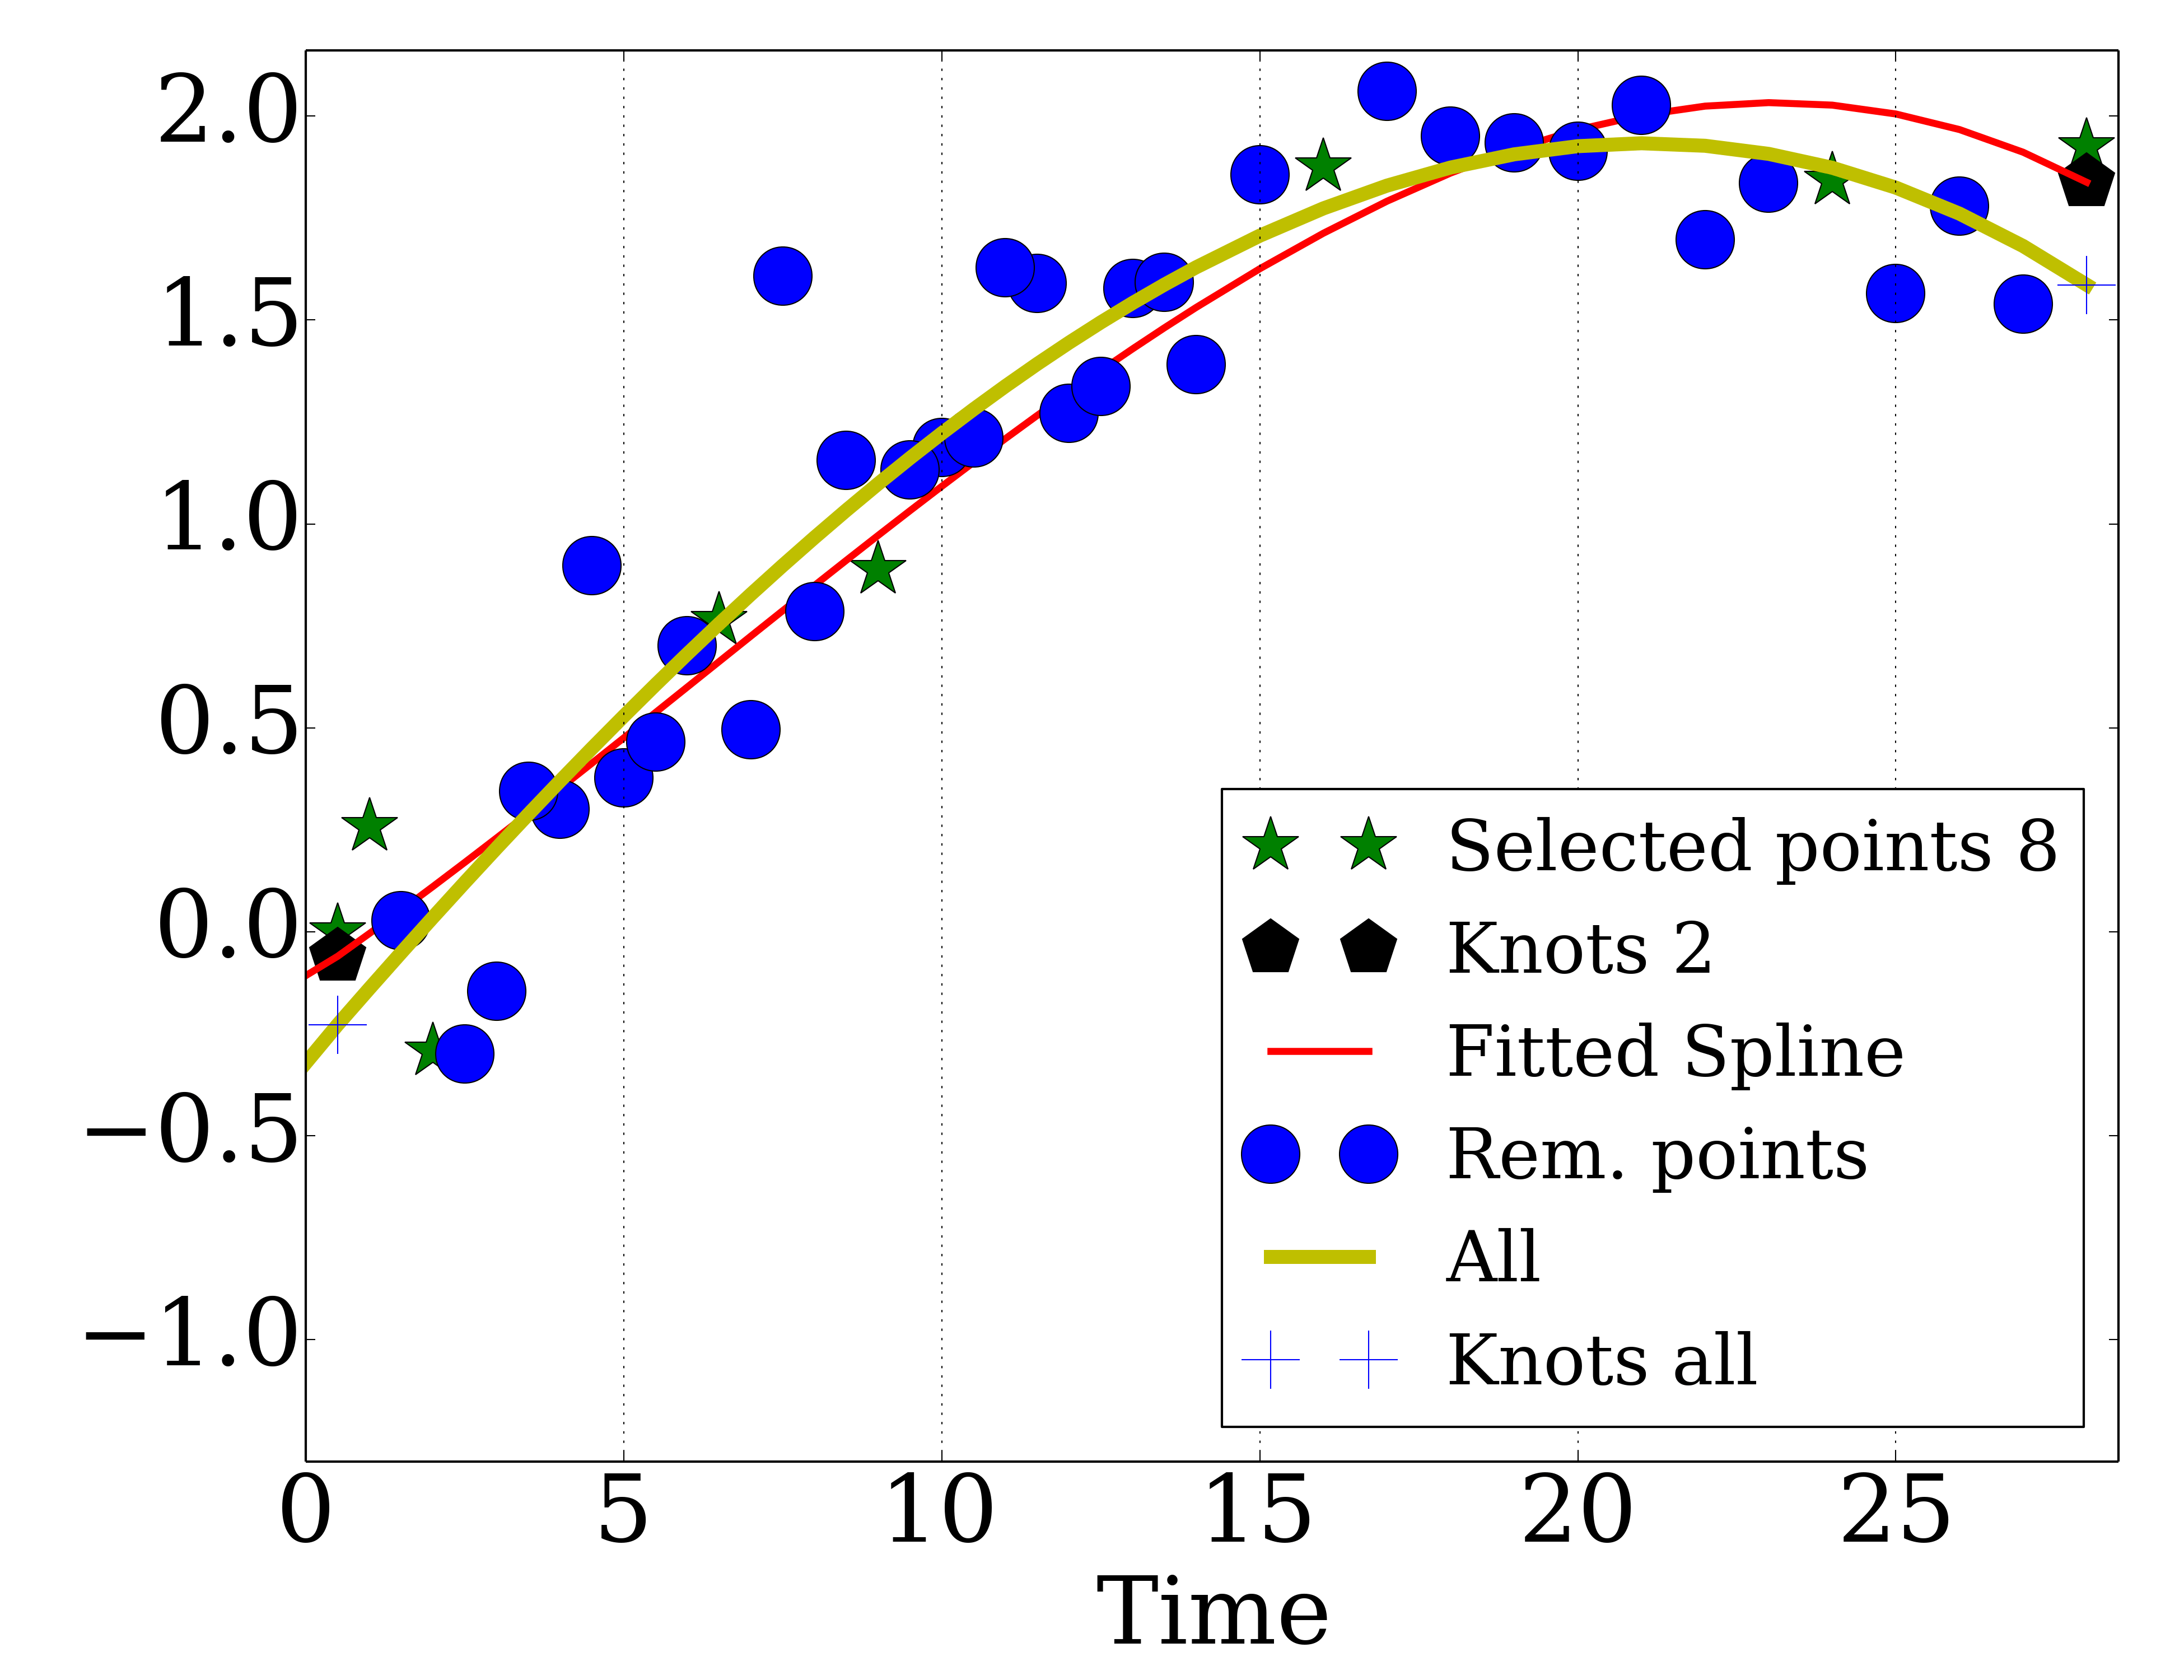
\includegraphics[scale=0.12]{{plots/newdata/splineplots8/PDGFRA_8_all}.png}}
\hfill
\subfloat[ELN]{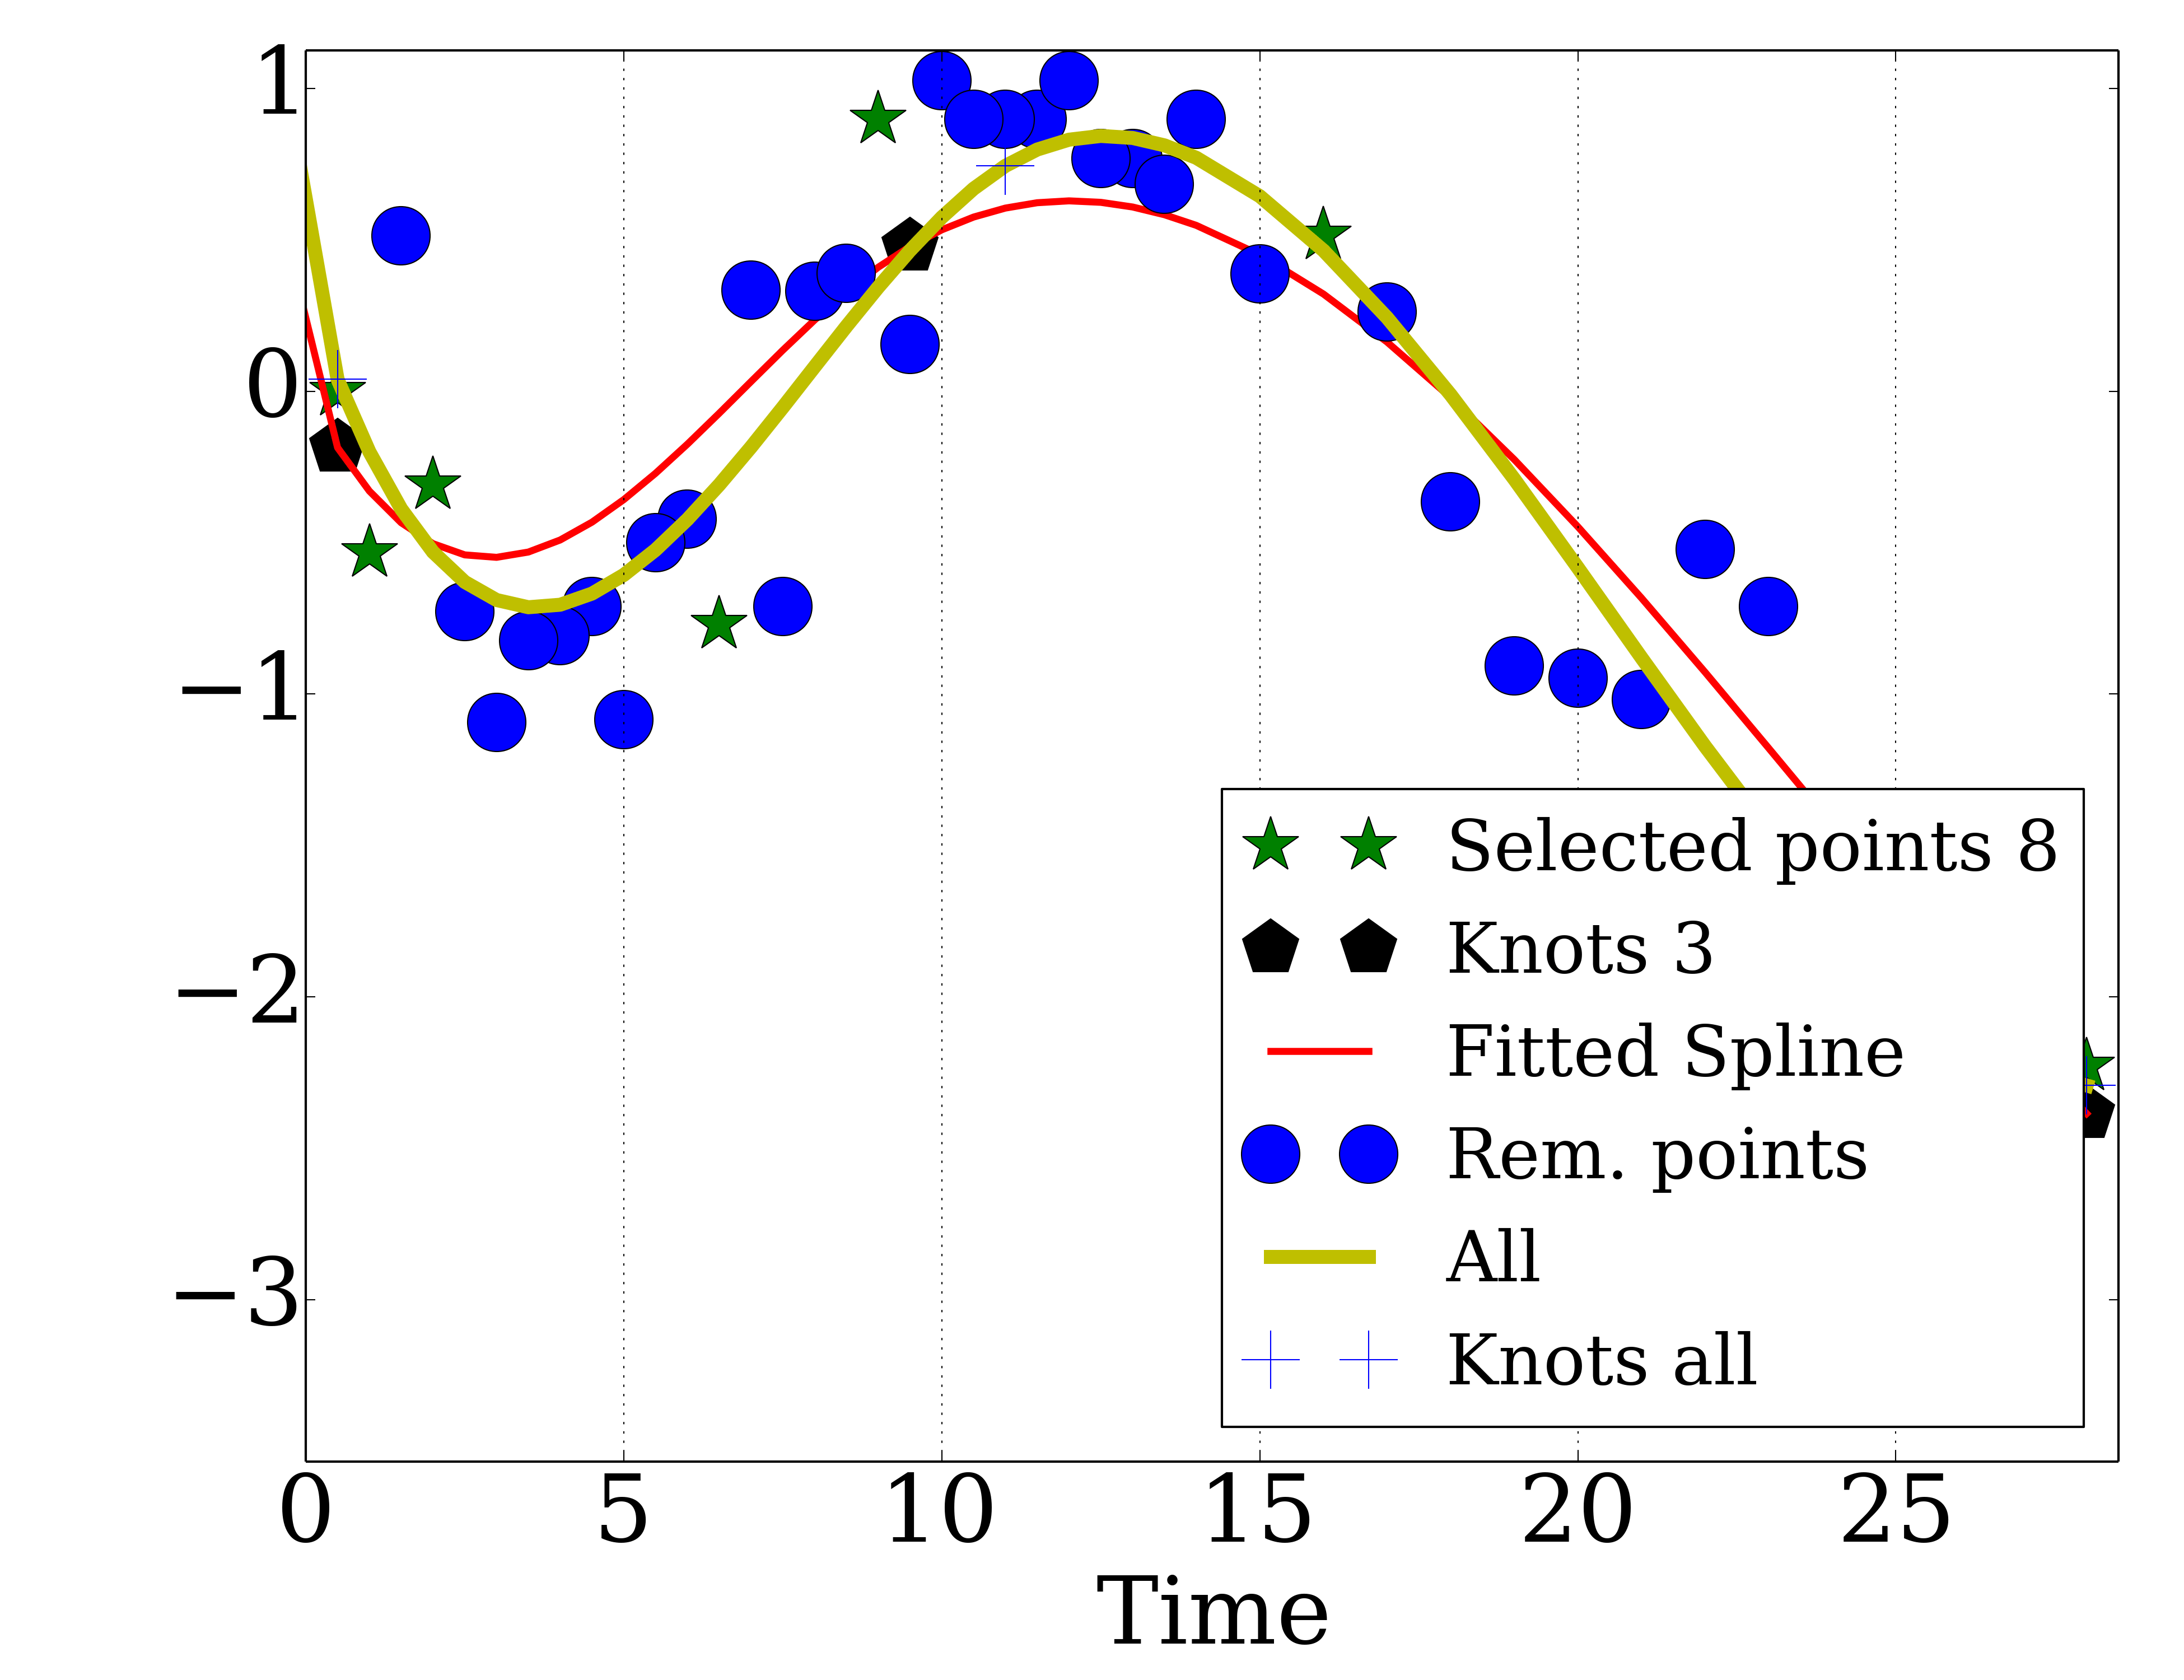
\includegraphics[scale=0.12]{{plots/newdata/splineplots8/Eln_8_all}.png}}
\hfill
\subfloat[INMT]{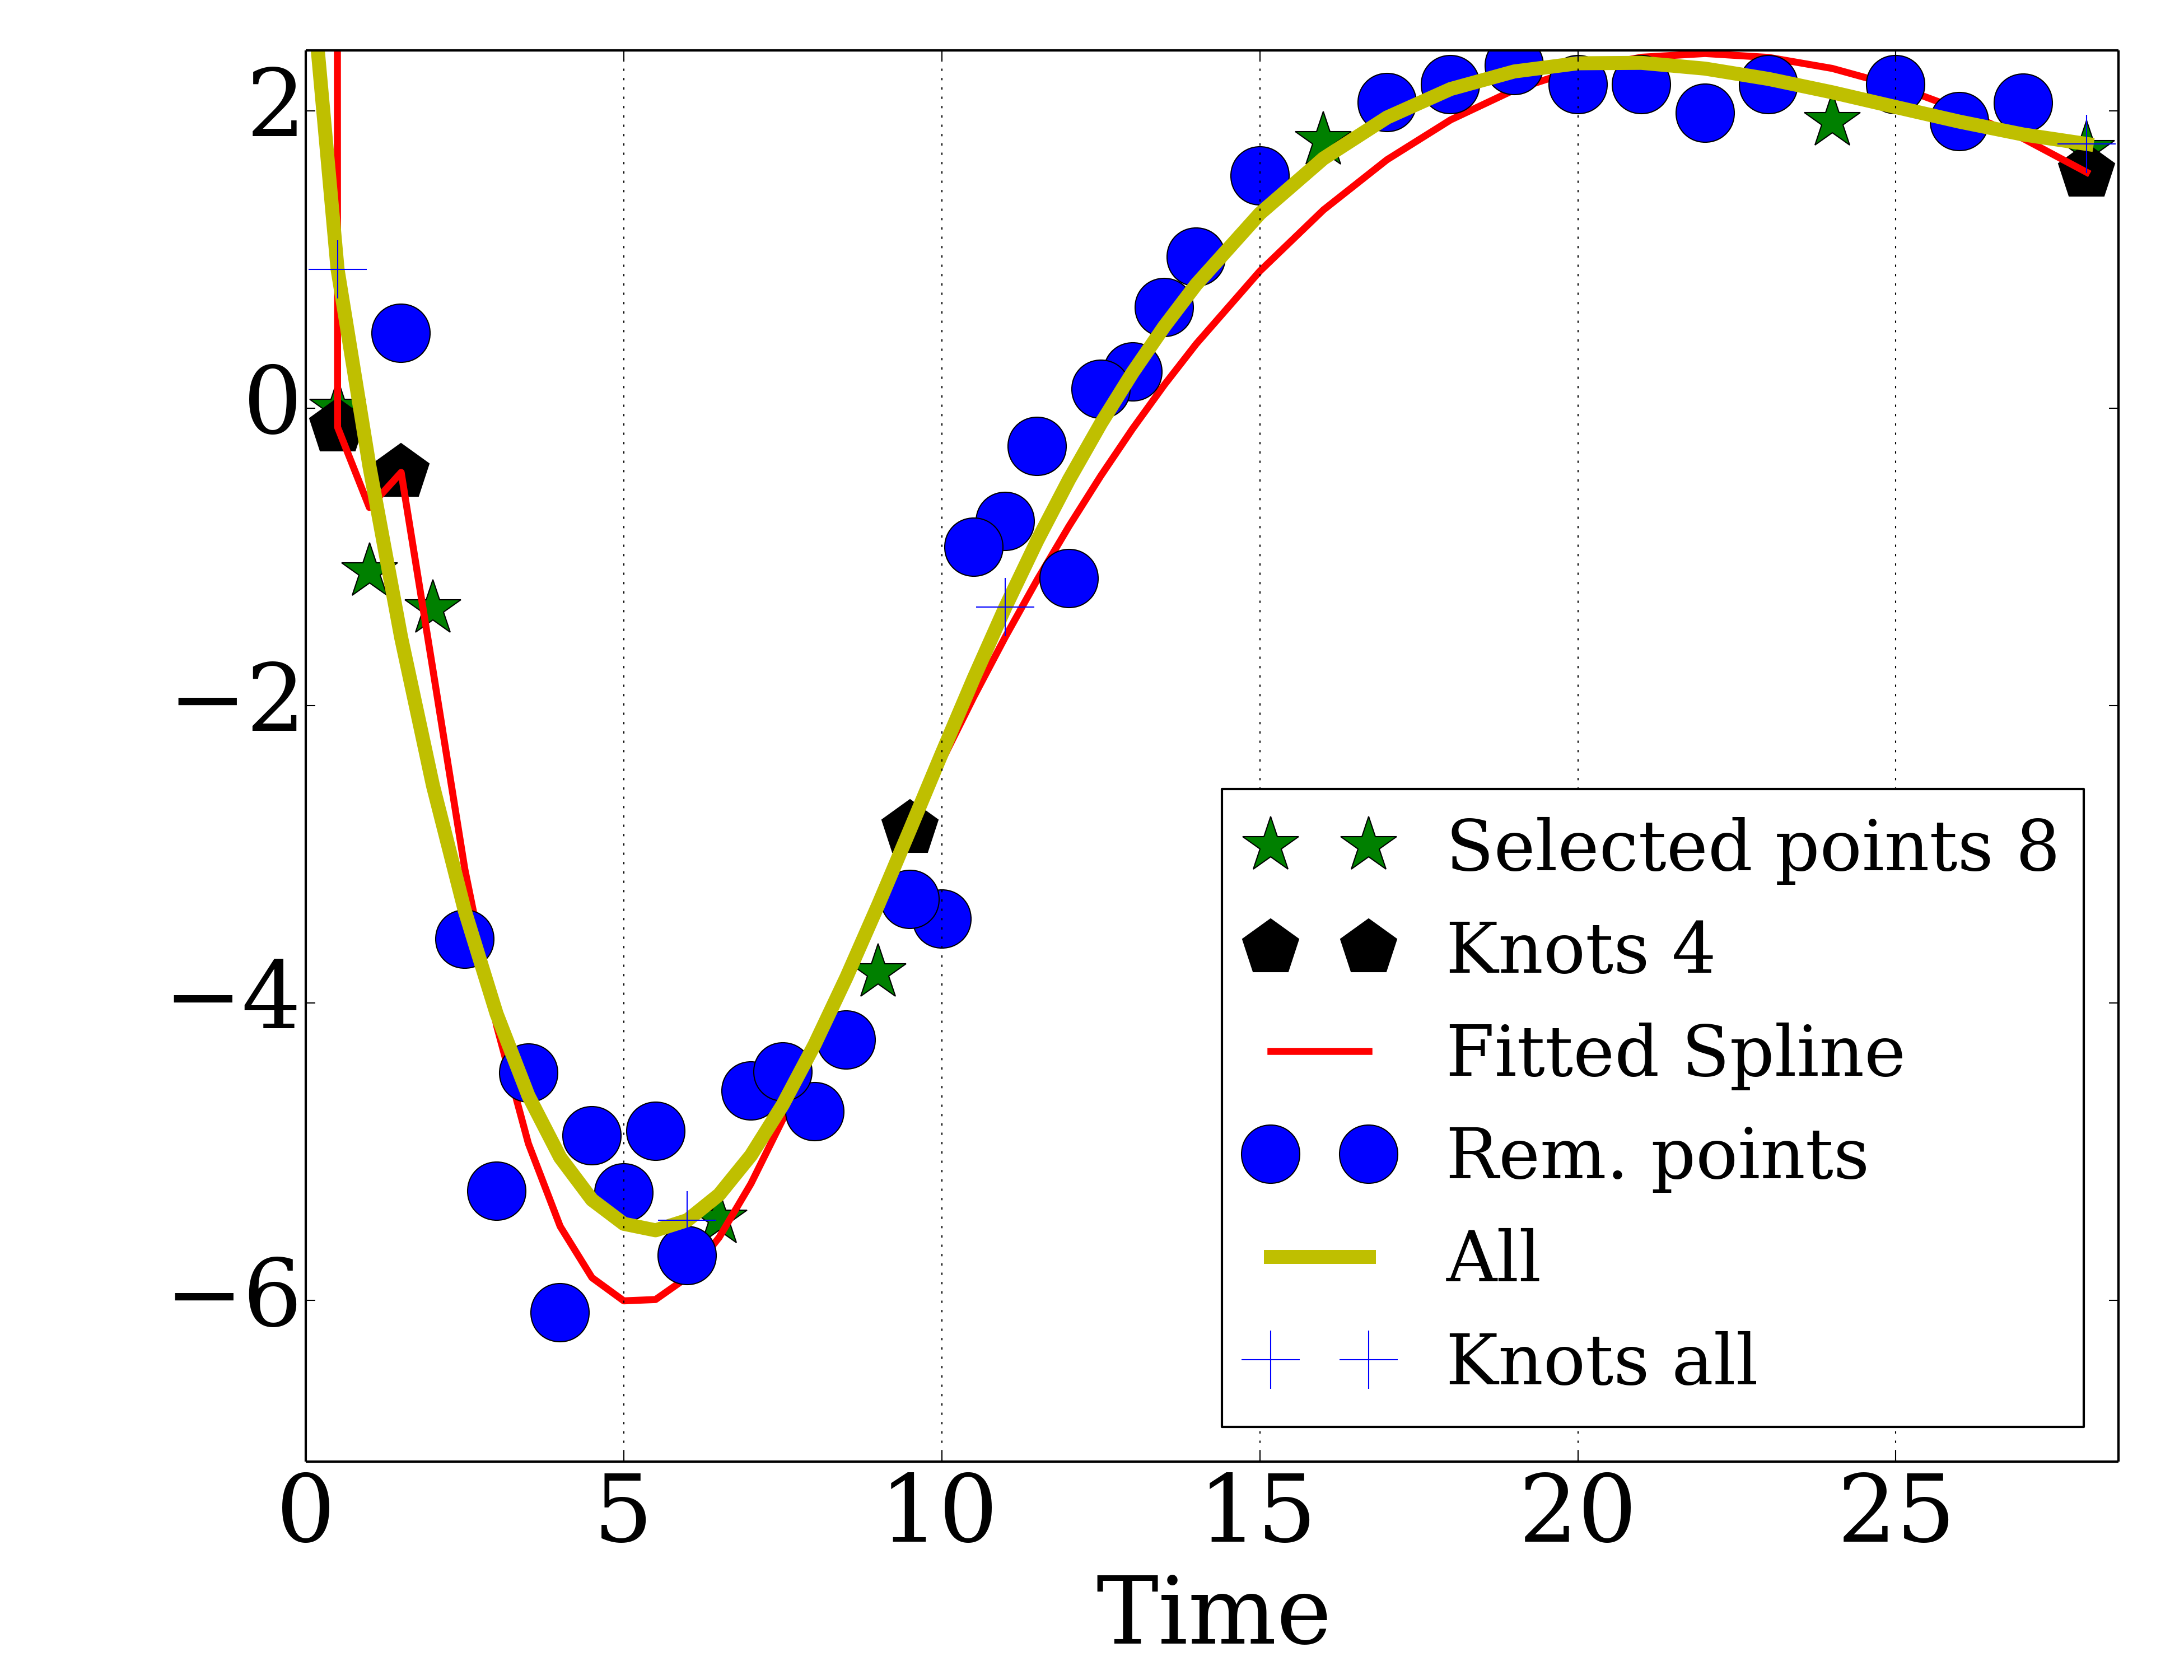
\includegraphics[scale=0.12]{{plots/newdata/splineplots8/INMT_8_all}.png}}
\hfill
\end{minipage}
\caption{Reconstructed expression profiles by $8$ points over genes a) PDGFRA, b) ELN, c) INMT}
\label{fig:sup4}
\end{figure}
\clearpage

\begin{figure}
\begin{minipage}{1.0\textwidth}
\subfloat[PDGFRA]{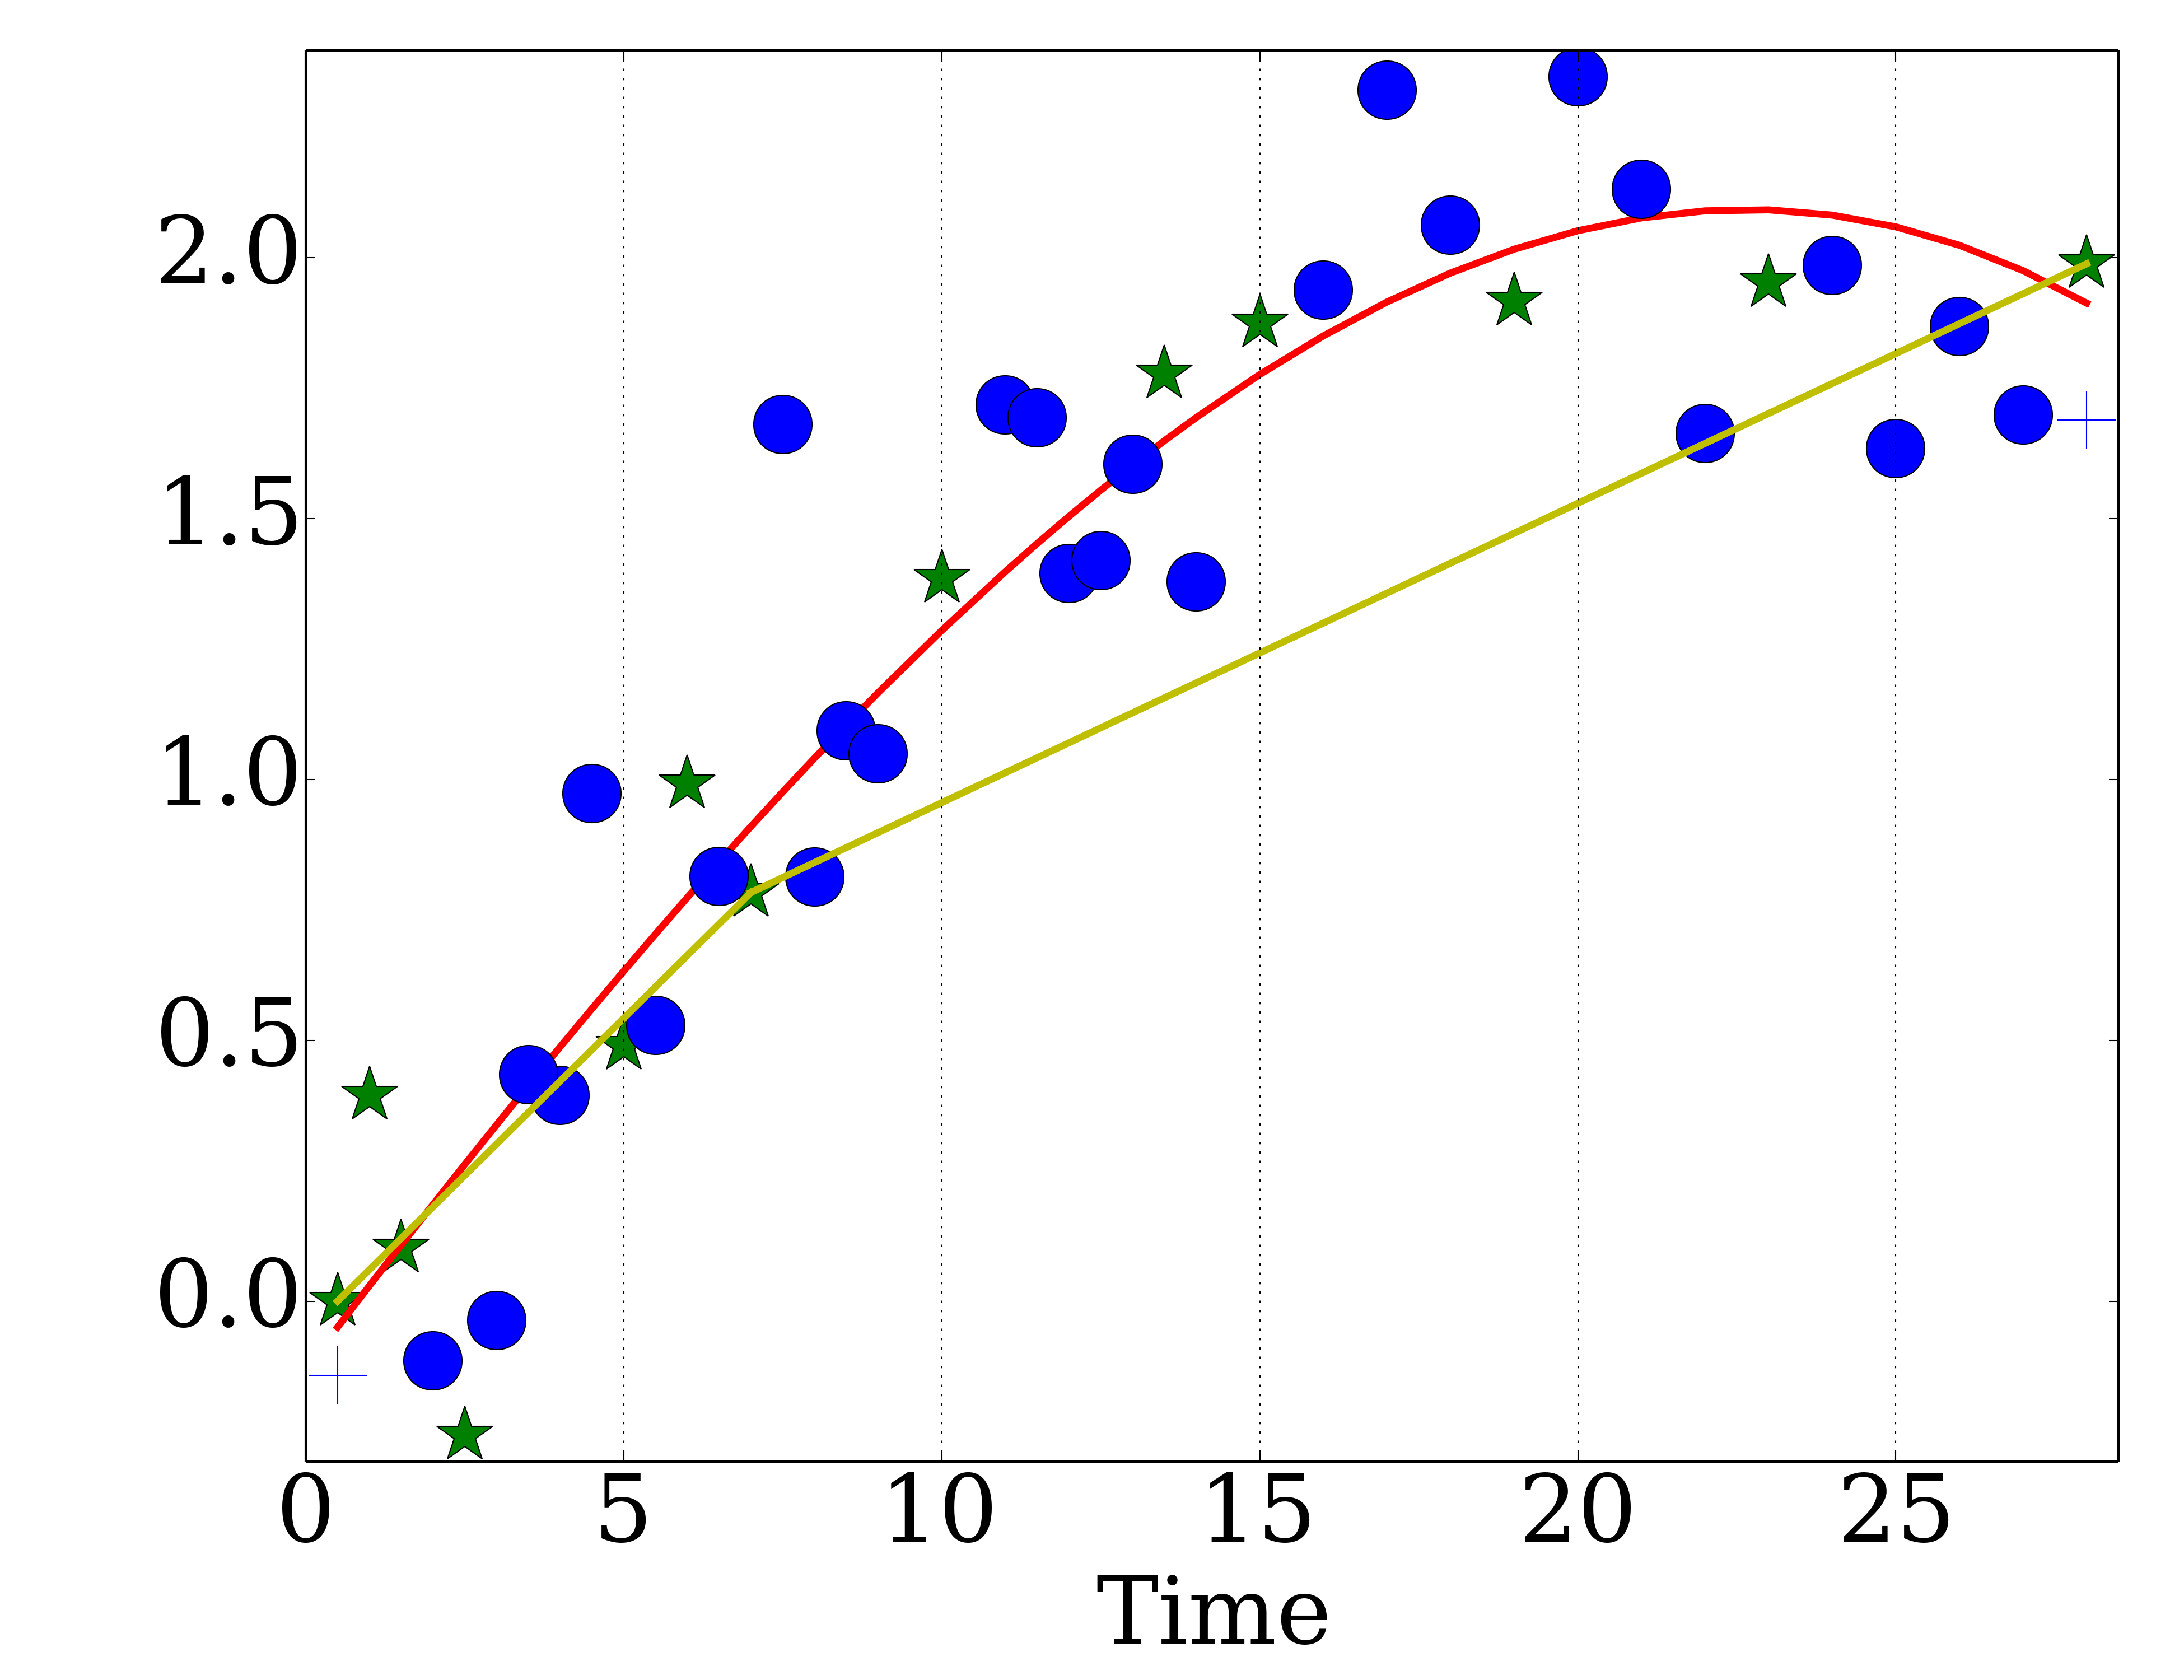
\includegraphics[scale=0.12]{{plots/newdata/splineAndLinear/17_PDGFRA_13_all}.png}}
\hfill
\subfloat[ELN]{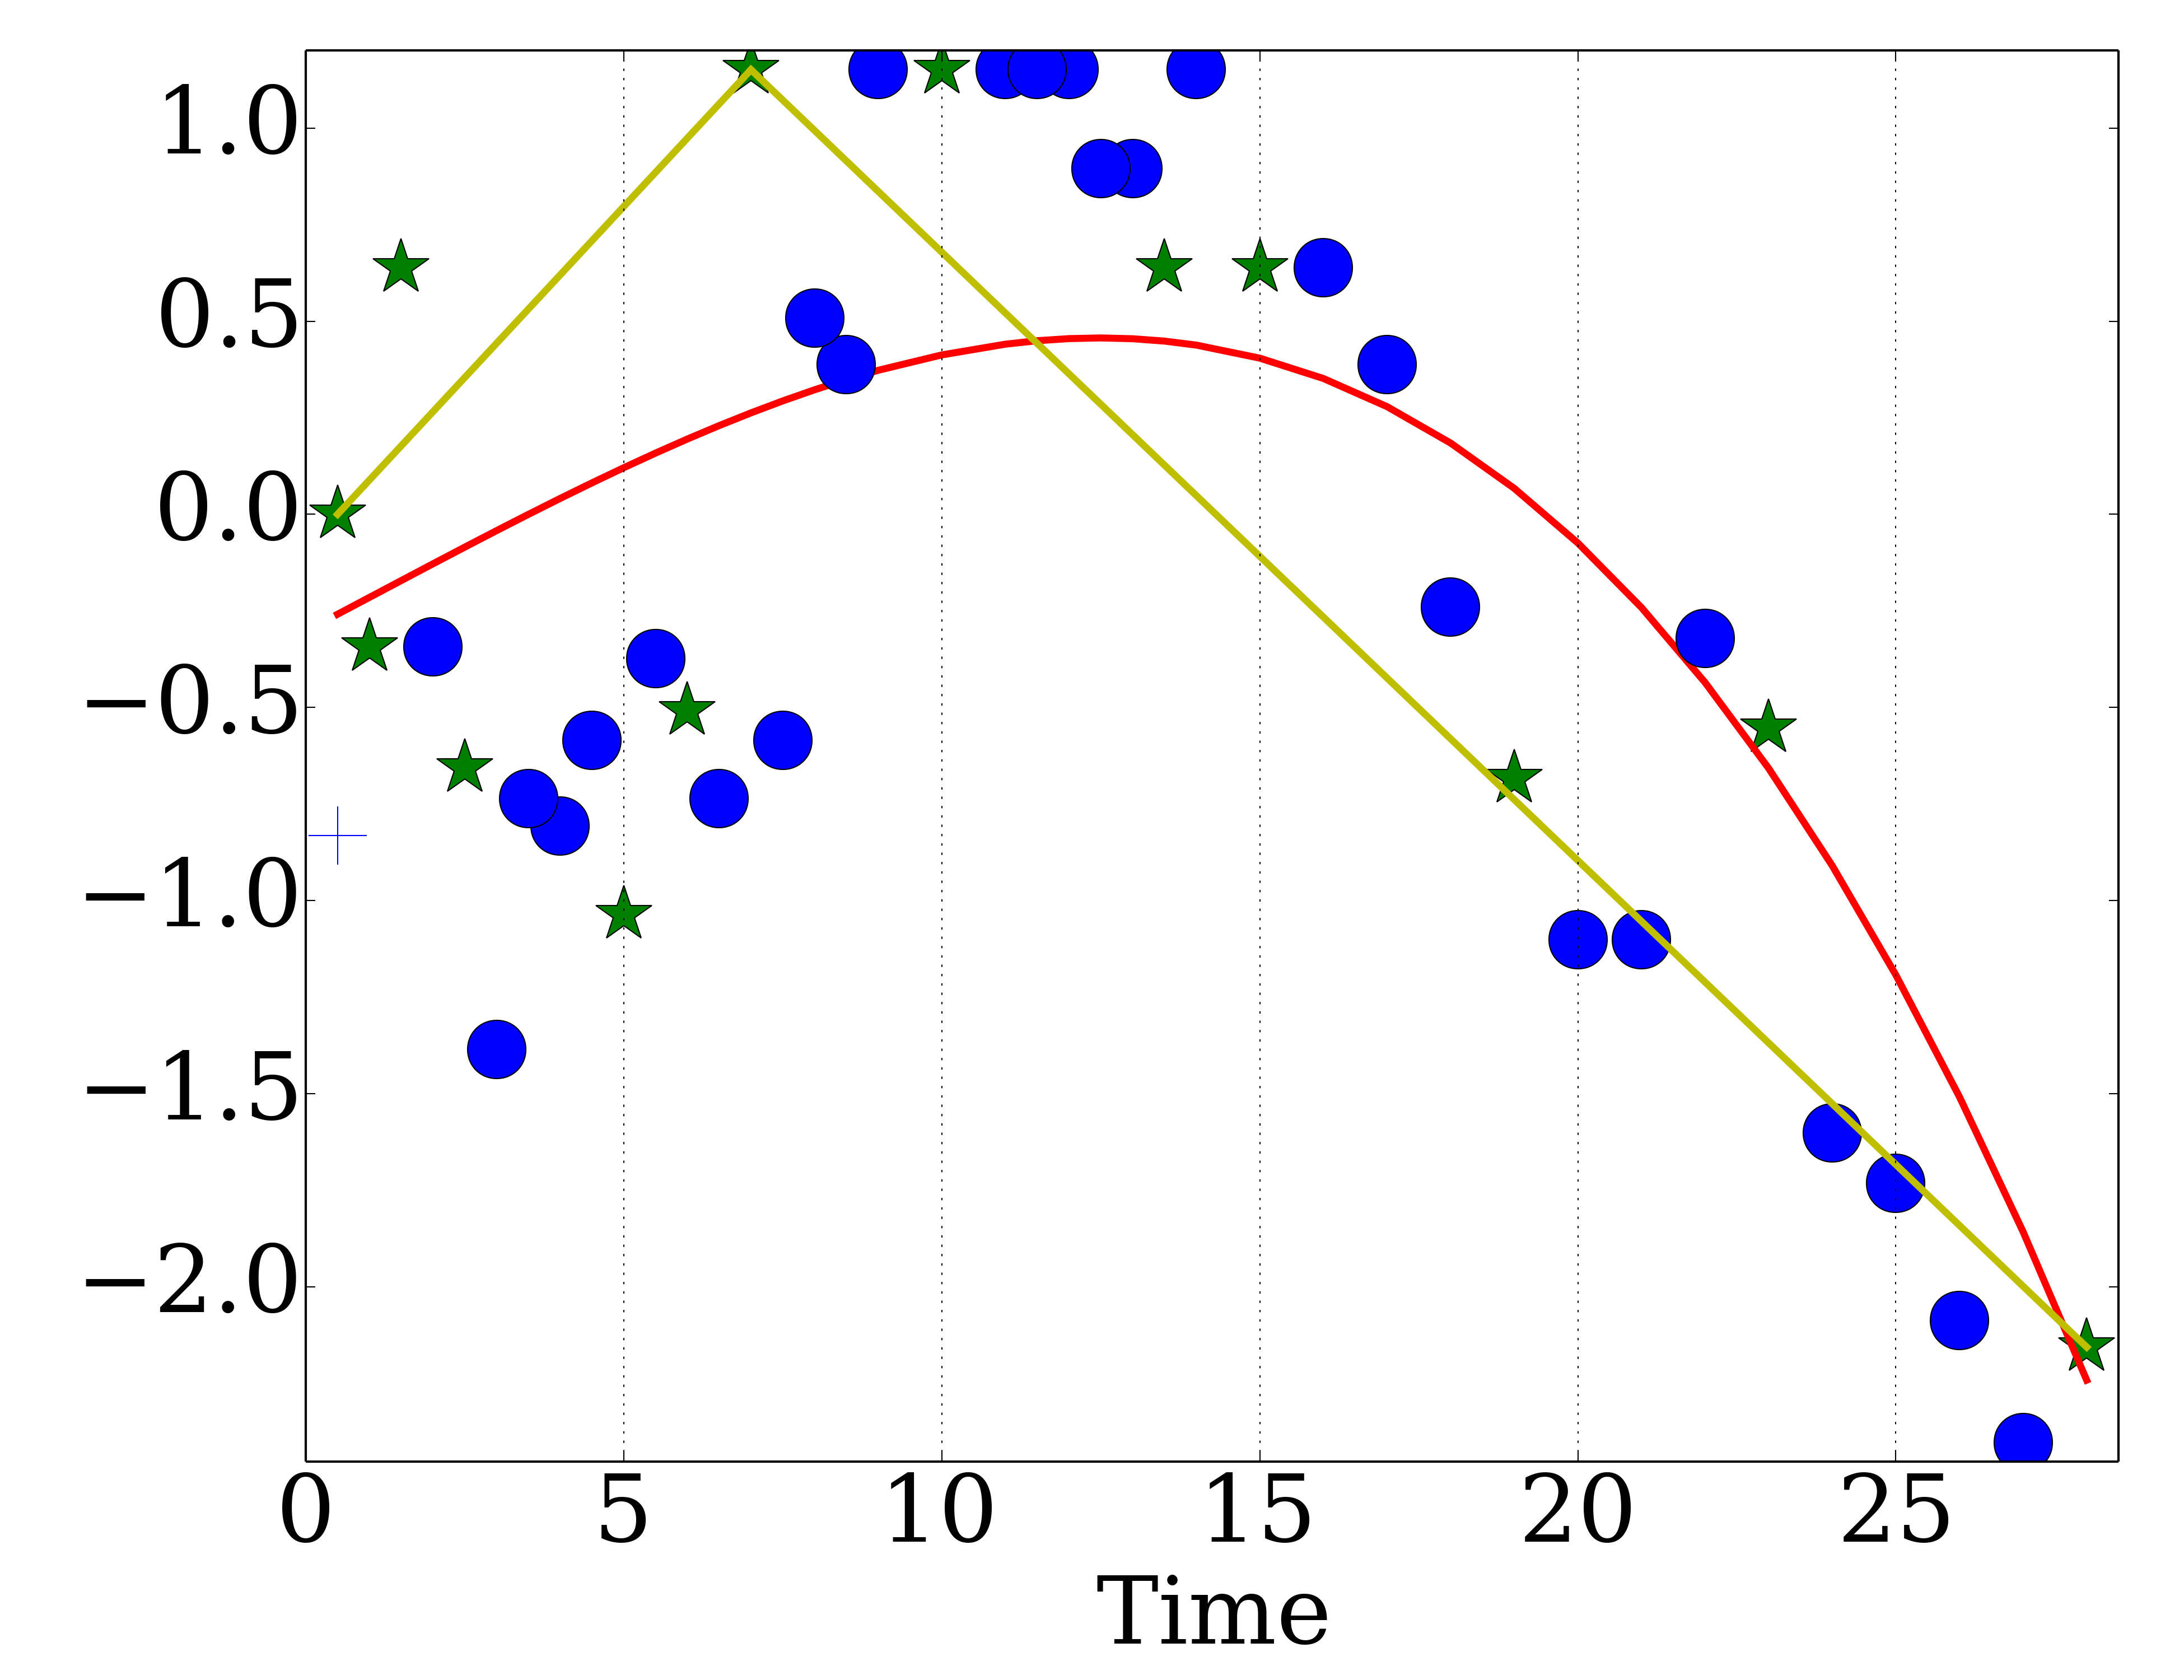
\includegraphics[scale=0.12]{{plots/newdata/splineAndLinear/14_Eln_13_all}.png}}
\hfill
\subfloat[LRAT]{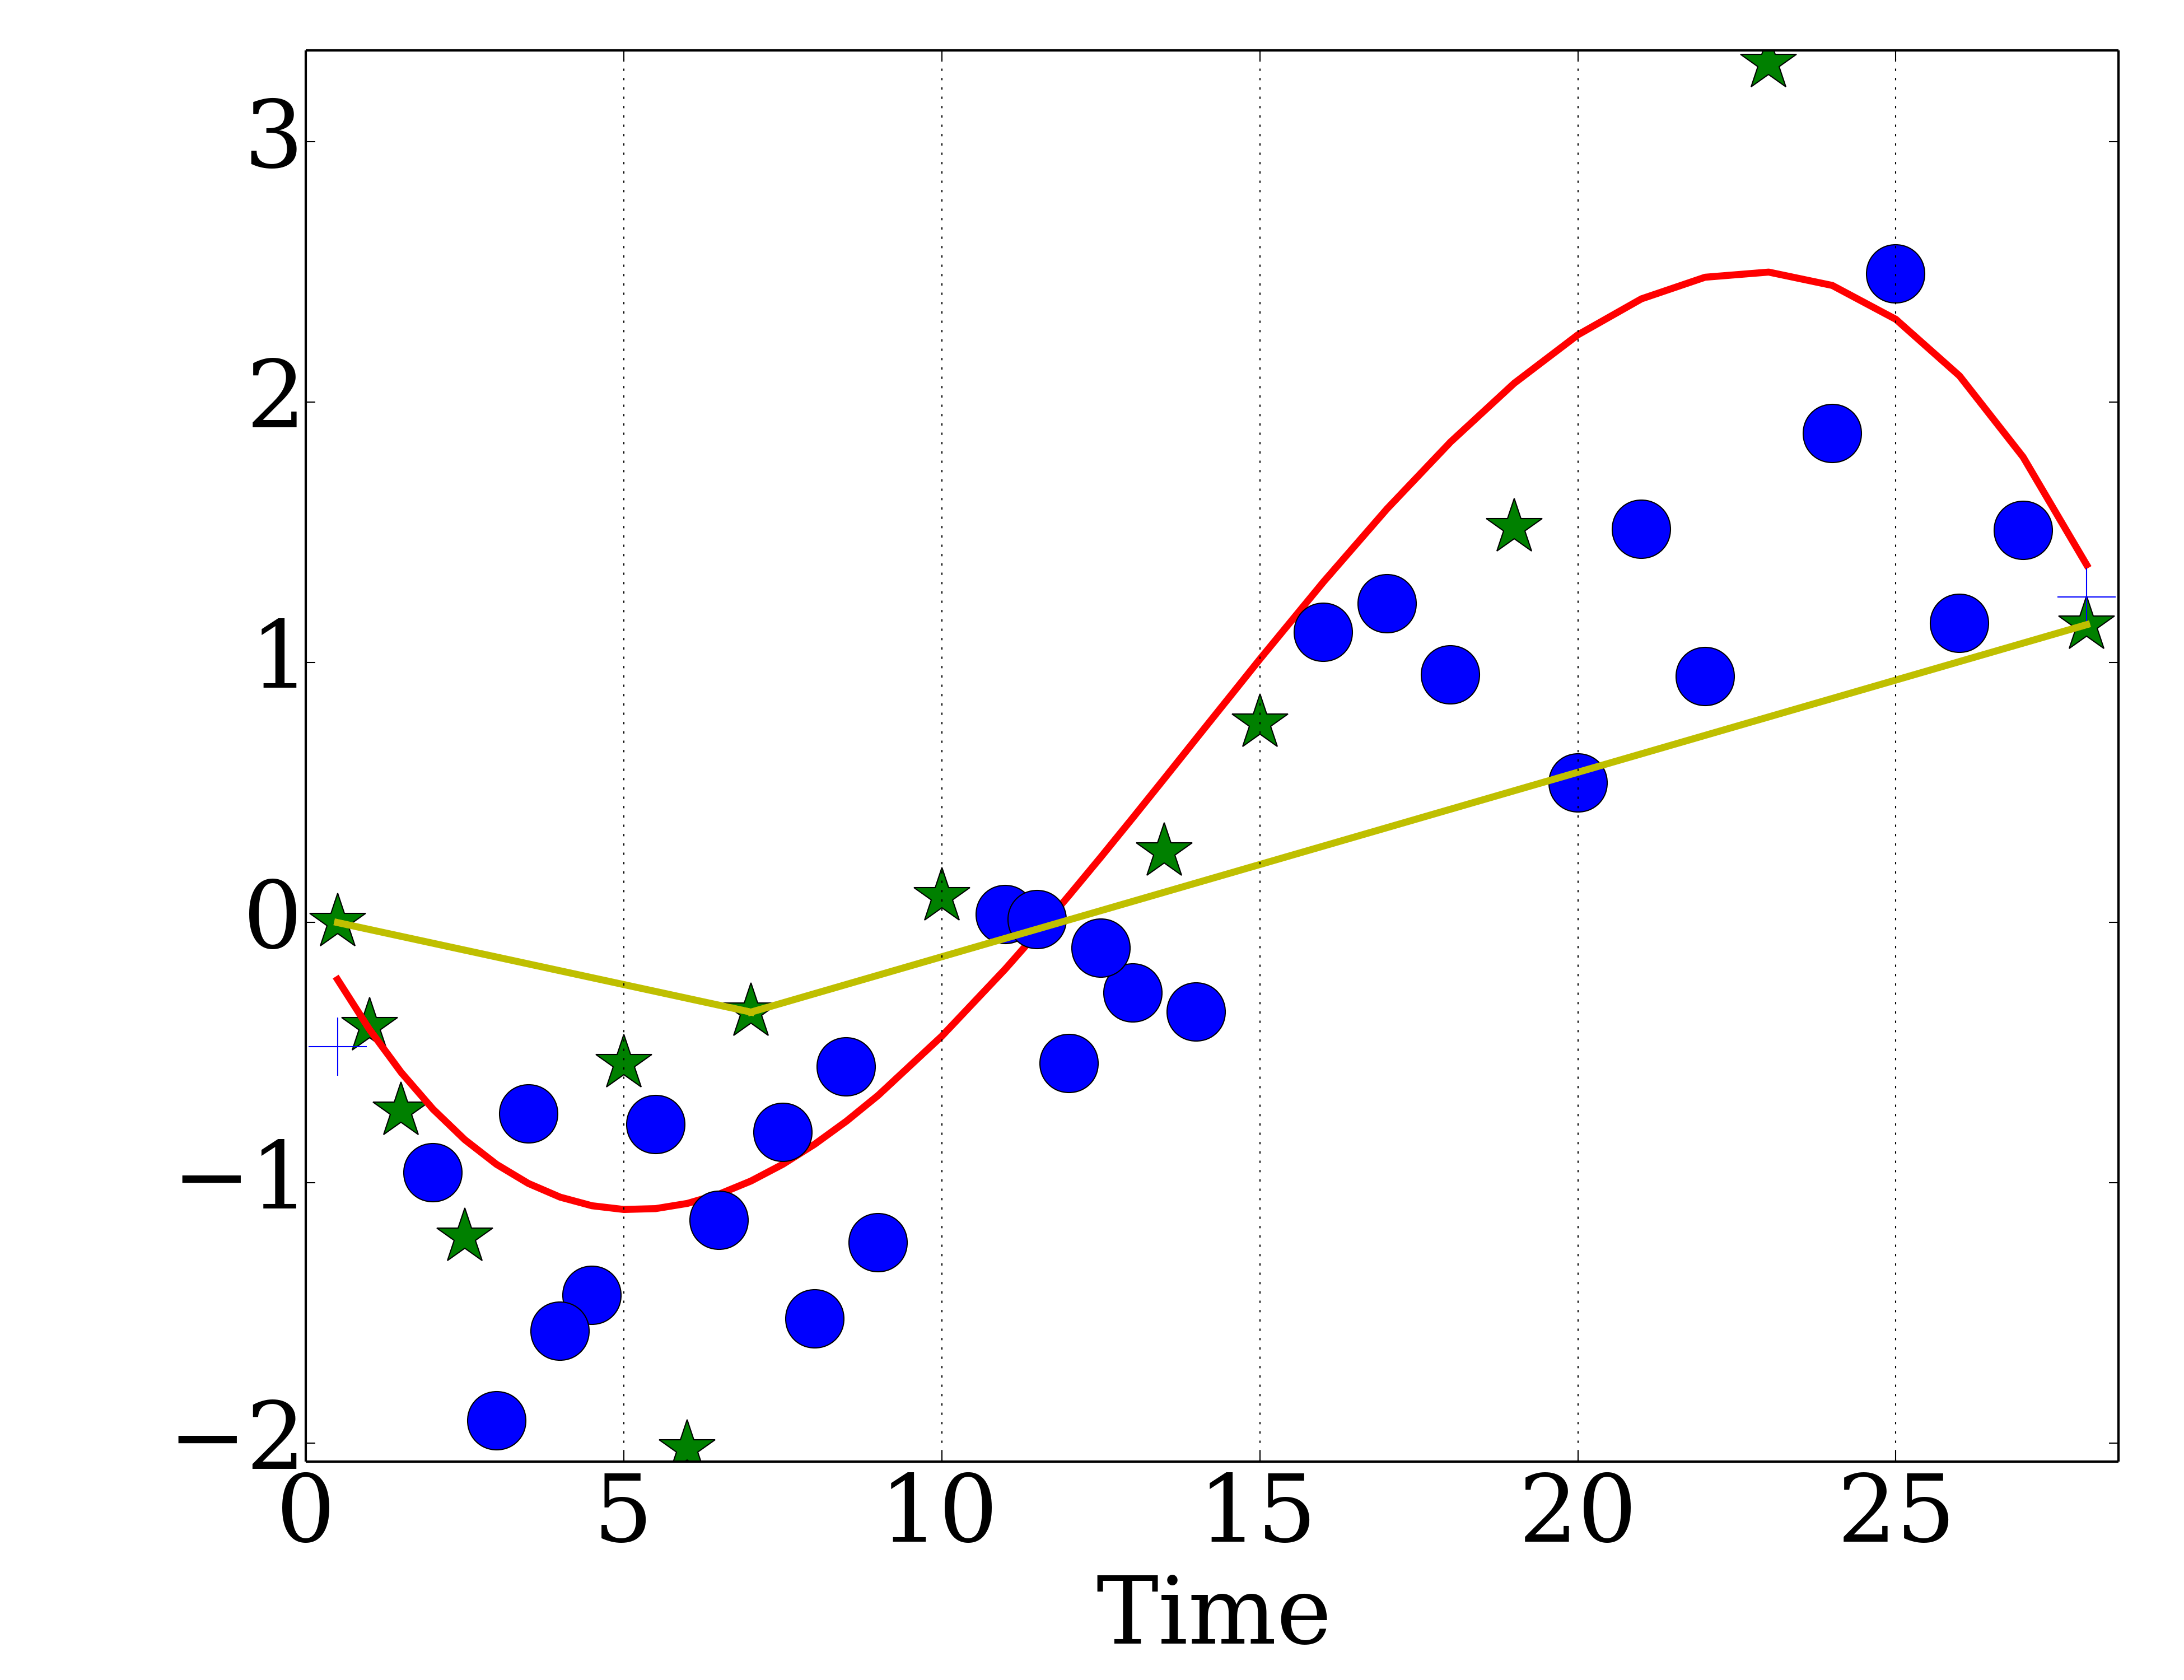
\includegraphics[scale=0.12]{{plots/newdata/splineAndLinear/1_LRAT_13_all}.png}}
\hfill
\end{minipage}
\caption{Comparison of \TPS and piecewise linear fitting over
  genes a) PDGFRA, b) ELN, c) LRAT}
\label{fig:sup5}
\end{figure}
\clearpage

\begin{figure}[ht]
\centering
\begin{minipage}{1.0\textwidth}
\subfloat[mmu-miR-100]{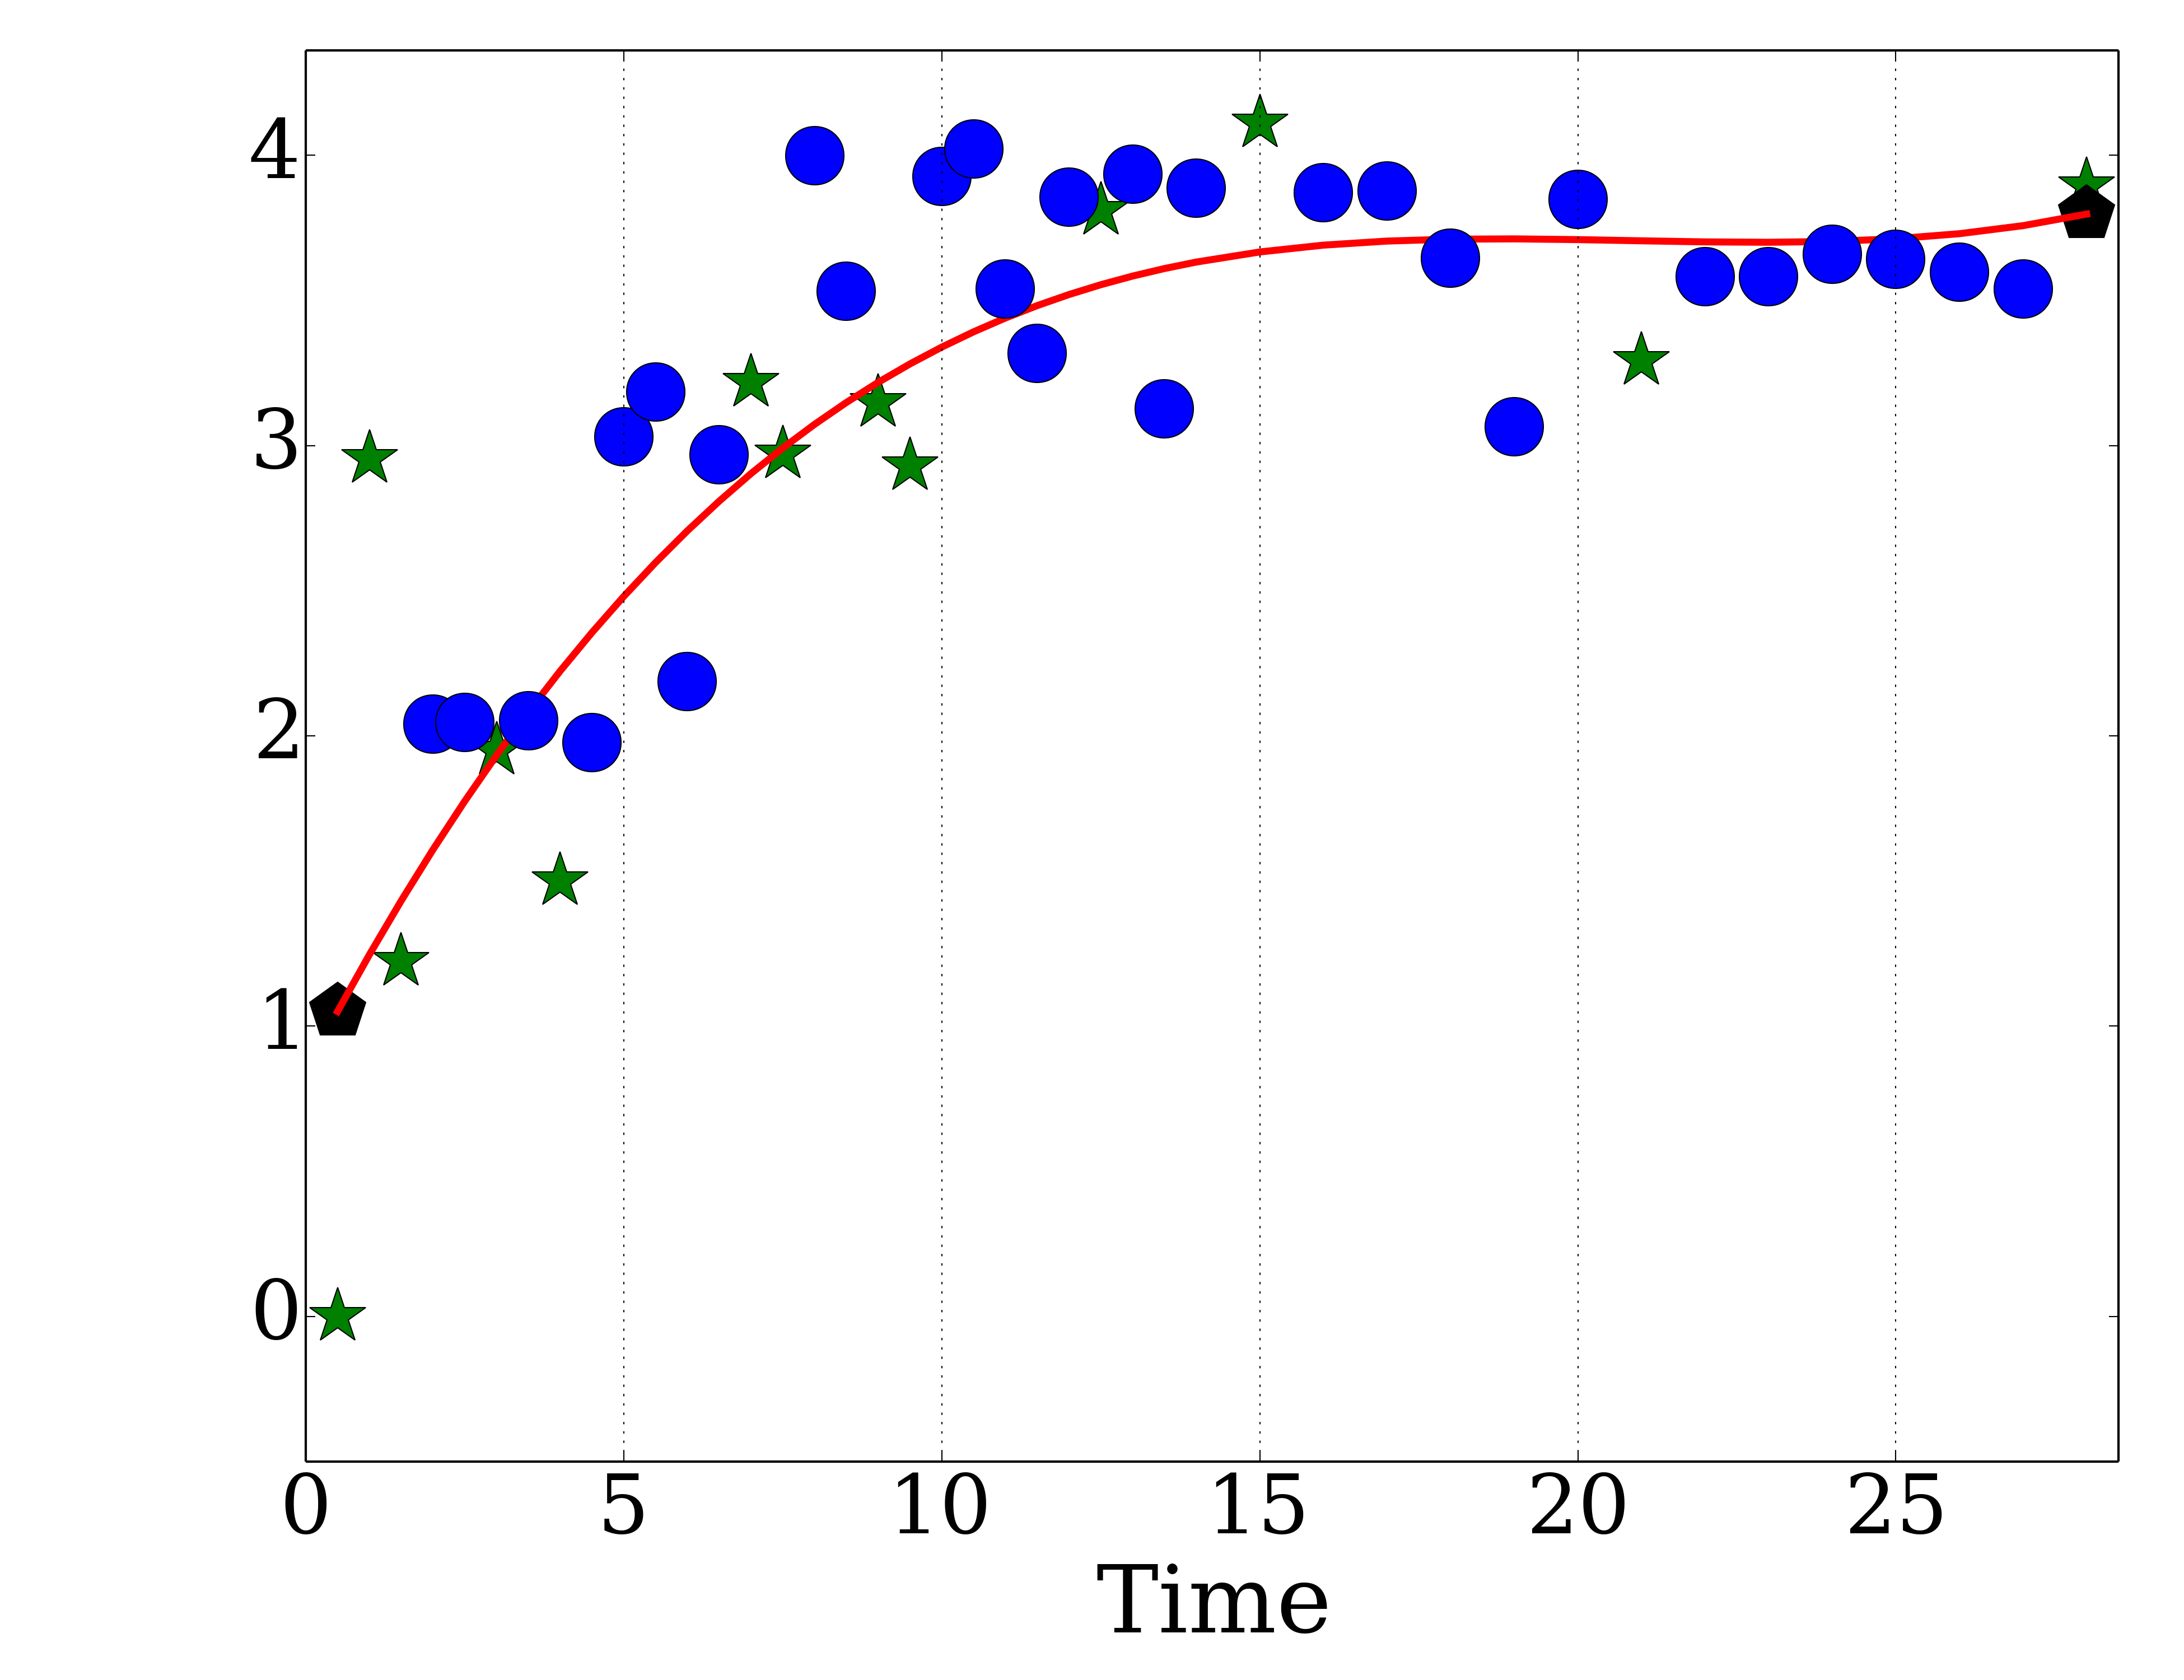
\includegraphics[scale=0.15]{{plots/mirnadata/splineplots13/uni/mmu-miR-100_13}.png}}
\hfill
\subfloat[mmu-miR-136]{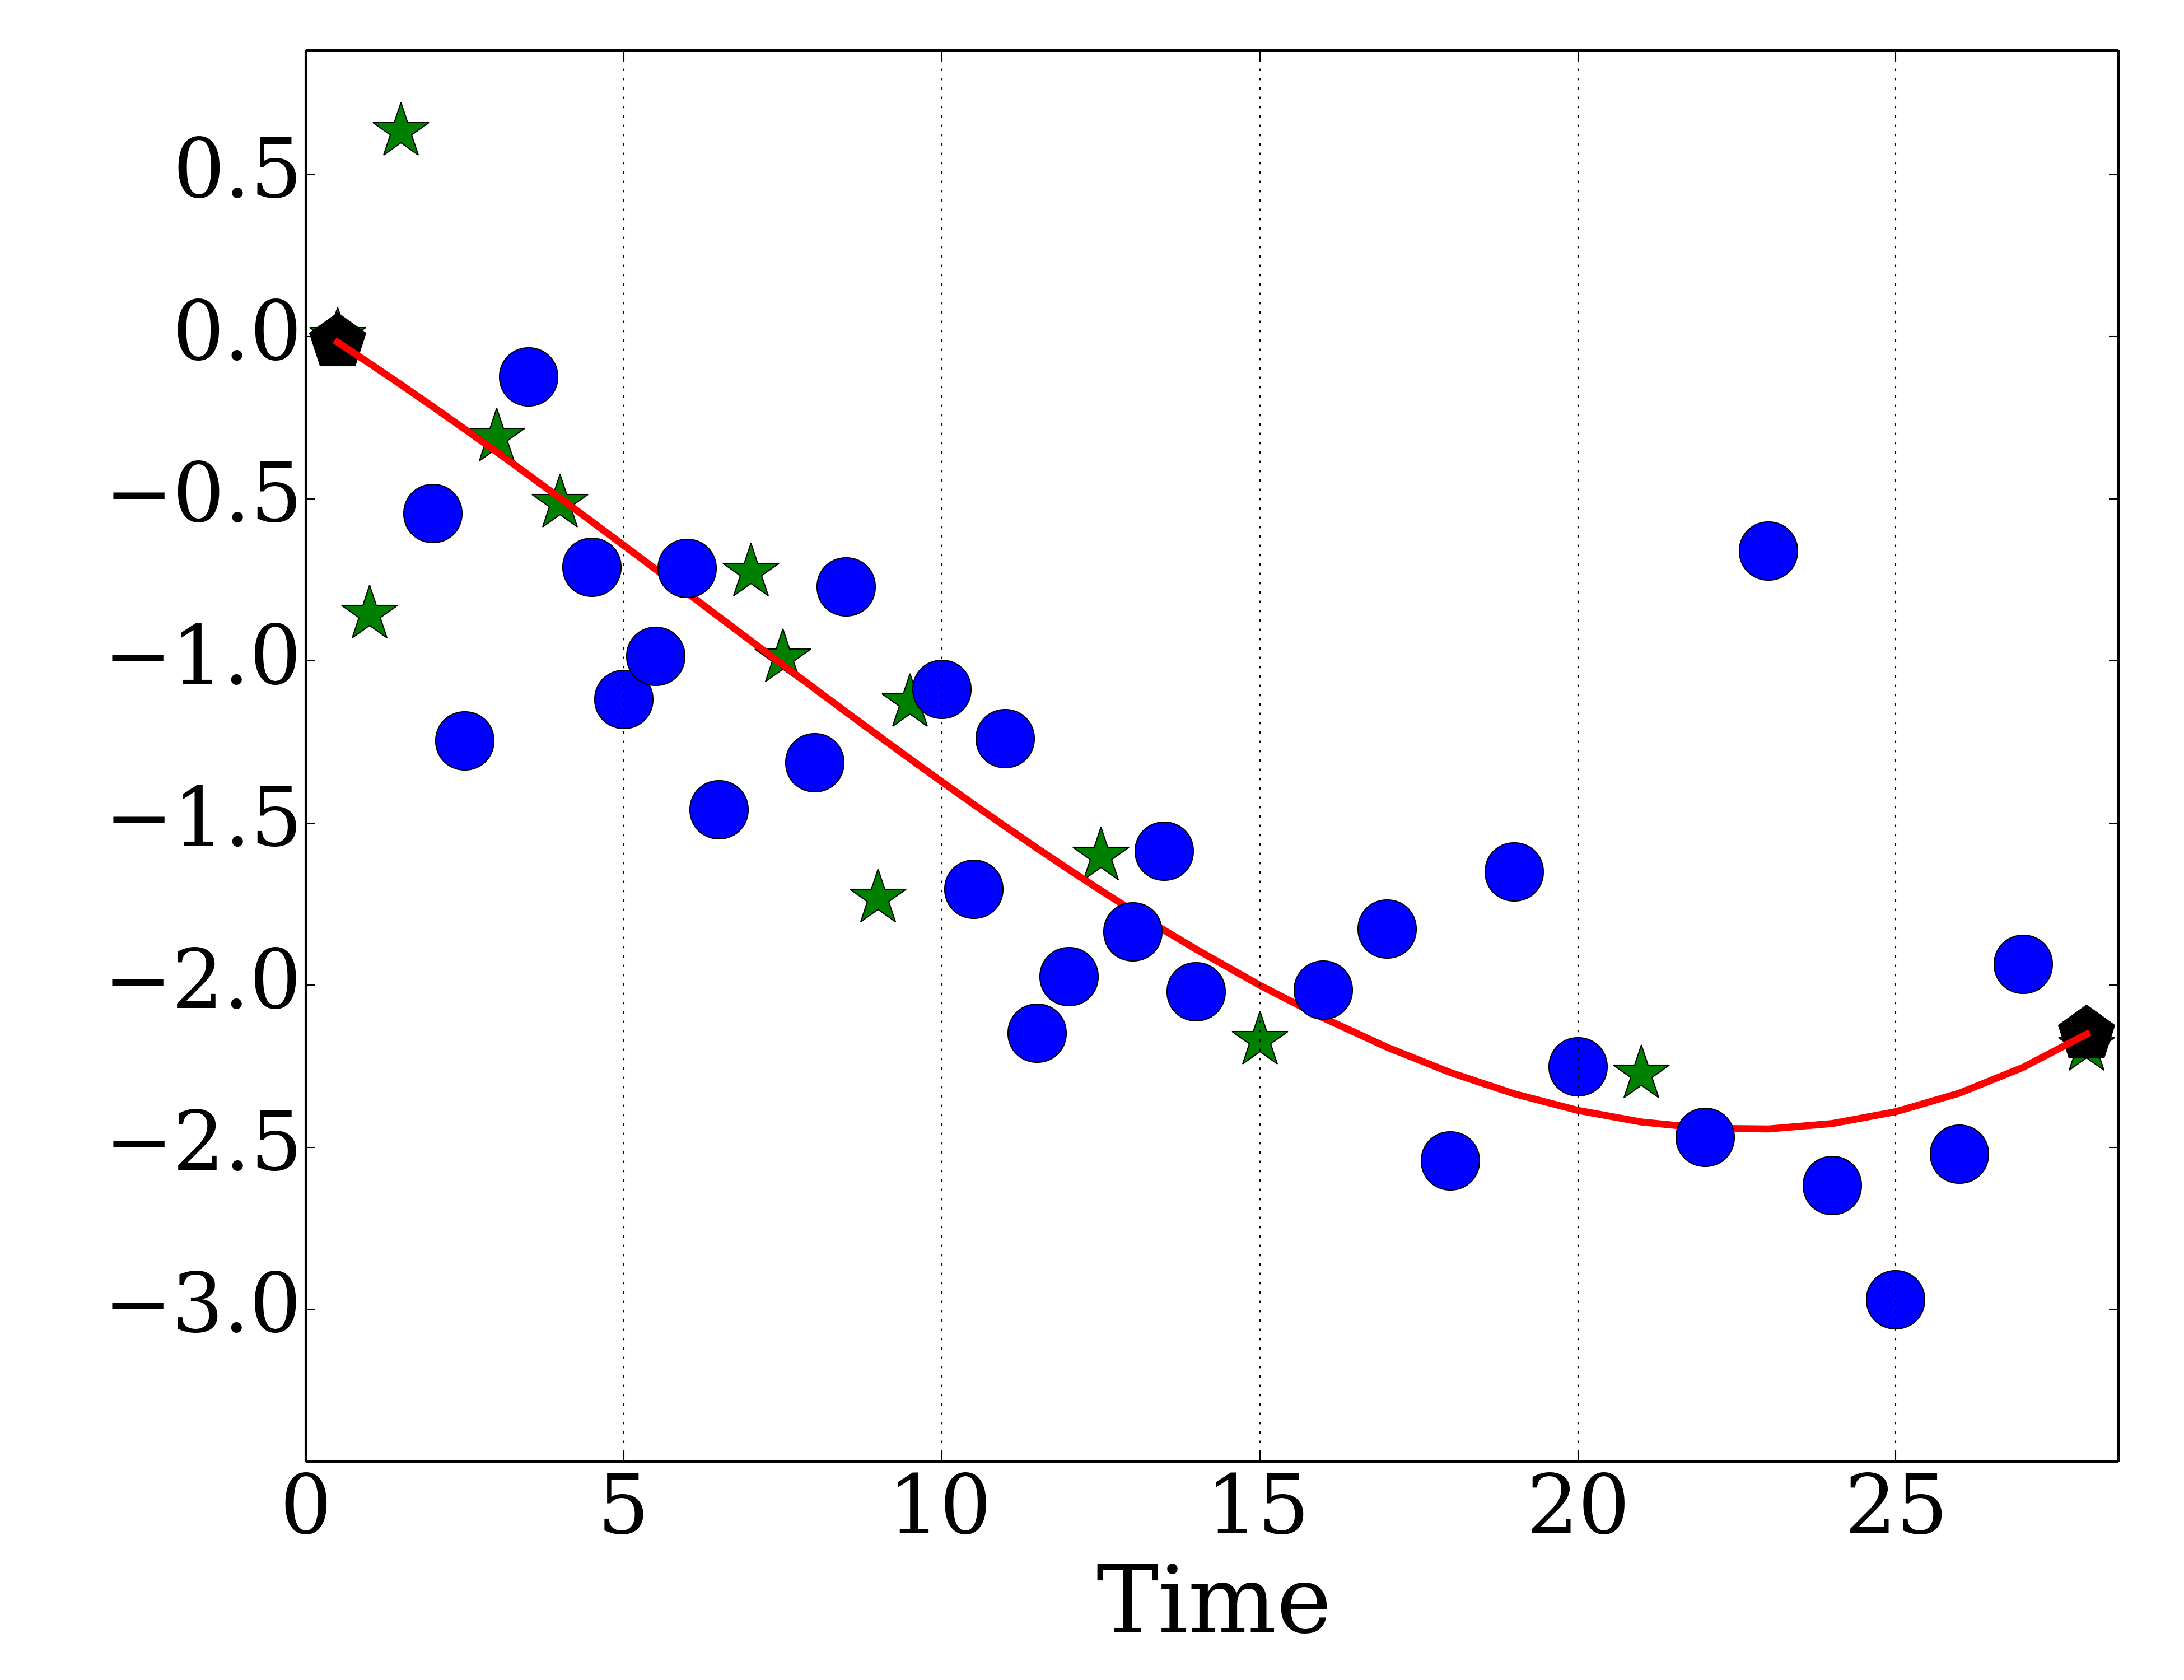
\includegraphics[scale=0.15]{{plots/mirnadata/splineplots13/uni/mmu-miR-136_13}.png}}
\\
\centering
\hfill
\subfloat[mmu-miR-152]{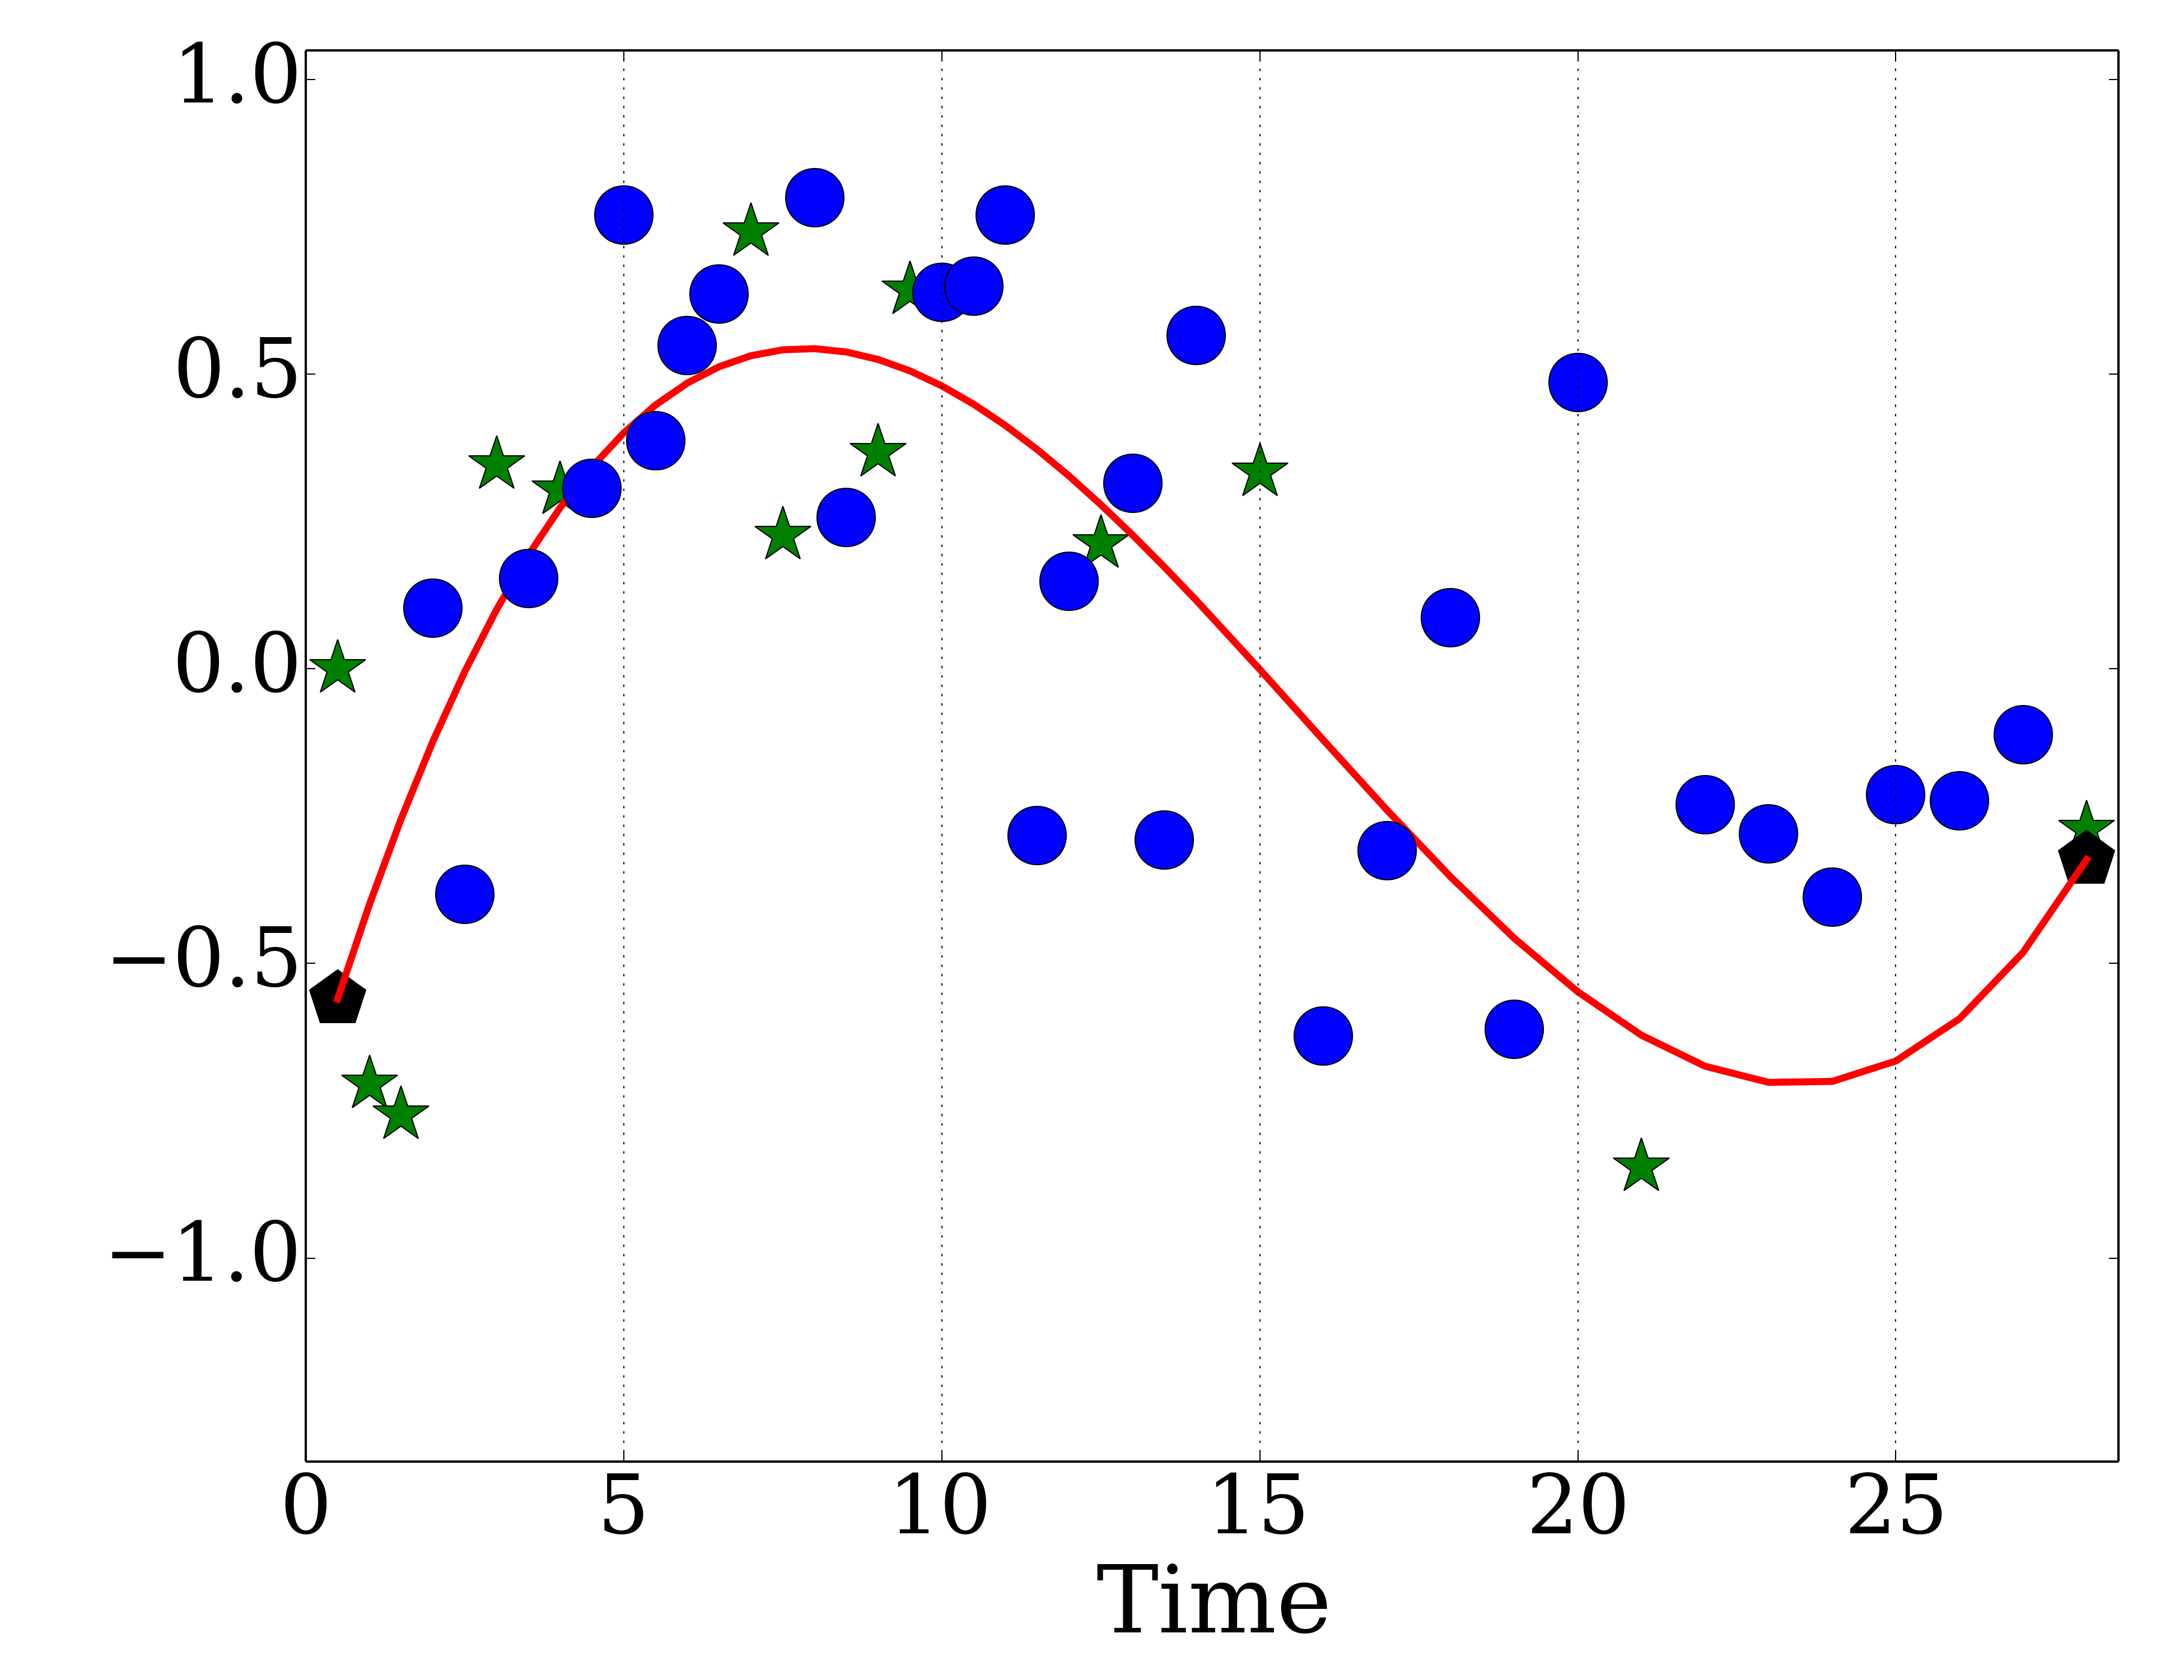
\includegraphics[scale=0.15]{{plots/mirnadata/splineplots13/uni/mmu-miR-152_13}.png}}
\hfill
\subfloat[mmu-miR-219]{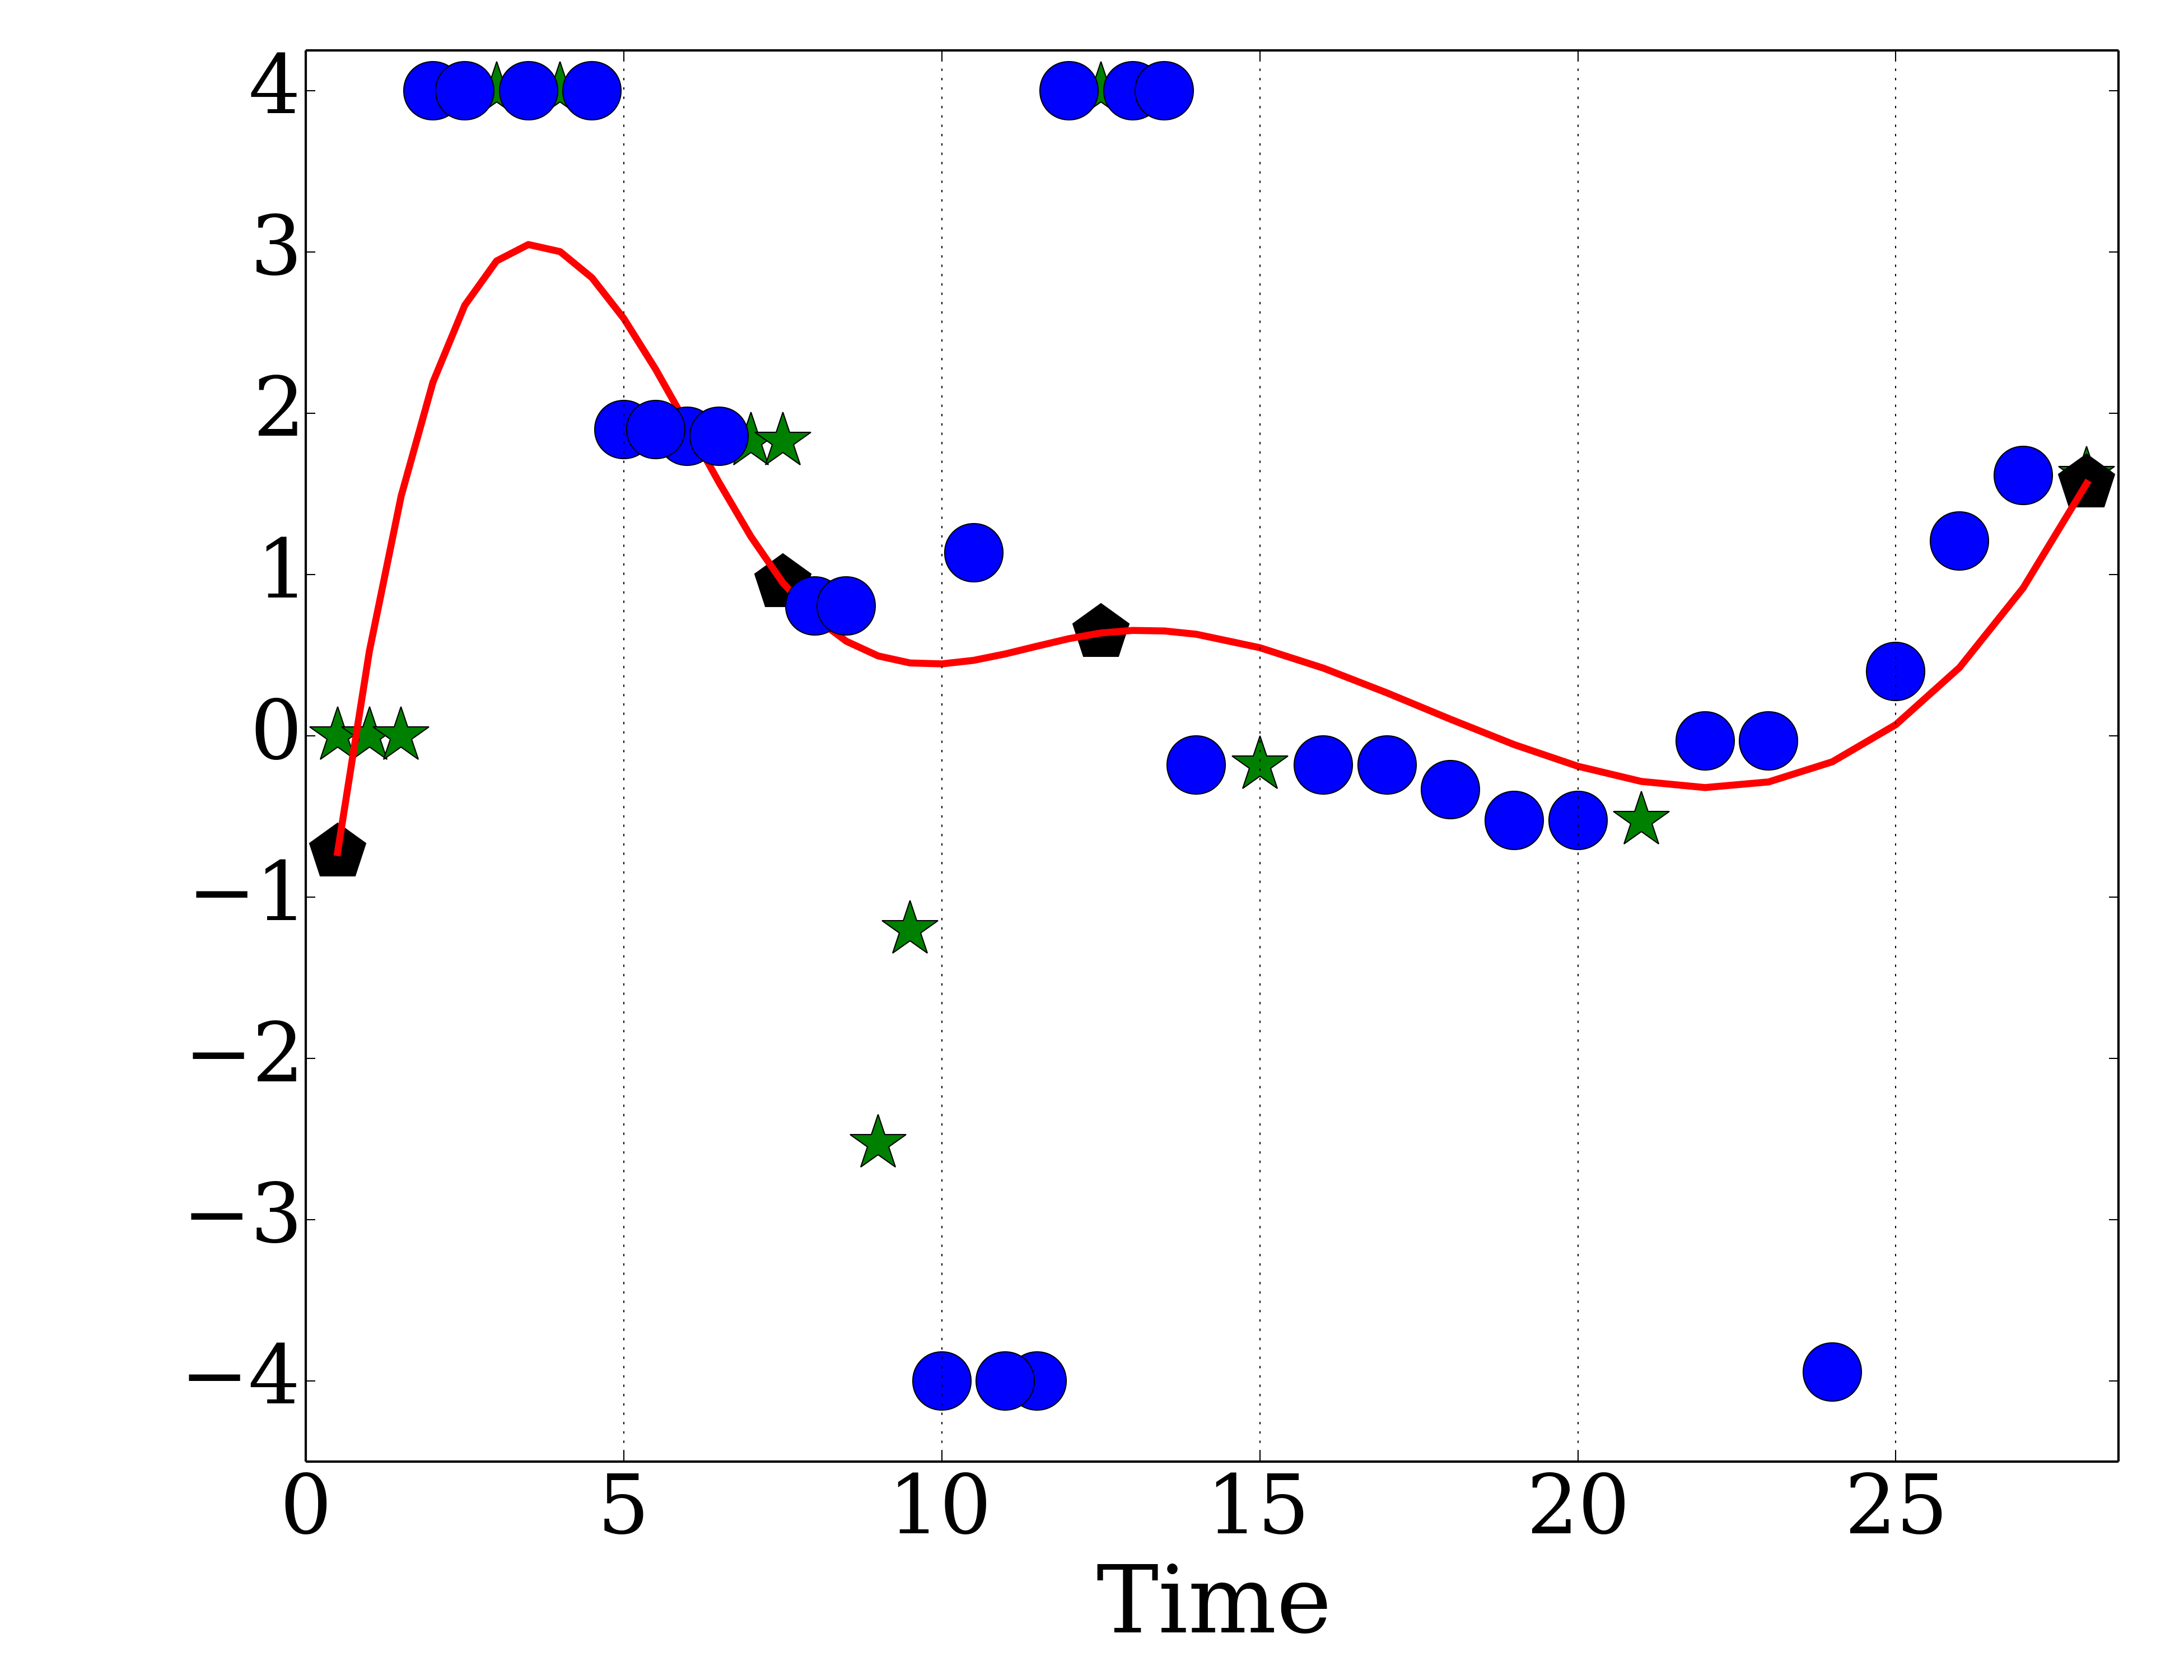
\includegraphics[scale=0.15]{{plots/mirnadata/splineplots13/uni/mmu-miR-219_13}.png}}
\end{minipage}
\caption{Predicted expression profiles of miRNAs a) mmu-miR-100, b)
  mmu-miR-136, c) mmu-miR-152, d) mmu-miR-219.}
\label{fig:mirnaplots_spec}
\end{figure}
\clearpage

\begin{figure}
\centering
\begin{minipage}{1.0\textwidth}
\subfloat[Chromo~2, 157423995 (SRC)]{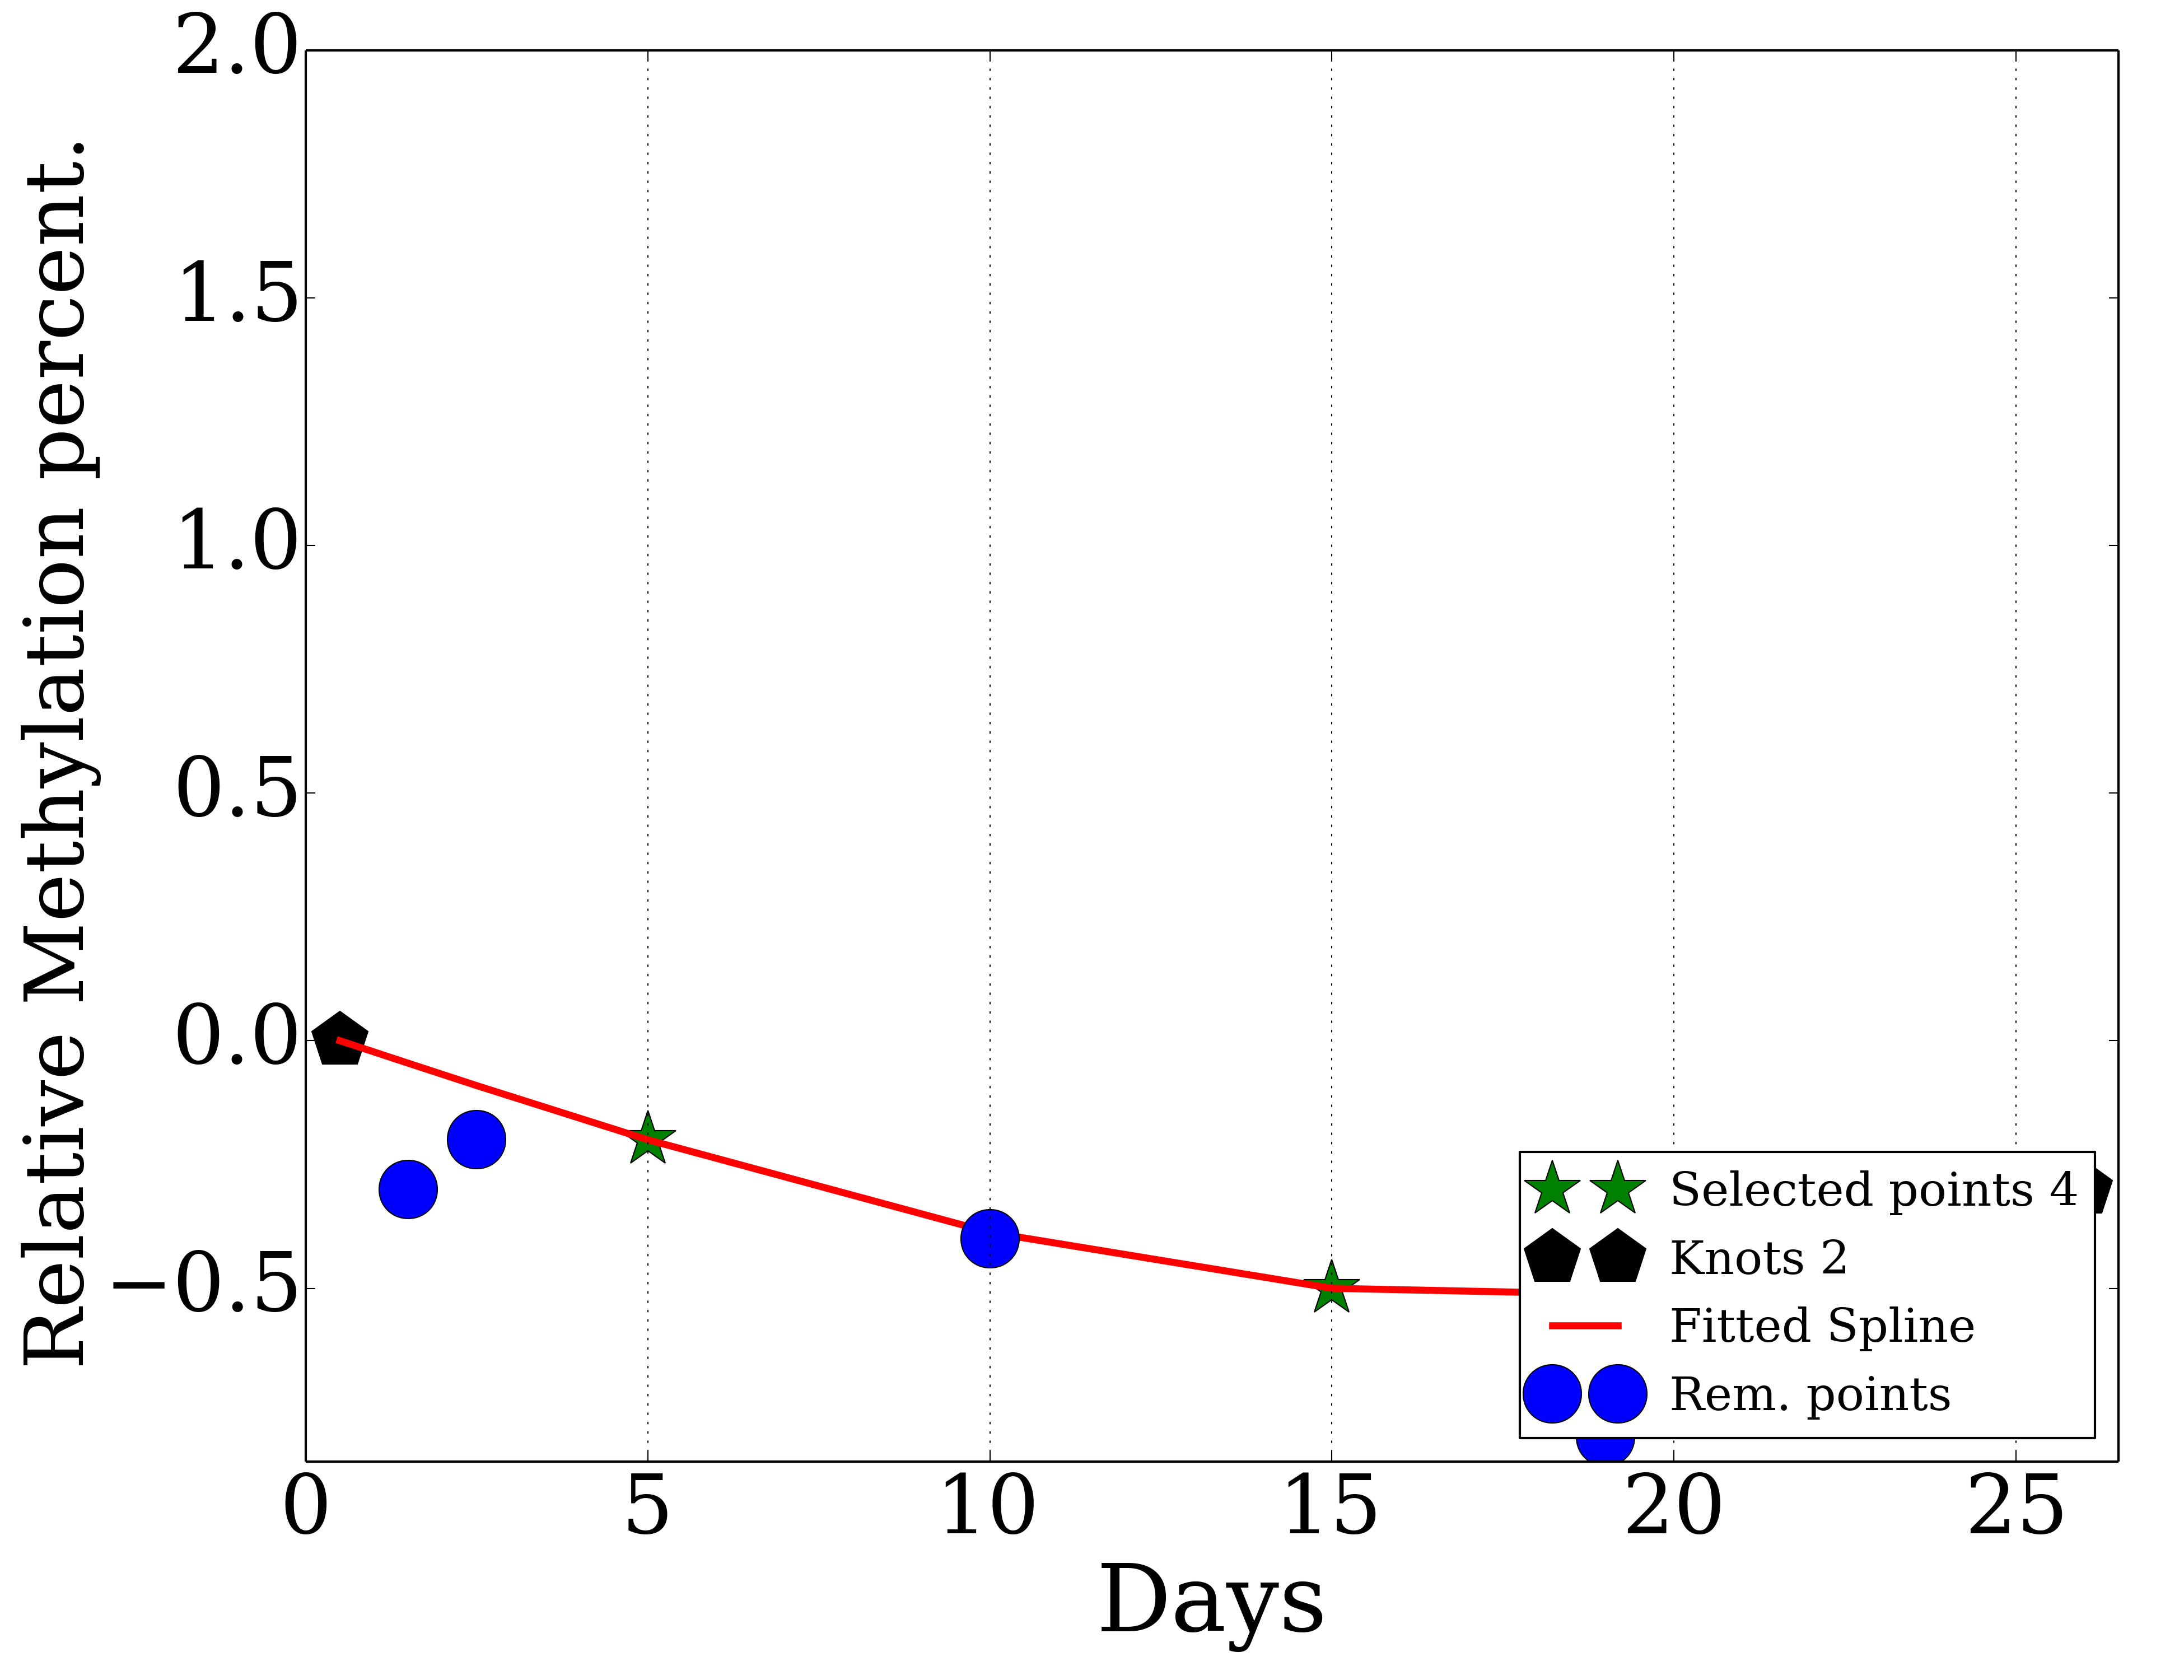
\includegraphics[scale=0.11]{{plots/meth/splineplots/uni/chr2__157423995_4}.png}}
\hfill
\subfloat[Chrom.~5, 134721315 (ELN)]{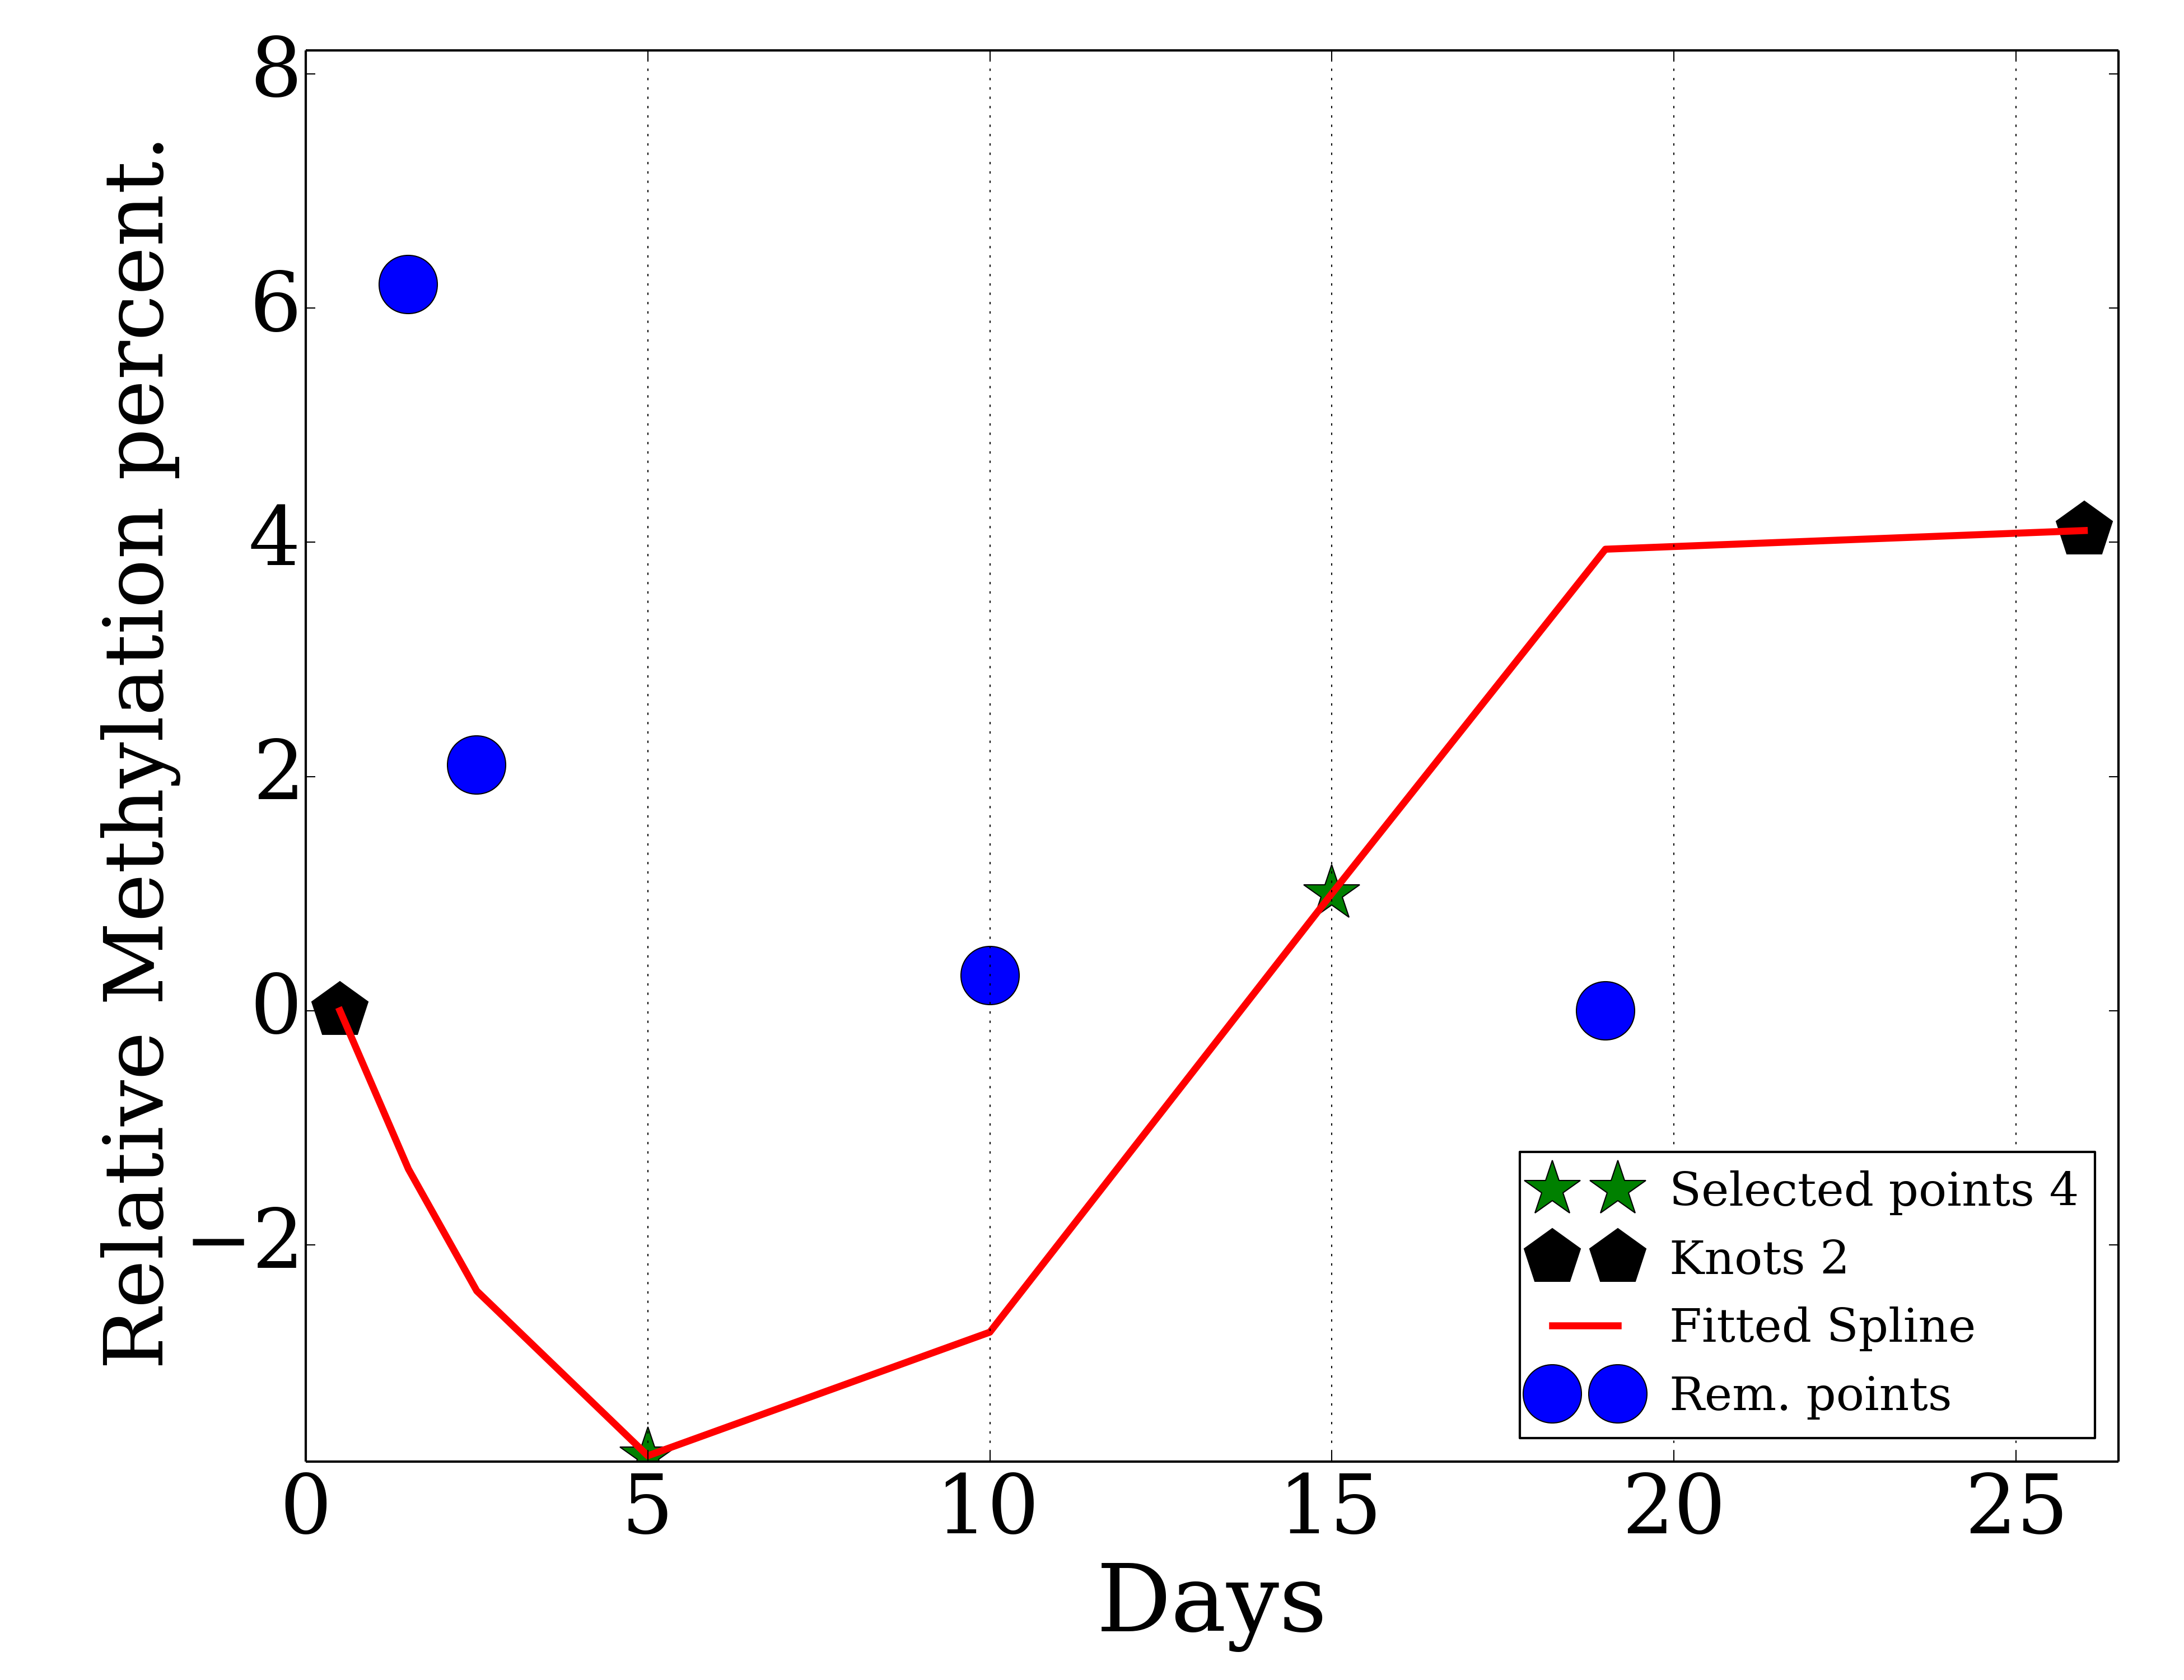
\includegraphics[scale=0.11]{{plots/meth/splineplots/uni/chr5__134721315_4}.png}}
\hfill
\subfloat[Chrom.~12, 112657170 (AKT1)]{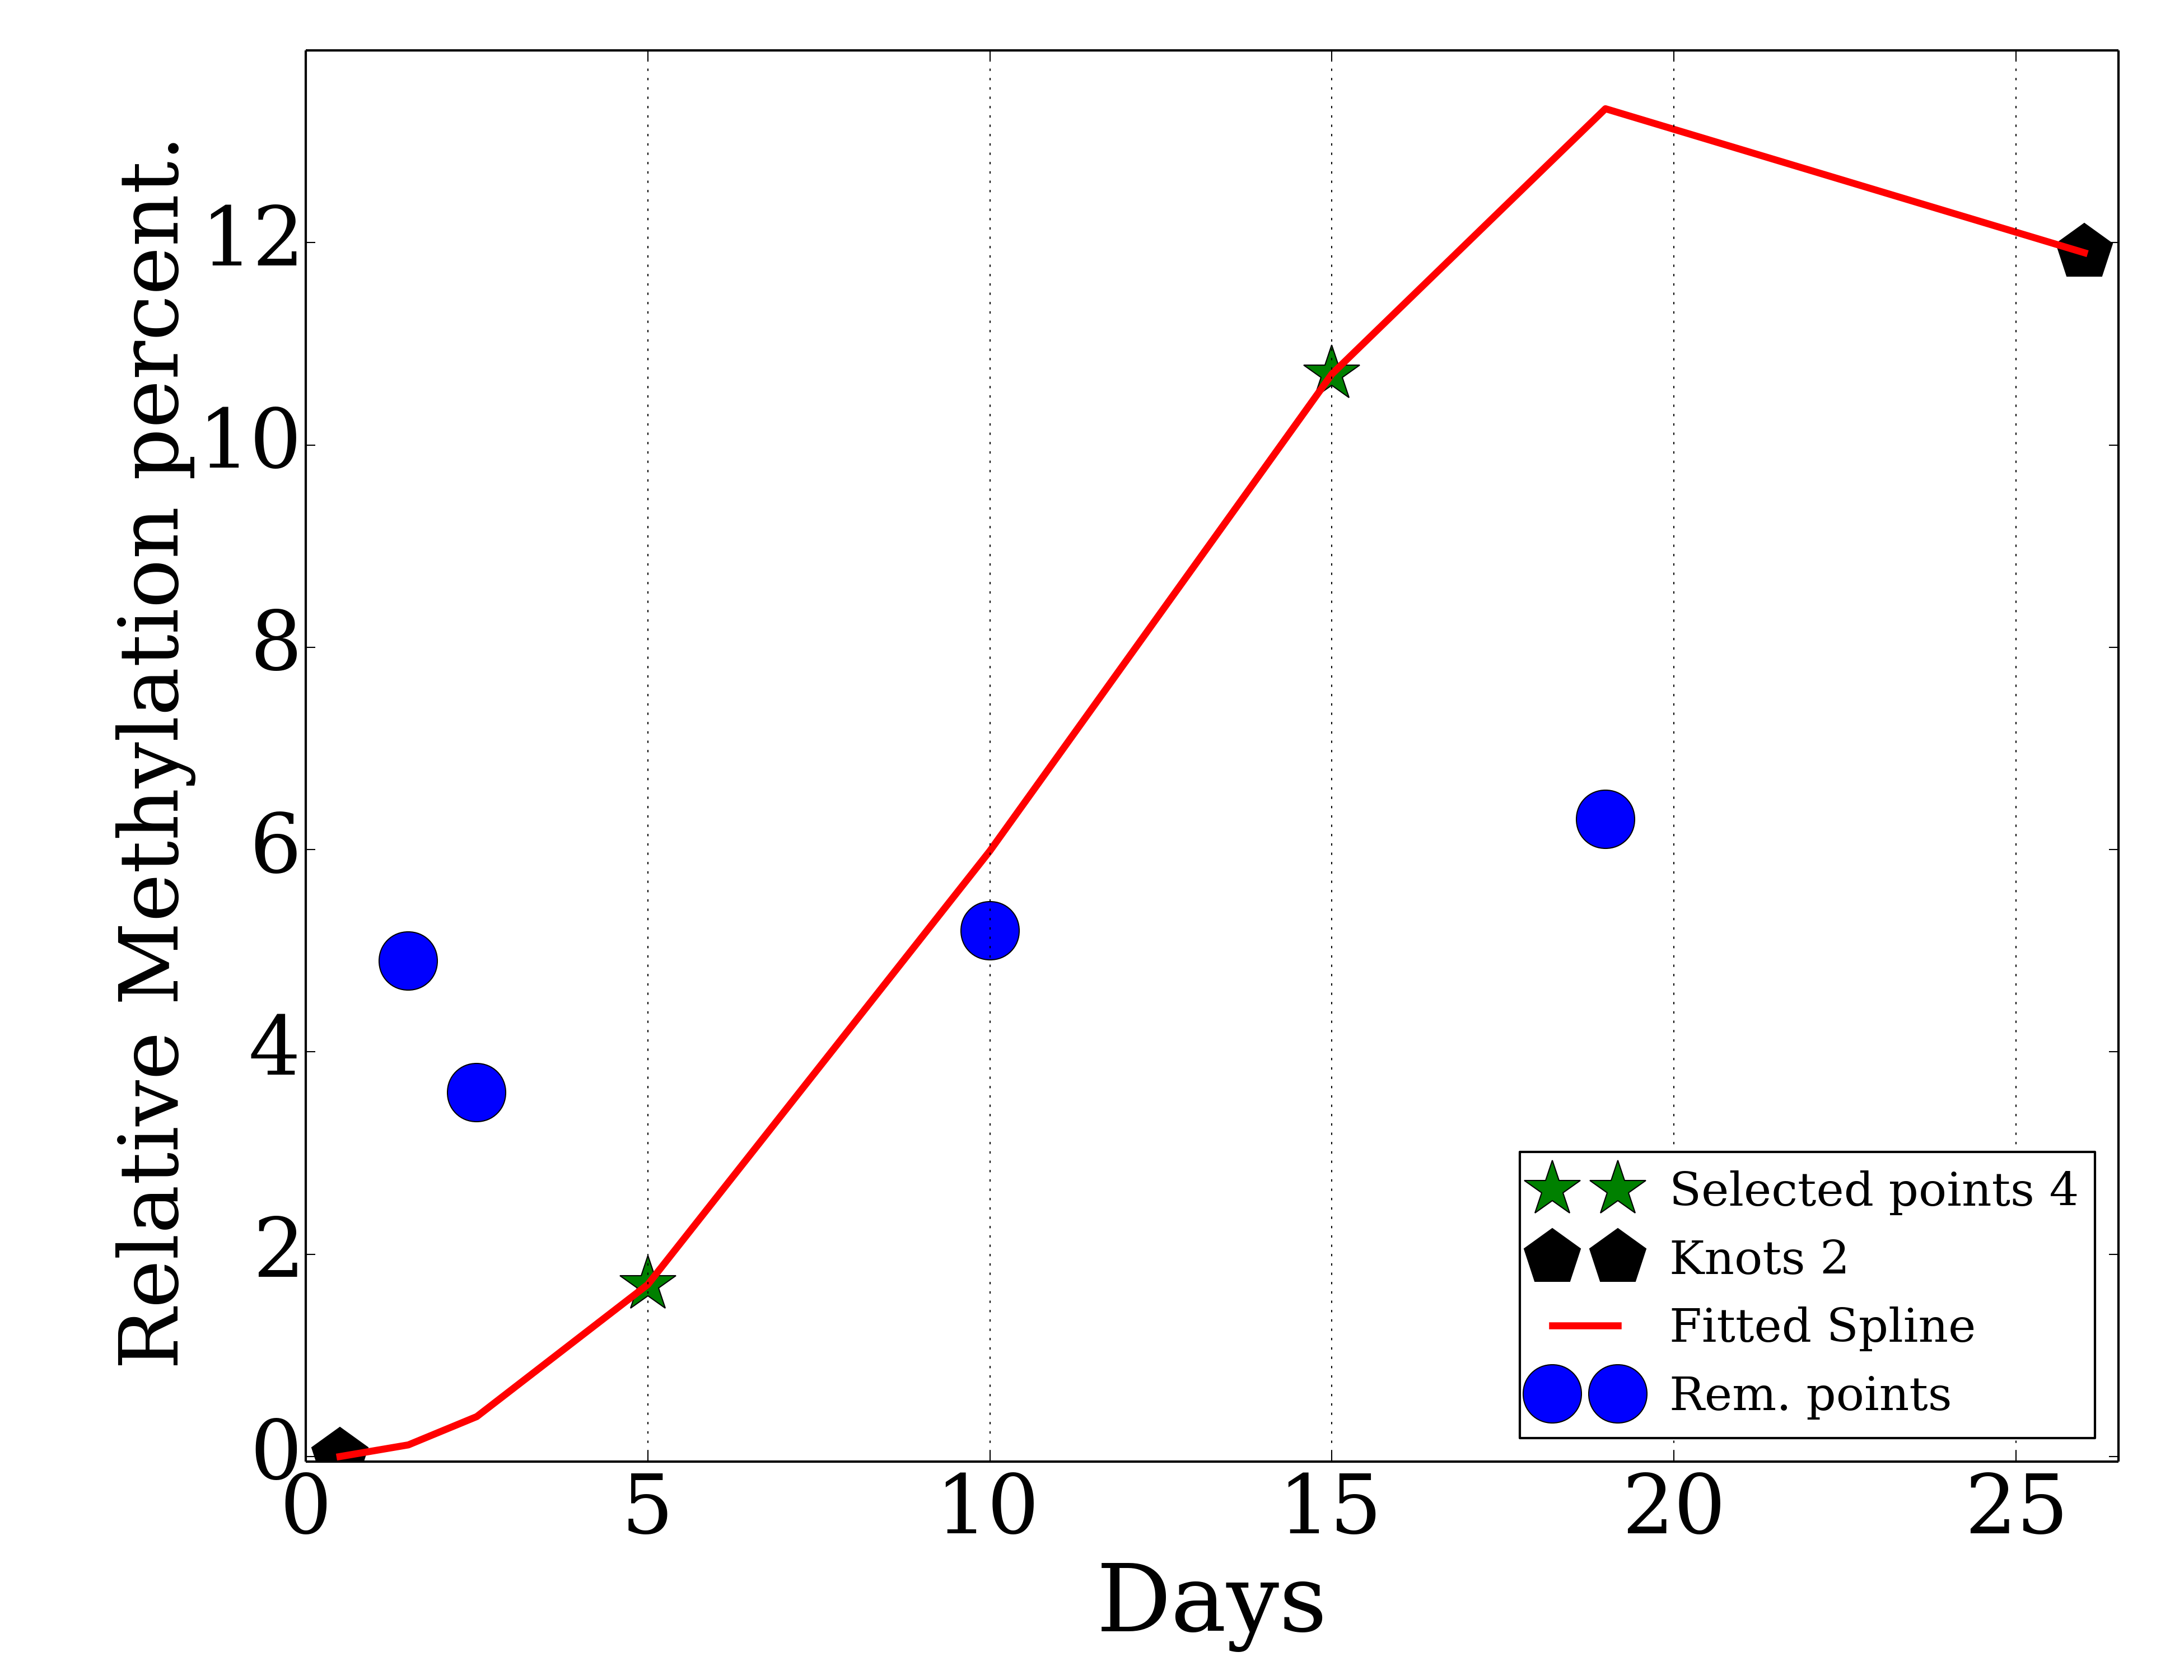
\includegraphics[scale=0.11]{{plots/meth/splineplots/uni/chr12__112657170_4}.png}}
\end{minipage}
\caption{Reconstructed methylation profiles over several
  loci~(chromosome, position) with corresponding genes.}
\label{fig:methpredict}
\end{figure}
\clearpage

\begin{figure}
\centering
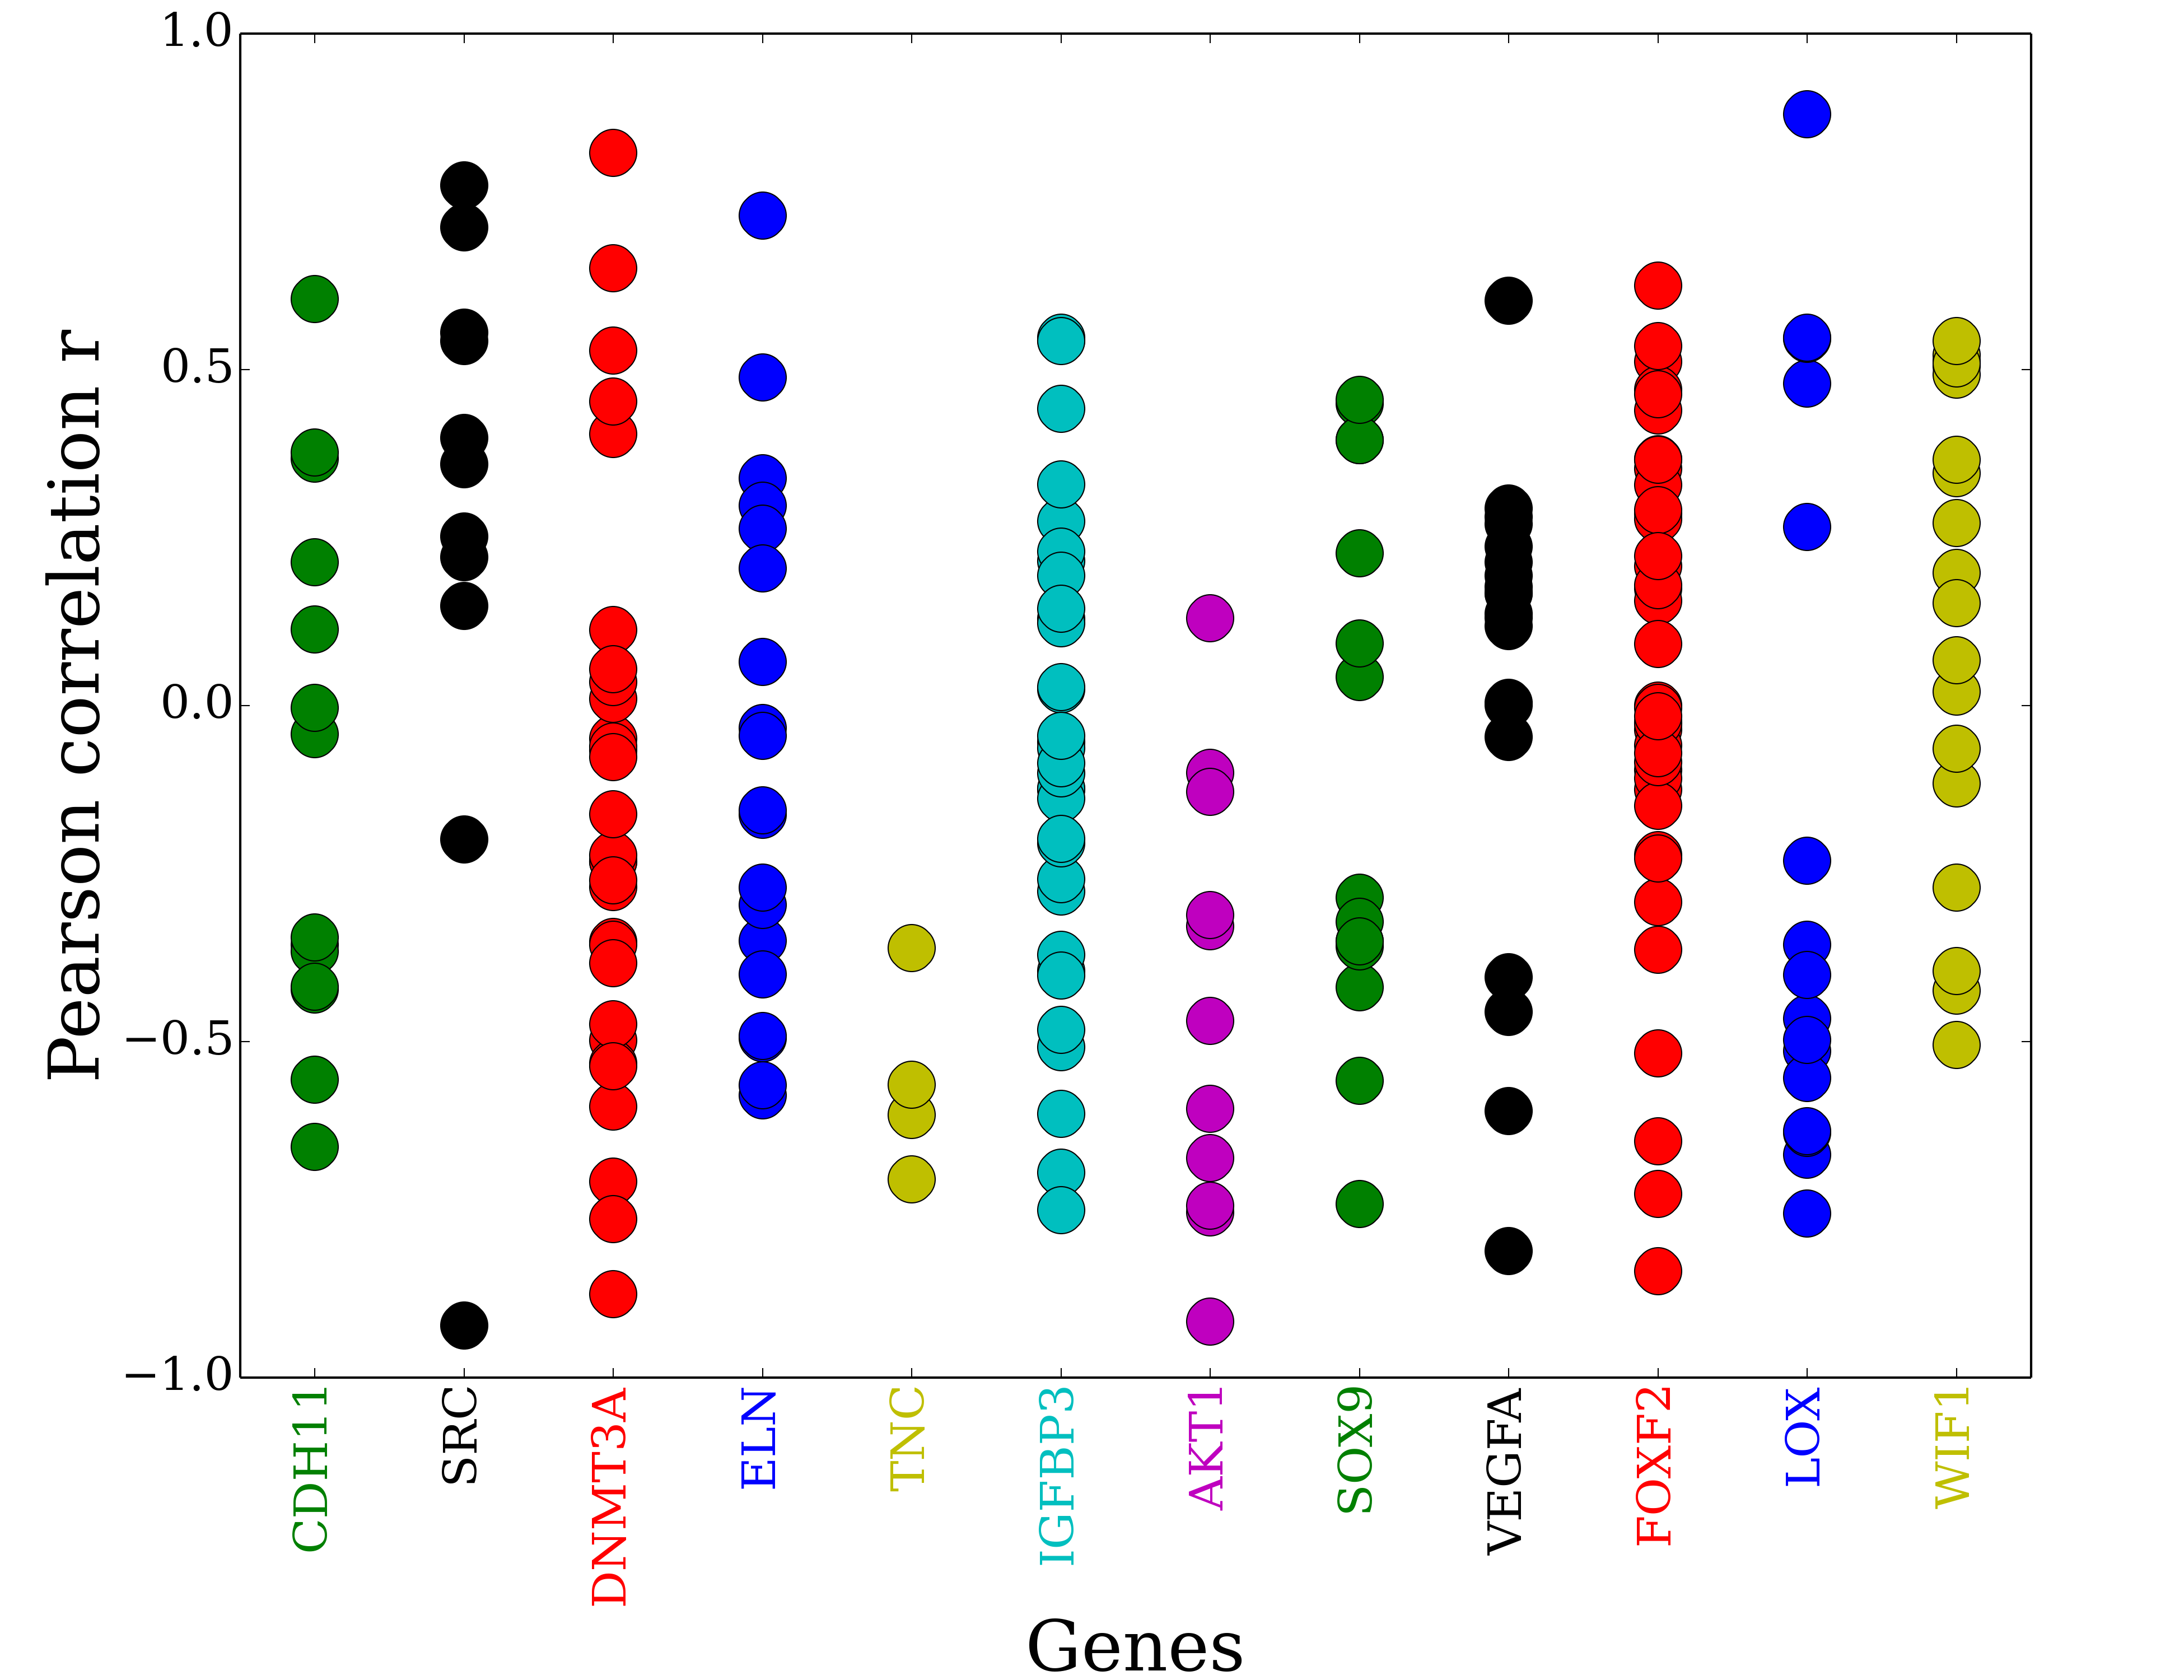
\includegraphics[scale=0.25]{{plots/meth/jointfigures_best/abs/valdist}.png}
\caption{Distribution of gene expression correlation for loci of each gene}
\label{fig:sup6}
\end{figure}
\clearpage

\section*{Supplementary Tables}

\begin{table}[ht]
\centering
\begin{tabular}{|c|c|c|c|c|}
\hline
Gene & Number of loci  & & Gene & Number of loci  \\
\hline
Cdh11 & 14 & & Zfp536 & 16 \\
\hline
Src & 11 & & Igfbp3 & 34 \\
\hline
Sox9 & 16 & & Wif1 & 21 \\
\hline
Dnmt3a & 41 & & Vegfa & 20 \\
\hline
Eln & 20 & & Tnc & 4 \\
\hline
Foxf2 & 41 & & Lox & 17 \\
\hline
Akt1 & 11 & & &  \\
\hline
\end{tabular}
\caption{Summary of methylation dataset}
\label{tab:sup1}
\end{table}
\clearpage

% \begin{table}
% \centering
% \begin{tabular}{|c|c|c|c|c|}
% \hline
% Gene & $r$  & & Gene & $r$ \\
% \hline
% Cdh11 & $0.60$ & & Lox & $0.88$ \\
% \hline
% Src & $0.77$ & & Igfbp3 & $0.55$ \\
% \hline
% Sox9 & $0.45$ & & Wif1 & $0.54$ \\
% \hline
% Dnmt3a & $0.82$ & & Vegfa & $0.60$ \\
% \hline
% Eln & $0.72$ & & Tnc & $-0.36$ \\
% \hline
% Foxf2 & $0.62$ & & & \\
% \hline
% Akt1 & $0.13$ & & &  \\
% \hline
% \end{tabular}
% \caption{Pearson correlation $r$  between expression and
%   methylation datasets over $8$ time points for each gene.}
% \label{tab:sup2}
% \end{table}

\begin{table}[ht]
\centering
\begin{tabular}{|c|c|c|c|c|}
\hline
Gene & $r$  & & Gene & $r$ \\
\hline
Cdh11 & $-0.65$ & & Lox & $0.88$ \\
\hline
Src & $-0.92$ & & Igfbp3 & $-0.75$ \\
\hline
Sox9 & $-0.74$ & & Wif1 & $0.54$ \\
\hline
Dnmt3a & $-0.876$ & & Vegfa & $-0.81$ \\
\hline
Eln & $0.72$ & & Tnc & $-0.70$ \\
\hline
Foxf2 & $-0.84$ & & & \\
\hline
Akt1 & $-0.91$ & & &  \\
\hline
\end{tabular}
\caption{Pearson correlation $r$  between expression and
  methylation datasets over $8$ time points for each gene.}
\label{tab:sup2}
\end{table}

\newpage

\bibliographystyle{plain}
\bibliography{expressbib}

\end{document}
